% $eader: /u/gcmpack/manual/part6/part6.tex,v 1.40 2006/06/27 22:34:09 edhill Exp $
% $Name:  $

\chapter{Physical Parameterizations - Packages I}
\label{chap:packagesI}

\begin{rawhtml}
<!-- CMIREDIR:packages: -->
\end{rawhtml}

In this chapter and in the following chapter, the MITgcm ``packages'' are 
described. While you can carry out many experiments with MITgcm by starting 
from case studies in section \ref{sect:tutorials}, configuring
a brand new experiment or making major changes to an experimental configuration
requires some knowledge of the {\it packages}
that make up the full MITgcm code. Packages are used in MITgcm to
help organize and layer various code building blocks that are assembled 
and selected to perform a specific experiment. Each of the specific experiments
described in section \ref{sect:tutorials} uses a particular combination
of packages.
Figure \ref{fig:package_organigramme} shows the full set of packages that
are available. As shown in the figure packages are classified into different 
groupings that layer on top of each other. The top layer packages are 
generally specialized to specific simulation types. In this layer there are
packages that deal with biogeochemical processes, ocean interior
and boundary layer processes, atmospheric processes, sea-ice, coupled 
simulations and state estimation.
Below this layer are a set of general purpose
numerical and computational packages. The general purpose numerical packages
provide code for kernel numerical alogorithms
that apply to
many different simulation types. Similarly, the general purpose computational 
packages implement non-numerical alogorithms that provide parallelism,
I/O and time-keeping functions that are used in many different scenarios.


\begin{figure}
%%\begin{minipage}{12cm}
%%\marginsize{0cm}{0cm}{0cm}{0cm}
%% \scalefig{0.6}
%% \epsfbox{part6/organigramme_mitgcm_pkg.eps}
%%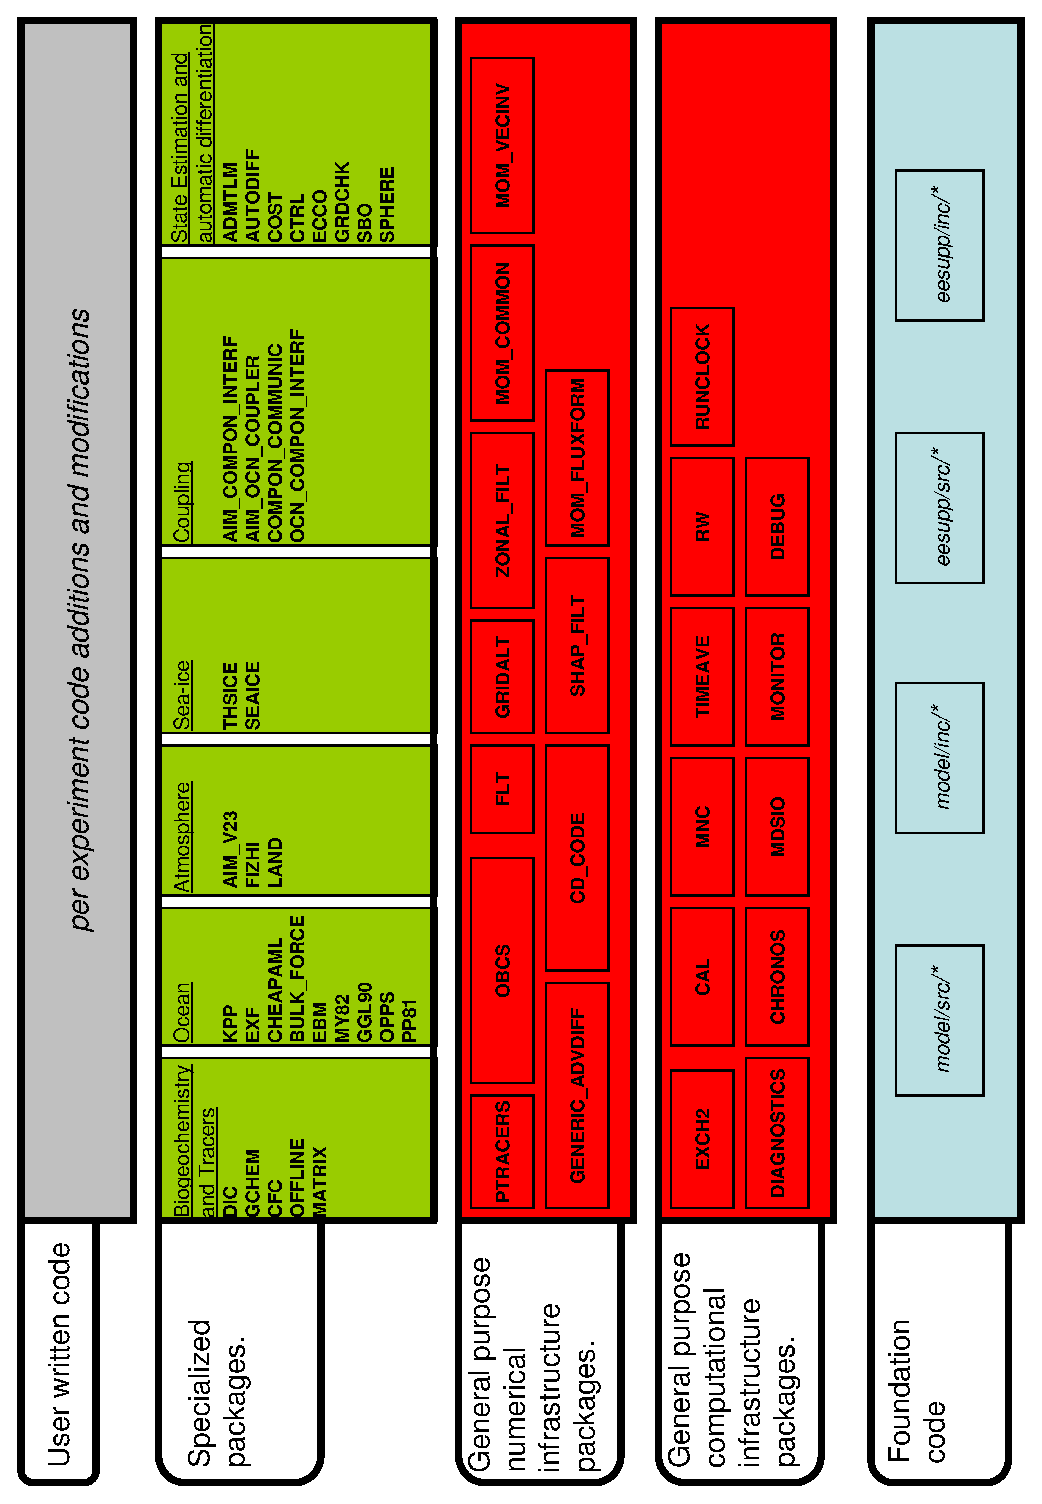
\epsfig{file=part6/organigramme_mitgcm_pkg.eps, angle=-90, scale=0.85, width=17cm}
%%\end{minipage}
\resizebox{5.5in}{!}{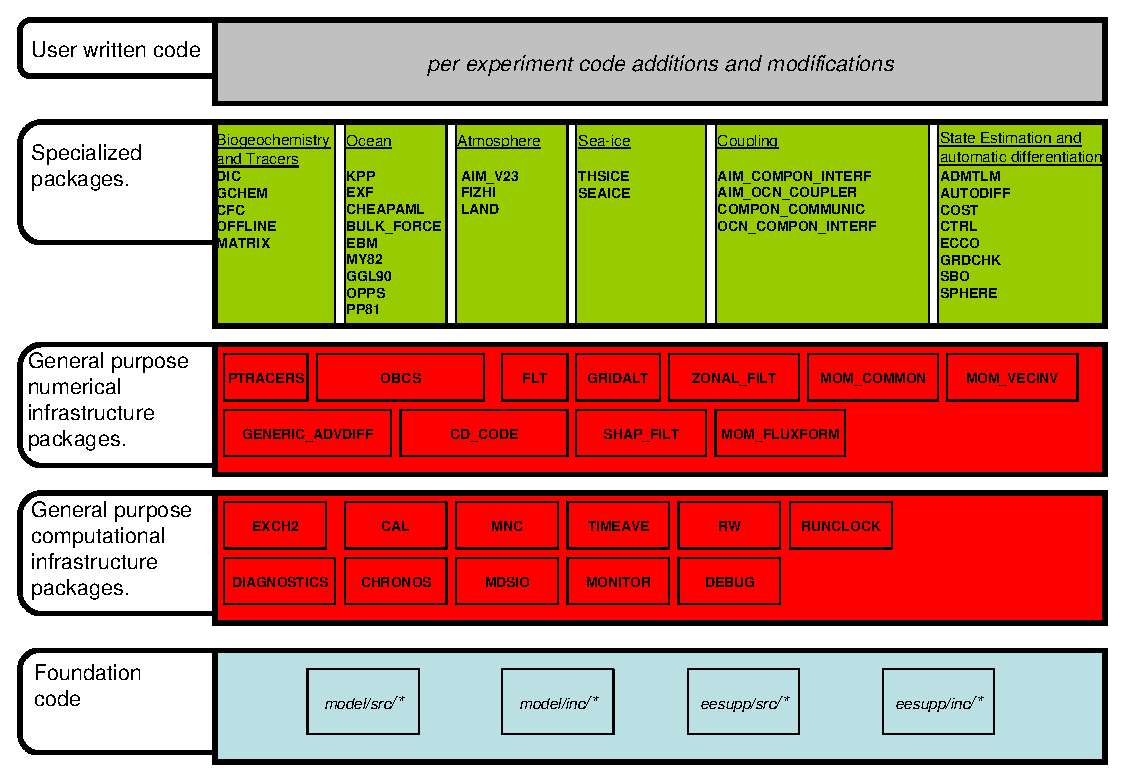
\includegraphics{part6/organigramme_mitgcm_pkg2.eps}}
\label{fig:package_organigramme}
\caption{ Hierarchy of code layers that are assembled to make up an MITgcm 
simulation. Conceptually (and in terms of code organization) MITgcm consists
of several layers. At the base is a layer of core software that provides a 
basic numerical and computational foundation for MITgcm simulations. This 
layer is shown marked {\bf Foundation Code} at the bottom of the figure
and corresponds to code in the italicised subdirectories on the figure.
This layer is not organized into packages. All code above the foundation layer
is organized as packages.  Much of the code in MITgcm is contained in packages 
which serve as a useful way of organizing and layering the different levels of 
functionality that make up the full MITgcm software distribution.
The figure shows the different packages in MITgcm as boxes containing bold 
face upper case names.  Directly above the foundation layer are two layers of 
general purpose infrastructure software that consist of computational and 
numerical packages.  These general purpose packages can be applied to both 
online and offline simulations and are used in many different physical 
simulation types.  Above these layers are more specialized packages.  }
\end{figure}

The following sections describe the packages shown in 
figure \ref{fig:package_organiigramme}. Section \ref{sec:pkg:using}
describes the general procedure for using any package in MITgcm.
Following that sections \ref{}-\ref{} 
layout the algorithms implemented in specific packages
and describe how to use the individual packages. A brief synopsis of the 
function of each package is given in table \ref{tab:package_summary_tab}.
Organizationally package code is assigned a
separate subdirectory in the MITgcm code distribution
(within the source code directory \texttt{pkg}).
The name of this subdirectory is used as the package name in
table \ref{tab:package_summary_tab}.

%% In this chapter the schemes for parameterizing processes that are not
%% represented explicitly in MITgcm are described.  Some of these
%% processes are sub-grid scale (SGS) phenomena, other processes, such as
%% open-boundaries, are external to the simulation.

% Overview
\newpage
% $Header: /u/gcmpack/manual/s_phys_pkgs/text/packages.tex,v 1.3 2004/02/12 16:40:28 edhill Exp $
% $Name:  $

\section{Using MITgcm Packages}

The set of packages that will be used within a partiucular model can
be configured using a combination of both ``compile--time'' and
``run--time'' options.  Compile--time options are those used to select
which packages will be ``compiled in'' or implemented within the
program.  Packages excluded at compile time are completely absent from
the executable program(s) and thus cannot be later activated by any
set of subsequent run--time options.

\subsection{Package Inclusion/Exclusion}

There are numerous ways that one can specify compile--time package
inclusion or exclusion and they are all implemented by the
\texttt{genmake2} program which was previously described in Section
\ref{sect:buildingCode}.  The options are as follows:
\begin{enumerate}
\item Setting the \texttt{genamake2} options \texttt{--enable PKG}
  and/or \texttt{--disable PKG} specifies inclusion or exclusion.
  This method is intended as a convenient way to perform a single
  (perhaps for a quick test) compilation.
  
\item By creating a text file with the name \texttt{packages.conf} in
  either the local build directory or the \texttt{-mods=DIR}
  directory, one can specify a list of packages (one package per line,
  with '\texttt{\#}' as the comment character) to be included.  Since
  the \texttt{packages.conf} file can be saved, this is the preferred
  method for setting and recording (for future reference) the package
  configuration.
  
\item For convenience, a list of ``standard'' package groups is
  contained in the \texttt{pkg/pkg\_groups} file.  By selecting one of
  the package group names in the \texttt{packages.conf} file, one
  automatically obtains all packages in that group.

\item By default (that is, if a \texttt{packages.conf} file is not
  found), the \texttt{genmake2} program will use the contents of the
  \texttt{pkg/pkg\_default} file to obtain a list of packages.

\item To help prevent users from creating unusable package groups, the
  \texttt{genmake2} program will parse the contents of the
  \texttt{pkg/pkg\_depend} file to determine:
  \begin{itemize}
  \item whether any two requested packages cannot be simultaneously
    included (\textit{eg.} \textit{seaice} and \textit{thsice} are
    mutually exclusive),
  \item whether additional packages must be included in order to
    satisfy package dependencies (\textit{eg.} \textit{rw} depends
    upon functionality within the \textit{mdsio} package), and
  \item whether the set of all requested packages is compatible with
    the dependencies (and producing an error if they aren't).
  \end{itemize}
  Thus, as a result of the dependencies, additional packages may be
  added to those originally requested.

\end{enumerate}


\subsection{Package Activation}

For run--time package control, MITgcm uses flags set through a
\texttt{data.pkg} file.  While some packages (\textit{eg.}
\texttt{debug}, \texttt{mnc}, \texttt{exch2}) may have their own usage
conventions, most follow a simple flag naming convention of the form:
\begin{verbatim}
  usePackageName=.TRUE.
\end{verbatim}
where the \texttt{usePackageName} variable can activate or disable the
package at runtime.  As mentioned previously, packages must be
included in order to be activated.  Generally, such mistakes will be
detected and reported as errors by the code.  However, users should
still be aware of the dependency.


\section{Package Coding Standards}

The following sections describe how to modify and/or create new MITgcm
packages.

\subsection{Packages are Not Libraries}

To a beginner, the MITgcm packages may resemble libraries as used in
myriad software projects.  While future versions are likely to
implement packages as libraries (perhaps using FORTRAN90/95 syntax)
the current packages (FORTRAN77) are \textbf{not} based upon any
concept of libraries.

\subsubsection{File Inclusion Rules}

Instead, packages should be viewed only as directories containing
``sets of source files'' that are built using some simple mechanisms
provided by \texttt{genmake2}.  Conceptually, the build process adds
files as they are found and proceeds according to the following rules:
\begin{enumerate}
\item \texttt{genmake2} locates a ``core'' or main set of source files
  (the \texttt{-standarddirs} option sets these locations and the
  default value contains the directories \texttt{eesupp} and
  \texttt{model}).
  
\item \texttt{genmake2} then finds additional source files by
  inspecting the contents of each of the package directories:
  \begin{enumerate}
  \item As the new files are found, they are added to a list of source
    files.

  \item If there is a file name ``collision'' (that is, if one of the
    files in a package has the same name as one of the files
    previously encountered) then the file within the newer (more
    recently visited) package will superseed (or ``hide'') any
    previous file(s) with the same name.
    
  \item Packages are visited (and thus files discovered) {\it in the
      order that the packages are enabled} within \texttt{genmake2}.
    Thus, the files in \texttt{PackB} may superseed the files in
    \texttt{PackA} if \texttt{PackA} is enabled before \texttt{PackB}.
    Thus, package ordering can be significant!  For this reason,
    \texttt{genmake2} honors the order in which packages are
    specified.
  \end{enumerate}
\end{enumerate}

These rules were adopted since they provide a relatively simple means
for rapidly including (or ``hiding'') existing files with modified
versions.

\subsubsection{Conditional Compilation and \texttt{PACKAGES\_CONFIG.h}}

Given that packages are simply groups of files that may be added or
removed to form a whole, one may wonder how linking (that is, FORTRAN
symbol resolution) is handled.  This is the second way that
\texttt{genmake2} supports the concept of packages.  Basically,
\texttt{genmake2} creates a \texttt{Makefile} that, in turn, is able
to create a file called \texttt{PACKAGES\_CONFIG.h} that contains a set
of C pre-processor (or ``CPP'') directives such as:
\begin{verbatim}
   #undef  ALLOW_KPP
   #undef  ALLOW_LAND
   ...
   #define ALLOW_GENERIC_ADVDIFF
   #define ALLOW_MDSIO
   ...
\end{verbatim}
These CPP symbols are then used throughout the code to conditionally
isolate variable definitions, function calls, or any other code that
depends upon the presence or absence of any particular package.

An example illustrating the use of these defines is:
\begin{verbatim}
   #ifdef ALLOW_GMREDI
         IF (useGMRedi) CALL GMREDI_CALC_DIFF(
        I        bi,bj,iMin,iMax,jMin,jMax,K,
        I        maskUp,
        O        KappaRT,KappaRS,
        I        myThid)
   #endif
\end{verbatim}
which is included from the file
\filelink{calc\_diffusivity.F}{model-src-calc_diffusivity.F}
and shows how both the compile--time \texttt{ALLOW\_GMREDI} flag and the
run--time \texttt{useGMRedi} are nested.

There are some benefits to using the technique described here.  The
first is that code snippets or subroutines associated with packages
can be placed or called from almost anywhere else within the code.
The second benefit is related to memory footprint and performance.
Since unused code can be removed, there is no performance penalty due
to unnecessary memory allocation, unused function calls, or extra
run-time \texttt{IF (...)} conditions.  The major problems with this
approach are the potentially difficult-to-read and difficult-to-debug
code caused by an overuse of CPP statements.  So while it can be done,
developers should exerecise some discipline and avoid unnecesarily
``smearing'' their package implementation details across numerous
files.


\subsubsection{Package Startup or Boot Sequence}

Calls to package routines within the core code timestepping loop can
vary.  However, all packages should follow a required "boot" sequence
outlined here:

{\footnotesize
\begin{verbatim}
    1. S/R PACKAGES_BOOT()
            :
        CALL OPEN_COPY_DATA_FILE( 'data.pkg', 'PACKAGES_BOOT', ... )
 

    2. S/R PACKAGES_READPARMS()
            :
        #ifdef ALLOW_${PKG}
          if ( use${Pkg} )
     &       CALL ${PKG}_READPARMS( retCode )
        #endif

    3. S/R PACKAGES_INIT_FIXED()
            :
        #ifdef ALLOW_${PKG}
          if ( use${Pkg} )
     &       CALL ${PKG}_INIT_FIXED( retCode )
        #endif

    4. S/R PACKAGES_CHECK()
            :
        #ifdef ALLOW_${PKG}
          if ( use${Pkg} )
     &       CALL ${PKG}_CHECK( retCode )
        #else
          if ( use${Pkg} )
     &       CALL PACKAGES_CHECK_ERROR('${PKG}')
        #endif

    5. S/R PACKAGES_INIT_VARIABLES()
            :
        #ifdef ALLOW_${PKG}
          if ( use${Pkg} )
     &       CALL ${PKG}_INIT_VARIA( )
        #endif

     6. S/R DO_THE_MODEL_IO

        #ifdef ALLOW_${PKG}
          if ( use${Pkg} )
     &       CALL ${PKG}_DIAGS( )
        #endif

     7. S/R PACKAGES_WRITE_PICKUP()

        #ifdef ALLOW_${PKG}
          if ( use${Pkg} )
     &       CALL ${PKG}_WRITE_PICKUP( )
        #endif\end{verbatim}
}


\subsubsection{Package Startup or Boot Sequence}



% Packages Related to Hydrodynamical Kernel
\newpage
\section{Packages Related to Hydrodynamical Kernel}
% $Header: /u/gcmpack/manual/s_phys_pkgs/text/generic_advdiff.tex,v 1.3 2004/10/12 18:16:03 edhill Exp $
% $Name:  $


\section{Generic Advection/Diffusion}
\label{sec:pkg:gad}
\begin{rawhtml}
<!-- CMIREDIR:package_gad: -->
\end{rawhtml}

The {\tt generic\_advdiff} package provides...


\subsection{Introduction}
Package {\tt generic\_advdiff} is a...


\subsection{Key subroutines, parameters and files}
\label{sec:pkg:rw:implementation_synopsis}
The {\tt generic\_advdiff} package has... 




\newpage
\subsection{FFT Filtering Code}
\label{sec:zonal_filt}
\begin{rawhtml}
<!-- CMIREDIR:package_zonal_filt: -->
\end{rawhtml}

\subsubsection{Key subroutines, parameters and files}
\label{sec:pkg:zonal_filt:implementation_synopsis}

\subsubsection{Experiments and tutorials that use zonal filter}
\label{sec:pkg:zonal_filt:experiments}

\begin{itemize}
\item{Held Suarez tutorial, in tutorial\_held\_suarez\_cs verification directory, described in 
section \ref{sect:eg-hs} }
\end{itemize}



\newpage
% $Header: /u/gcmpack/manual/s_phys_pkgs/text/exch2.tex,v 1.27 2009/05/02 02:13:18 jmc Exp $
% $Name:  $

%%  * Introduction
%%    o what it does, citations (refs go into mitgcm_manual.bib, 
%%      preferably in alphabetic order)
%%    o Equations 
%%  * Key subroutines and parameters
%%  * Reference material (auto generated from Protex and structured comments)
%%    o automatically inserted at \section{Reference} 


\subsection{exch2: Extended Cubed Sphere \mbox{Topology}}
\label{sec:exch2}


\subsubsection{Introduction}

The \texttt{exch2} package extends the original cubed sphere topology
configuration to allow more flexible domain decomposition and
parallelization.  Cube faces (also called subdomains) may be divided
into any number of tiles that divide evenly into the grid point
dimensions of the subdomain.  Furthermore, the tiles can run on
separate processors individually or in groups, which provides for
manual compile-time load balancing across a relatively arbitrary
number of processors.

The exchange parameters are declared in
\filelink{pkg/exch2/W2\_EXCH2\_TOPOLOGY.h}{pkg-exch2-W2_EXCH2_TOPOLOGY.h}
and assigned in
\filelink{pkg/exch2/w2\_e2setup.F}{pkg-exch2-w2_e2setup.F}. The
validity of the cube topology depends on the \file{SIZE.h} file as
detailed below.  The default files provided in the release configure a
cubed sphere topology of six tiles, one per subdomain, each with
32$\times$32 grid points, with all tiles running on a single processor.  Both
files are generated by Matlab scripts in
\file{utils/exch2/matlab-topology-generator}; see Section
\ref{sec:topogen} \sectiontitle{Generating Topology Files for exch2}
for details on creating alternate topologies.  Pregenerated examples
of these files with alternate topologies are provided under
\file{utils/exch2/code-mods} along with the appropriate \file{SIZE.h}
file for single-processor execution.

\subsubsection{Invoking exch2}

To use exch2 with the cubed sphere, the following conditions must be
met:

\begin{itemize}
\item The exch2 package is included when \file{genmake2} is run.  The
  easiest way to do this is to add the line \code{exch2} to the
  \file{packages.conf} file -- see Section \ref{sect:buildingCode}
  \sectiontitle{Building the code} for general
  details.

\item An example of \file{W2\_EXCH2\_TOPOLOGY.h} and
  \file{w2\_e2setup.F} must reside in a directory containing files
  symbolically linked by the \file{genmake2} script.  The safest place
  to put these is the directory indicated in the \code{-mods=DIR}
  command line modifier (typically \file{../code}), or the build
  directory.  The default versions of these files reside in
  \file{pkg/exch2} and are linked automatically if no other versions
  exist elsewhere in the build path, but they should be left untouched
  to avoid breaking configurations other than the one you intend to
  modify.

\item Files containing grid parameters, named \file{tile00$n$.mitgrid}
  where $n$=\code{(1:6)} (one per subdomain), must be in the working
  directory when the MITgcm executable is run.  These files are
  provided in the example experiments for cubed sphere configurations
  with 32$\times$32 cube sides -- please contact MITgcm support if you
  want to generate files for other configurations.

\item As always when compiling MITgcm, the file \file{SIZE.h} must be
  placed where \file{genmake2} will find it.  In particular for exch2,
  the domain decomposition specified in \file{SIZE.h} must correspond
  with the particular configuration's topology specified in
  \file{W2\_EXCH2\_TOPOLOGY.h} and \file{w2\_e2setup.F}.  Domain
  decomposition issues particular to exch2 are addressed in Section
  \ref{sec:topogen} \sectiontitle{Generating Topology Files for exch2}
  and \ref{sec:exch2mpi} \sectiontitle{exch2, SIZE.h, and
    Multiprocessing}; a more general background on the subject
  relevant to MITgcm is presented in Section
  \ref{sect:specifying_a_decomposition}
  \sectiontitle{Specifying a decomposition}.
\end{itemize}

At the time of this writing the following examples use exch2 and may
be used for guidance:

\begin{verbatim}
verification/adjust_nlfs.cs-32x32x1
verification/adjustment.cs-32x32x1 
verification/aim.5l_cs
verification/global_ocean.cs32x15
verification/hs94.cs-32x32x5
\end{verbatim}




\subsubsection{Generating Topology Files for exch2}
\label{sec:topogen}

Alternate cubed sphere topologies may be created using the Matlab
scripts in \file{utils/exch2/matlab-topology-generator}. Running the
m-file
\filelink{driver.m}{utils-exch2-matlab-topology-generator_driver.m}
from the Matlab prompt (there are no parameters to pass) generates
exch2 topology files \file{W2\_EXCH2\_TOPOLOGY.h} and
\file{w2\_e2setup.F} in the working directory and displays a figure of
the topology via Matlab -- figures \ref{fig:6tile}, \ref{fig:18tile}, 
and \ref{fig:48tile} are examples of the generated diagrams.  The other 
m-files in the directory are
subroutines called from \file{driver.m} and should not be run ``bare'' except
for development purposes. \\

The parameters that determine the dimensions and topology of the
generated configuration are \code{nr}, \code{nb}, \code{ng},
\code{tnx} and \code{tny}, and all are assigned early in the script. \\

The first three determine the height and width of the subdomains and
hence the size of the overall domain.  Each one determines the number
of grid points, and therefore the resolution, along the subdomain
sides in a ``great circle'' around each the three spatial axes of the cube.  At the time
of this writing MITgcm requires these three parameters to be equal,
but they provide for future releases  to accomodate different
resolutions around the axes to allow subdomains with differing resolutions.\\

The parameters \code{tnx} and \code{tny} determine the width and height of
the tiles into which the subdomains are decomposed, and must evenly
divide the integer assigned to \code{nr}, \code{nb} and \code{ng}.
The result is a rectangular tiling of the subdomain.  Figure
\ref{fig:48tile} shows one possible topology for a twenty-four-tile
cube, and figure \ref{fig:6tile} shows one for six tiles. \\

\begin{figure}
\begin{center}
 \resizebox{6in}{!}{
% \includegraphics{part6/s24t_16x16.ps}
  \includegraphics{part6/adjust_cs.ps}
 }
\end{center} 

\caption{Plot of a cubed sphere topology with a 32$\times$192 domain
divided into six 32$\times$32 subdomains, each of which is divided
into eight tiles of width \code{tnx=16} and height \code{tny=8} for a 
total of forty-eight tiles. The colored borders of the subdomains 
represent the parameters \code{nr} (red), \code{ng} (green), and
\code{nb} (blue). 
This tiling is used in the example
verification/adjustment.cs-32x32x1/
with the option (blanklist.txt) to remove the land-only 4 tiles 
(11,12,13,14) which are filled in red on the plot.
} \label{fig:48tile}
\end{figure}

\begin{figure}
\begin{center}
 \resizebox{6in}{!}{
% \includegraphics{part6/s12t_16x32.ps}
  \includegraphics{part6/polarcap.ps}
 }
\end{center} 
\caption{Plot of a non-square cubed sphere topology with 
6 subdomains of different size (nr=90,ng=360,nb=90),
divided into one to four tiles each
 (\code{tnx=90, tny=90}), resulting in a total of 18 tiles.
} \label{fig:18tile}
\end{figure}

\begin{figure}
\begin{center}
 \resizebox{4in}{!}{
% \includegraphics{part6/s6t_32x32.ps}
  \includegraphics{part6/s6t_32x32.ps}
 }
\end{center} 
\caption{Plot of a cubed sphere topology with a 32$\times$192 domain
divided into six 32$\times$32 subdomains with one tile each
(\code{tnx=32, tny=32}).  This is the default configuration.
  }
\label{fig:6tile}
\end{figure}


Tiles can be selected from the topology to be omitted from being
allocated memory and processors.  This tuning is useful in ocean
modeling for omitting tiles that fall entirely on land.  The tiles
omitted are specified in the file
\filelink{blanklist.txt}{utils-exch2-matlab-topology-generator_blanklist.txt}
by their tile number in the topology, separated by a newline. \\




\subsubsection{exch2, SIZE.h, and Multiprocessing}
\label{sec:exch2mpi}

Once the topology configuration files are created, the Fortran
\code{PARAMETER}s in \file{SIZE.h} must be configured to match.
Section \ref{sect:specifying_a_decomposition} \sectiontitle{Specifying
  a decomposition} provides a general description of domain
decomposition within MITgcm and its relation to \file{SIZE.h}. The
current section specifies constraints that the exch2 package imposes
and describes how to enable parallel execution with MPI.

As in the general case, the parameters \varlink{sNx}{sNx} and
\varlink{sNy}{sNy} define the size of the individual tiles, and so
must be assigned the same respective values as \code{tnx} and
\code{tny} in \file{driver.m}.

The halo width parameters \varlink{OLx}{OLx} and \varlink{OLy}{OLy}
have no special bearing on exch2 and may be assigned as in the general
case. The same holds for \varlink{Nr}{Nr}, the number of vertical
levels in the model.

The parameters \varlink{nSx}{nSx}, \varlink{nSy}{nSy},
\varlink{nPx}{nPx}, and \varlink{nPy}{nPy} relate to the number of
tiles and how they are distributed on processors.  When using exch2,
the tiles are stored in the $x$ dimension, and so
\code{\varlink{nSy}{nSy}=1} in all cases.  Since the tiles as
configured by exch2 cannot be split up accross processors without
regenerating the topology, \code{\varlink{nPy}{nPy}=1} as well.

The number of tiles MITgcm allocates and how they are distributed
between processors depends on \varlink{nPx}{nPx} and
\varlink{nSx}{nSx}.  \varlink{nSx}{nSx} is the number of tiles per
processor and \varlink{nPx}{nPx} is the number of processors.  The
total number of tiles in the topology minus those listed in
\file{blanklist.txt} must equal \code{nSx*nPx}.  Note that in order to
obtain maximum usage from a given number of processors in some cases,
this restriction might entail sharing a processor with a tile that
would otherwise be excluded because it is topographically outside of
the domain and therefore in \file{blanklist.txt}.  For example,
suppose you have five processors and a domain decomposition of
thirty-six tiles that allows you to exclude seven tiles.  To evenly
distribute the remaining twenty-nine tiles among five processors, you
would have to run one ``dummy'' tile to make an even six tiles per
processor.  Such dummy tiles are \emph{not} listed in
\file{blanklist.txt}.

The following is an example of \file{SIZE.h} for the six-tile
configuration illustrated in figure \ref{fig:6tile} 
running on one processor:

\begin{verbatim}
      PARAMETER (
     &           sNx =  32,
     &           sNy =  32,
     &           OLx =   2,
     &           OLy =   2,
     &           nSx =   6,
     &           nSy =   1,
     &           nPx =   1,
     &           nPy =   1,
     &           Nx  = sNx*nSx*nPx,
     &           Ny  = sNy*nSy*nPy,
     &           Nr  =   5)
\end{verbatim}

The following is an example for the forty-eight-tile topology in
figure \ref{fig:48tile} running on six processors:

\begin{verbatim}
      PARAMETER (
     &           sNx =  16,
     &           sNy =   8,
     &           OLx =   2,
     &           OLy =   2,
     &           nSx =   8,
     &           nSy =   1,
     &           nPx =   6,
     &           nPy =   1,
     &           Nx  = sNx*nSx*nPx,
     &           Ny  = sNy*nSy*nPy,
     &           Nr  =   5)
\end{verbatim}


\subsubsection{Key Variables}

The descriptions of the variables are divided up into scalars,
one-dimensional arrays indexed to the tile number, and two and
three-dimensional arrays indexed to tile number and neighboring tile.
This division reflects the functionality of these variables: The
scalars are common to every part of the topology, the tile-indexed
arrays to individual tiles, and the arrays indexed by tile and
neighbor to relationships between tiles and their neighbors. \\

Scalars:

The number of tiles in a particular topology is set with the parameter
\code{NTILES}, and the maximum number of neighbors of any tiles by
\code{MAX\_NEIGHBOURS}.  These parameters are used for defining the
size of the various one and two dimensional arrays that store tile
parameters indexed to the tile number and are assigned in the files
generated by \file{driver.m}.\\

The scalar parameters \varlink{exch2\_domain\_nxt}{exch2_domain_nxt}
and \varlink{exch2\_domain\_nyt}{exch2_domain_nyt} express the number
of tiles in the $x$ and $y$ global indices.  For example, the default
setup of six tiles (Fig. \ref{fig:6tile}) has
\code{exch2\_domain\_nxt=6} and \code{exch2\_domain\_nyt=1}.  A
topology of forty-eight tiles, eight per subdomain (as in figure
\ref{fig:48tile}), will have \code{exch2\_domain\_nxt=12} and
\code{exch2\_domain\_nyt=4}.  Note that these parameters express the
tile layout in order to allow global data files that are tile-layout-neutral.
They have no bearing on the internal storage of the arrays.  The tiles
are stored internally in a range from \code{\varlink{bi}{bi}=(1:NTILES)} in the
$x$ axis, and the $y$ axis variable \varlink{bj}{bj} is assumed to 
equal \code{1} throughout the package. \\

Arrays indexed to tile number:

The following arrays are of length \code{NTILES} and are indexed to
the tile number, which is indicated in the diagrams with the notation
\textsf{t}$n$.  The indices are omitted in the descriptions. \\

The arrays \varlink{exch2\_tnx}{exch2_tnx} and
\varlink{exch2\_tny}{exch2_tny} express the $x$ and $y$ dimensions of
each tile.  At present for each tile \texttt{exch2\_tnx=sNx} and
\texttt{exch2\_tny=sNy}, as assigned in \file{SIZE.h} and described in
Section \ref{sec:exch2mpi} \sectiontitle{exch2, SIZE.h, and
Multiprocessing}.  Future releases of MITgcm may allow varying tile
sizes. \\

The arrays \varlink{exch2\_tbasex}{exch2_tbasex} and
\varlink{exch2\_tbasey}{exch2_tbasey} determine the tiles' 
Cartesian origin within a subdomain  
and locate the edges of different tiles relative to each other.  As
an example, in the default six-tile topology (Fig. \ref{fig:6tile})
each index in these arrays is set to \code{0} since a tile occupies
its entire subdomain.  The twenty-four-tile case discussed above will
have values of \code{0} or \code{16}, depending on the quadrant of the
tile within the subdomain.  The elements of the arrays
\varlink{exch2\_txglobalo}{exch2_txglobalo} and
\varlink{exch2\_txglobalo}{exch2_txglobalo} are similar to
\varlink{exch2\_tbasex}{exch2_tbasex} and
\varlink{exch2\_tbasey}{exch2_tbasey}, but locate the tile edges within the
global address space, similar to that used by global output and input
files. \\

The array \varlink{exch2\_myFace}{exch2_myFace} contains the number of
the subdomain of each tile, in a range \code{(1:6)} in the case of the
standard cube topology and indicated by \textbf{\textsf{f}}$n$ in
figures \ref{fig:6tile} and
\ref{fig:48tile}. \varlink{exch2\_nNeighbours}{exch2_nNeighbours}
contains a count of the neighboring tiles each tile has, and sets 
the bounds for looping over neighboring tiles.
\varlink{exch2\_tProc}{exch2_tProc} holds the process rank of each
tile, and is used in interprocess communication.  \\


The arrays \varlink{exch2\_isWedge}{exch2_isWedge},
\varlink{exch2\_isEedge}{exch2_isEedge},
\varlink{exch2\_isSedge}{exch2_isSedge}, and
\varlink{exch2\_isNedge}{exch2_isNedge} are set to \code{1} if the
indexed tile lies on the edge of its subdomain, \code{0} if
not.  The values are used within the topology generator to determine
the orientation of neighboring tiles, and to indicate whether a tile
lies on the corner of a subdomain.  The latter case requires special
exchange and numerical handling for the singularities at the eight
corners of the cube. \\


Arrays Indexed to Tile Number and Neighbor:

The following arrays have vectors of length \code{MAX\_NEIGHBOURS} and
\code{NTILES} and describe the orientations between the the tiles. \\

The array \code{exch2\_neighbourId(a,T)} holds the tile number
\code{Tn} for each of the tile number \code{T}'s neighboring tiles
\code{a}.  The neighbor tiles are indexed
\code{(1:exch2\_nNeighbours(T))} in the order right to left on the
north then south edges, and then top to bottom on the east then west
edges.  \\

 The \code{exch2\_opposingSend\_record(a,T)} array holds the
index \code{b} of the element in \texttt{exch2\_neighbourId(b,Tn)}
that holds the tile number \code{T}, given
\code{Tn=exch2\_neighborId(a,T)}.  In other words,
\begin{verbatim}
   exch2_neighbourId( exch2_opposingSend_record(a,T),
                      exch2_neighbourId(a,T) ) = T
\end{verbatim}
This provides a back-reference from the neighbor tiles. \\

The arrays \varlink{exch2\_pi}{exch2_pi} and
\varlink{exch2\_pj}{exch2_pj} specify the transformations of indices
in exchanges between the neighboring tiles.  These transformations are
necessary in exchanges between subdomains because a horizontal dimension 
in one subdomain 
may map to other horizonal dimension in an adjacent subdomain, and
may also have its indexing reversed. This swapping arises from the
``folding'' of two-dimensional arrays into a three-dimensional
cube. \\

The dimensions of \code{exch2\_pi(t,N,T)} and \code{exch2\_pj(t,N,T)}
are the neighbor ID \code{N} and the tile number \code{T} as explained
above, plus a vector of length \code{2} containing transformation
factors \code{t}.  The first element of the transformation vector
holds the factor to multiply the index in the same dimension, and the
second element holds the the same for the orthogonal dimension.  To
clarify, \code{exch2\_pi(1,N,T)} holds the mapping of the $x$ axis
index of tile \code{T} to the $x$ axis of tile \code{T}'s neighbor
\code{N}, and \code{exch2\_pi(2,N,T)} holds the mapping of \code{T}'s
$x$ index to the neighbor \code{N}'s $y$ index. \\
 
One of the two elements of \code{exch2\_pi} or \code{exch2\_pj} for a
given tile \code{T} and neighbor \code{N} will be \code{0}, reflecting
the fact that the two axes are orthogonal.  The other element will be
\code{1} or \code{-1}, depending on whether the axes are indexed in
the same or opposite directions.  For example, the transform vector of
the arrays for all tile neighbors on the same subdomain will be
\code{(1,0)}, since all tiles on the same subdomain are oriented
identically.  An axis that corresponds to the orthogonal dimension
with the same index direction in a particular tile-neighbor
orientation will have \code{(0,1)}.  Those with the opposite index
direction will have \code{(0,-1)} in order to reverse the ordering. \\

The arrays \varlink{exch2\_oi}{exch2_oi},
\varlink{exch2\_oj}{exch2_oj}, \varlink{exch2\_oi\_f}{exch2_oi_f}, and
\varlink{exch2\_oj\_f}{exch2_oj_f} are indexed to tile number and
neighbor and specify the relative offset within the subdomain of the
array index of a variable going from a neighboring tile \code{N} to a
local tile \code{T}.  Consider \code{T=1} in the six-tile topology
(Fig. \ref{fig:6tile}), where

\begin{verbatim}
       exch2_oi(1,1)=33
       exch2_oi(2,1)=0
       exch2_oi(3,1)=32
       exch2_oi(4,1)=-32
\end{verbatim}

The simplest case is \code{exch2\_oi(2,1)}, the southern neighbor,
which is \code{Tn=6}.  The axes of \code{T} and \code{Tn} have the
same orientation and their $x$ axes have the same origin, and so an
exchange between the two requires no changes to the $x$ index.  For
the western neighbor (\code{Tn=5}), \code{code\_oi(3,1)=32} since the
\code{x=0} vector on \code{T} corresponds to the \code{y=32} vector on
\code{Tn}.  The eastern edge of \code{T} shows the reverse case
(\code{exch2\_oi(4,1)=-32)}), where \code{x=32} on \code{T} exchanges
with \code{x=0} on \code{Tn=2}. \\

 The most interesting case, where \code{exch2\_oi(1,1)=33} and
\code{Tn=3}, involves a reversal of indices.  As in every case, the
offset \code{exch2\_oi} is added to the original $x$ index of \code{T}
multiplied by the transformation factor \code{exch2\_pi(t,N,T)}.  Here
\code{exch2\_pi(1,1,1)=0} since the $x$ axis of \code{T} is orthogonal
to the $x$ axis of \code{Tn}.  \code{exch2\_pi(2,1,1)=-1} since the
$x$ axis of \code{T} corresponds to the $y$ axis of \code{Tn}, but the
index is reversed.  The result is that the index of the northern edge
of \code{T}, which runs \code{(1:32)}, is transformed to
\code{(-1:-32)}. \code{exch2\_oi(1,1)} is then added to this range to
get back \code{(32:1)} -- the index of the $y$ axis of \code{Tn}
relative to \code{T}.  This transformation may seem overly convoluted
for the six-tile case, but it is necessary to provide a general
solution for various topologies. \\



Finally, \varlink{exch2\_itlo\_c}{exch2_itlo_c},
\varlink{exch2\_ithi\_c}{exch2_ithi_c},
\varlink{exch2\_jtlo\_c}{exch2_jtlo_c} and
\varlink{exch2\_jthi\_c}{exch2_jthi_c} hold the location and index
bounds of the edge segment of the neighbor tile \code{N}'s subdomain
that gets exchanged with the local tile \code{T}.  To take the example
of tile \code{T=2} in the forty-eight-tile topology
(Fig. \ref{fig:48tile}): \\

\begin{verbatim}
       exch2_itlo_c(4,2)=17
       exch2_ithi_c(4,2)=17
       exch2_jtlo_c(4,2)=0
       exch2_jthi_c(4,2)=33
\end{verbatim}
 
Here \code{N=4}, indicating the western neighbor, which is
\code{Tn=1}.  \code{Tn} resides on the same subdomain as \code{T}, so
the tiles have the same orientation and the same $x$ and $y$ axes.
The $x$ axis is orthogonal to the western edge and the tile is 16
points wide, so \code{exch2\_itlo\_c} and \code{exch2\_ithi\_c}
indicate the column beyond \code{Tn}'s eastern edge, in that tile's
halo region. Since the border of the tiles extends through the entire
height of the subdomain, the $y$ axis bounds \code{exch2\_jtlo\_c} to
\code{exch2\_jthi\_c} cover the height of \code{(1:32)}, plus 1 in
either direction to cover part of the halo. \\

For the north edge of the same tile \code{T=2} where \code{N=1} and 
the neighbor tile is \code{Tn=5}:

\begin{verbatim}
       exch2_itlo_c(1,2)=0
       exch2_ithi_c(1,2)=0
       exch2_jtlo_c(1,2)=0
       exch2_jthi_c(1,2)=17
\end{verbatim}
 
\code{T}'s northern edge is parallel to the $x$ axis, but since
\code{Tn}'s $y$ axis corresponds to \code{T}'s $x$ axis, \code{T}'s
northern edge exchanges with \code{Tn}'s western edge.  The western
edge of the tiles corresponds to the lower bound of the $x$ axis, so
\code{exch2\_itlo\_c} and \code{exch2\_ithi\_c} are \code{0}, in the 
western halo region of \code{Tn}. The range of
\code{exch2\_jtlo\_c} and \code{exch2\_jthi\_c} correspond to the
width of \code{T}'s northern edge, expanded by one into the halo. \\


\subsubsection{Key Routines}

Most of the subroutines particular to exch2 handle the exchanges
themselves and are of the same format as those described in
\ref{sect:cube_sphere_communication} \sectiontitle{Cube sphere
communication}.  Like the original routines, they are written as
templates which the local Makefile converts from \code{RX} into 
\code{RL} and \code{RS} forms. \\

The interfaces with the core model subroutines are
\code{EXCH\_UV\_XY\_RX}, \code{EXCH\_UV\_XYZ\_RX} and
\code{EXCH\_XY\_RX}.  They override the standard exchange routines
when \code{genmake2} is run with \code{exch2} option.  They in turn
call the local exch2 subroutines \code{EXCH2\_UV\_XY\_RX} and
\code{EXCH2\_UV\_XYZ\_RX} for two and three-dimensional vector
quantities, and \code{EXCH2\_XY\_RX} and \code{EXCH2\_XYZ\_RX} for two
and three-dimensional scalar quantities.  These subroutines set the
dimensions of the area to be exchanged, call \code{EXCH2\_RX1\_CUBE}
for scalars and \code{EXCH2\_RX2\_CUBE} for vectors, and then handle
the singularities at the cube corners. \\

The separate scalar and vector forms of \code{EXCH2\_RX1\_CUBE} and
\code{EXCH2\_RX2\_CUBE} reflect that the vector-handling subroutine
needs to pass both the $u$ and $v$ components of the physical vectors.
This swapping arises from the topological folding discussed above, where the
$x$ and $y$ axes get swapped in some cases, and is not an
issue with the scalar case. These subroutines call
\code{EXCH2\_SEND\_RX1} and \code{EXCH2\_SEND\_RX2}, which do most of
the work using the variables discussed above. \\

\subsubsection{Experiments and tutorials that use exch2}
\label{sec:pkg:exch2:experiments}

\begin{itemize}
\item{Held Suarez tutorial, in tutorial\_held\_suarez\_cs verification directory, 
described in section \ref{sect:eg-hs} }
\end{itemize}


\newpage
\subsection{Gridalt - Alternate Grid Package}
\label{sec:pkg:gridalt}
\begin{rawhtml}
<!-- CMIREDIR:package_gridalt: -->
\end{rawhtml}

\subsubsection {Introduction} 

The gridalt package is designed to allow different components of MITgcm to
be run using horizontal and/or vertical grids which are different from the main 
model grid. The gridalt routines handle the definition of the all the various
alternative grid(s) and the mappings between them and the MITgcm grid.
The implementation of the gridalt package which allows the high end atmospheric 
physics (fizhi) to be run on a high resolution and quasi terrain-following vertical 
grid is documented here.  The package has also (with some user modifications) been used 
for other calculations within the GCM. 

The rationale for implementing the atmospheric physics on a high resolution vertical
grid involves the fact that the MITgcm $p^*$ (or any pressure-type) coordinate cannot 
maintain the vertical resolution near the surface as the bottom topography rises above
sea level. The vertical length scales near the ground are small and can vary 
on small time scales, and the vertical grid must be adequate to resolve them.
Many studies with both regional and global atmospheric models have demonstrated the 
improvements in the simulations when the vertical resolution near the surface is 
increased (\cite{bm:99,Inn:01,wo:98,breth:99}). Some of the benefit of increased resolution 
near the surface is realized by employing the higher resolution for the computation of the 
forcing due to turbulent and convective processes in the atmosphere.  

The parameterizations of atmospheric subgrid scale processes are all essentially
one-dimensional in nature, and the computation of the terms in the equations of
motion due to these processes can be performed for the air column over one grid point 
at a time.  The vertical grid on which these computations take place can therefore be 
entirely independant of the grid on which the equations of motion are integrated, and 
the 'tendency' terms can be interpolated to the vertical grid on which the equations
of motion are integrated. A modified $p^*$ coordinate, which adjusts to the local 
terrain and adds additional levels between the lower levels of the existing $p^*$ grid 
(and perhaps between the levels near the tropopause as well), is implemented. The 
vertical discretization is different for each grid point, although it consist of the 
same number of levels. Additional 'sponge' levels aloft are added when needed. The levels 
of the physics grid are constrained to fit exactly into the existing $p^*$ grid, simplifying 
the mapping between the two vertical coordinates.  This is illustrated as follows:

\begin{figure}[htbp]
\vspace*{-0.4in}
\begin{center}
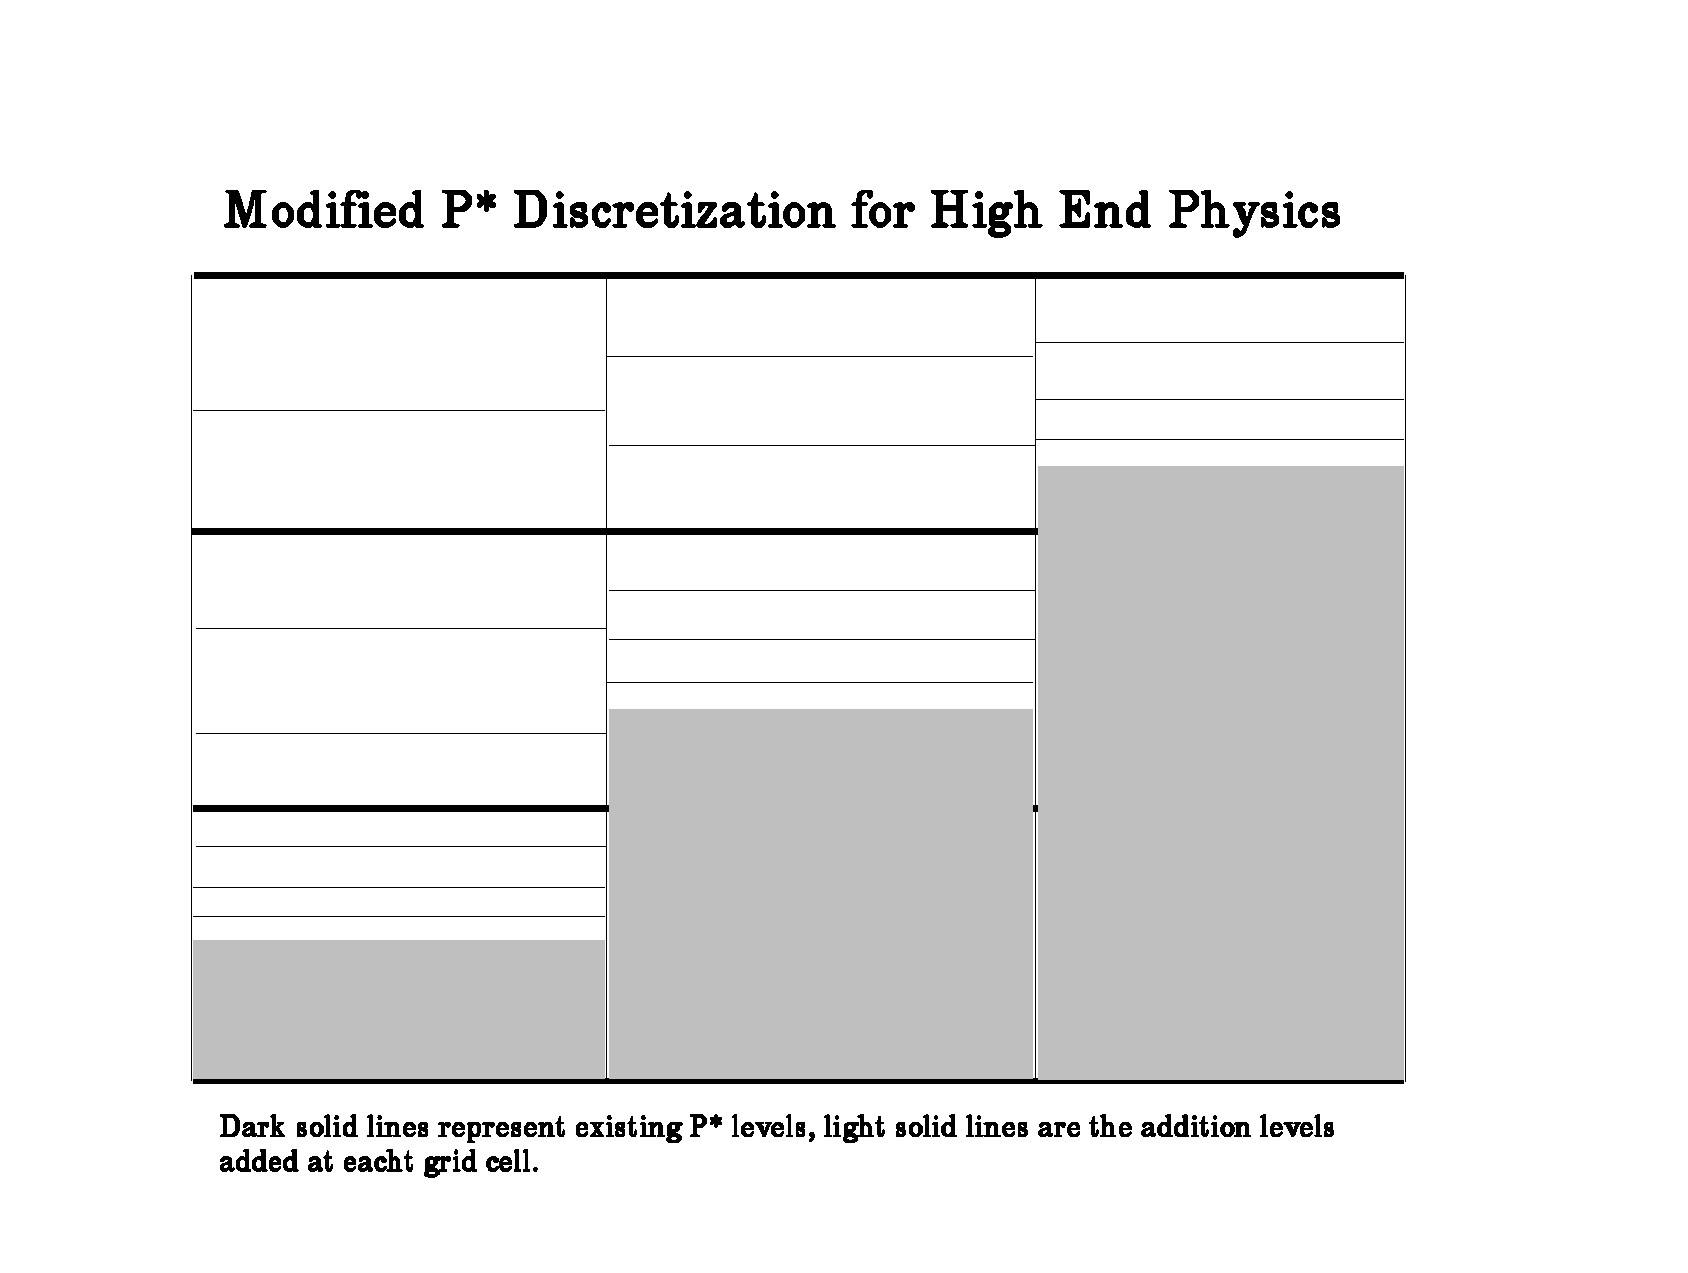
\includegraphics[height=2.4in]{part6/vertical.eps}
\caption{Vertical discretization for MITgcm (dark grey lines) and for the
atmospheric physics (light grey lines). In this implementation, all MITgcm level
interfaces must coincide with atmospheric physics level interfaces.}
\end{center}
\end{figure}

The algorithm presented here retains the state variables on the high resolution 'physics'
grid as well as on the coarser resolution 'dynamics` grid, and ensures that the two 
estimates of the state 'agree' on the coarse resolution grid.  It would have been possible 
to implement a technique in which the tendencies due to atmospheric physics are computed 
on the high resolution grid and the state variables are retained at low resolution only. 
This, however, for the case of the turbulence parameterization,  would mean that the 
turbulent kinetic energy source terms, and all the turbulence terms that are written 
in terms of gradients of the mean flow, cannot really be computed making use of the fine 
structure in the vertical. 

\subsubsection{Equations on Both Grids}

In addition to computing the physical forcing terms of the momentum, thermodynamic and humidity 
equations on the modified (higher resolution) grid, the higher resolution structure of the 
atmosphere (the boundary layer) is retained between physics calculations. This neccessitates
a second set of evolution equations for the atmospheric state variables on the modified grid. 
If the equation for the evolution of $U$ on $p^*$ can be expressed as:
\[
\left . {\partial U \over {\partial t}} \right |_{p^*}^{total} = 
\left . {\partial U \over {\partial t}} \right |_{p^*}^{dynamics} + 
\left . {\partial U \over {\partial t}} \right |_{p^*}^{physics}
\]
where the physics forcing terms on $p^*$ have been mapped from the modified grid, then an additional 
equation to govern the evolution of $U$ (for example) on the modified grid is written:
\[
\left . {\partial U \over {\partial t}} \right |_{p^{*m}}^{total} = 
\left . {\partial U \over {\partial t}} \right |_{p^{*m}}^{dynamics} + 
\left . {\partial U \over {\partial t}} \right |_{p^{*m}}^{physics} +
\gamma ({\left . U \right |_{p^*}} - {\left . U \right |_{p^{*m}}})
\]
where $p^{*m}$ refers to the modified higher resolution grid, and the dynamics forcing terms have 
been mapped from $p^*$ space.  The last term on the RHS is a relaxation term, meant to constrain
the state variables on the modified vertical grid to `track' the state variables on the $p^*$ grid 
on some time scale, governed by $\gamma$. In the present implementation, $\gamma = 1$, requiring
an immediate agreement between the two 'states'.

\subsubsection{Time stepping Sequence}
If we write $T_{phys}$ as the temperature (or any other state variable) on the high
resolution physics grid, and $T_{dyn}$ as the temperature on the coarse vertical resolution
dynamics grid, then:

\begin{enumerate}
%\itemsep{-0.05in}

\item{Compute the tendency due to physics processes.}

\item{Advance the physics state: ${{T^{n+1}}^{**}}_{phys}(l) = {T^n}_{phys}(l) + \delta T_{phys}$.}

\item{Interpolate the physics tendency to the dynamics grid, and advance the dynamics
state by physics and dynamics tendencies:
${T^{n+1}}_{dyn}(L) = {T^n}_{dyn}(L) + \delta T_{dyn}(L) + [\delta T _{phys}(l)](L)$.}

\item{Interpolate the dynamics tendency to the physics grid, and update the physics
grid due to dynamics tendencies: 
${{T^{n+1}}^*}_{phys}(l)$ = ${{T^{n+1}}^{**}}_{phys}(l) + {\delta T_{dyn}(L)}(l)$.}

\item{Apply correction term to physics state to account for divergence from dynamics state:
${T^{n+1}}_{phys}(l)$ = ${{T^{n+1}}^*}_{phys}(l) + \gamma \{  T_{dyn}(L) - [T_{phys}(l)](L) \}(l)$.} \\
Where $\gamma=1$ here. 

\end{enumerate}

\subsubsection{Interpolation}
In order to minimize the correction terms for the state variables on the alternative,
higher resolution grid, the vertical interpolation scheme must be constructed so that
a dynamics-to-physics interpolation can be exactly reversed with a physics-to-dynamics mapping.
The simple scheme employed to achieve this is:\\

Coarse to fine:\
For all physics layers l in dynamics layer L, $ T_{phys}(l) = \{T_{dyn}(L)\} = T_{dyn}(L) $.

Fine to coarse:\
For all physics layers l in dynamics layer L, $T_{dyn}(L) = [T_{phys}(l)] = \int{T_{phys} dp } $.\\

Where $\{\}$ is defined as the dynamics-to-physics operator and $[ ]$ is the physics-to-dynamics operator, $T$ stands for any state variable, and the subscripts $phys$ and $dyn$ stand for variables on
the physics and dynamics grids, respectively.

\subsubsection {Key subroutines, parameters and files } 

\noindent
One of the central elements of the gridalt package is the routine which 
is called from subroutine gridalt\_initialise to define the grid to be
used for the high end physics calculations. Routine make\_phys\_grid
passes back the parameters which define the grid, ultimately stored 
in the common block gridalt\_mapping.

\begin{verbatim}
       subroutine make_phys_grid(drF,hfacC,im1,im2,jm1,jm2,Nr,
     . Nsx,Nsy,i1,i2,j1,j2,bi,bj,Nrphys,Lbot,dpphys,numlevphys,nlperdyn)
c***********************************************************************
c Purpose: Define the grid that the will be used to run the high-end
c          atmospheric physics.
c
c Algorithm: Fit additional levels of some (~) known thickness in
c          between existing levels of the grid used for the dynamics
c
c Need:    Information about the dynamics grid vertical spacing
c
c Input:   drF         - delta r (p*) edge-to-edge
c          hfacC       - fraction of grid box above topography
c          im1, im2    - beginning and ending i - dimensions
c          jm1, jm2    - beginning and ending j - dimensions
c          Nr          - number of levels in dynamics grid
c          Nsx,Nsy     - number of processes in x and y direction
c          i1, i2      - beginning and ending i - index to fill
c          j1, j2      - beginning and ending j - index to fill
c          bi, bj      - x-dir and y-dir index of process
c          Nrphys      - number of levels in physics grid
c
c Output:  dpphys      - delta r (p*) edge-to-edge of physics grid
c          numlevphys  - number of levels used in the physics
c          nlperdyn    - physics level number atop each dynamics layer
c
c NOTES: 1) Pressure levs are built up from bottom, using p0, ps and dp:
c              p(i,j,k)=p(i,j,k-1) + dp(k)*ps(i,j)/p0(i,j)
c        2) Output dp's are aligned to fit EXACTLY between existing
c           levels of the dynamics vertical grid
c        3) IMPORTANT! This routine assumes the levels are numbered
c           from the bottom up, ie, level 1 is the surface.
c           IT WILL NOT WORK OTHERWISE!!!
c        4) This routine does NOT work for surface pressures less
c           (ie, above in the atmosphere) than about 350 mb
c***********************************************************************
\end{verbatim}

\noindent In the case of the grid used to compute the atmospheric physical
forcing (fizhi package), the locations of the grid points move in time with 
the MITgcm $p^*$ coordinate, and subroutine gridalt\_update is called during 
the run to update the locations of the grid points:

\begin{verbatim}
       subroutine gridalt_update(myThid)
c***********************************************************************
c Purpose: Update the pressure thicknesses of the layers of the
c          alternative vertical grid (used now for atmospheric physics).
c
c Calculate: dpphys    - new delta r (p*) edge-to-edge of physics grid
c                        using dpphys0 (initial value) and rstarfacC
c***********************************************************************
\end{verbatim}

\noindent The gridalt package also supplies utility routines which perform
the mappings from one grid to the other. These routines are called from the 
code which computes the fields on the alternative (fizhi) grid.

\begin{verbatim}
      subroutine dyn2phys(qdyn,pedyn,im1,im2,jm1,jm2,lmdyn,Nsx,Nsy,
     . idim1,idim2,jdim1,jdim2,bi,bj,windphy,pephy,Lbot,lmphy,nlperdyn,
     . flg,qphy)
C***********************************************************************
C Purpose:
C   To interpolate an arbitrary quantity from the 'dynamics' eta (pstar)
C               grid to the higher resolution physics grid
C Algorithm:
C   Routine works one layer (edge to edge pressure) at a time.
C   Dynamics -> Physics retains the dynamics layer mean value,
C   weights the field either with the profile of the physics grid
C   wind speed (for U and V fields), or uniformly (T and Q)
C
C Input:
C   qdyn..... [im,jm,lmdyn] Arbitrary Quantity on Input Grid
C   pedyn.... [im,jm,lmdyn+1] Pressures at bottom edges of input levels
C   im1,2 ... Limits for Longitude Dimension of Input
C   jm1,2 ... Limits for Latitude  Dimension of Input
C   lmdyn.... Vertical  Dimension of Input
C   Nsx...... Number of processes in x-direction
C   Nsy...... Number of processes in y-direction
C   idim1,2.. Beginning and ending i-values to calculate
C   jdim1,2.. Beginning and ending j-values to calculate
C   bi....... Index of process number in x-direction
C   bj....... Index of process number in x-direction
C   windphy.. [im,jm,lmphy] Magnitude of the wind on the output levels
C   pephy.... [im,jm,lmphy+1] Pressures at bottom edges of output levels
C   lmphy.... Vertical  Dimension of Output
C   nlperdyn. [im,jm,lmdyn] Highest Physics level in each dynamics level
C   flg...... Flag to indicate field type (0 for T or Q, 1 for U or V)
C
C Output:
C   qphy..... [im,jm,lmphy] Quantity at output grid (physics grid)
C
C Notes:
C   1) This algorithm assumes that the output (physics) grid levels
C      fit exactly into the input (dynamics) grid levels
C***********************************************************************
\end{verbatim}

\noindent And similarly, gridalt contains subroutine phys2dyn.

\subsubsection {Gridalt Diagnostics}
\label{sec:pkg:gridalt:diagnostics}

{\footnotesize
\begin{verbatim}

------------------------------------------------------------------------
<-Name->|Levs|<-parsing code->|<--  Units   -->|<- Tile (max=80c) 
------------------------------------------------------------------------
DPPHYS  | 20 |SM      ML      |Pascal          |Pressure Thickness of Layers on Fizhi Grid
\end{verbatim}
}

\subsubsection {Dos and donts}

\subsubsection {Gridalt Reference} 


% Some Mention of Packages that are part of the main model document

\section{General purpose numerical infrastructure packages}

\newpage
\subsection{OBCS: Open boundary conditions for regional modeling}

\label{sec:pkg:obcs}
\begin{rawhtml}
<!-- CMIREDIR:package_obcs: -->
\end{rawhtml}

Authors: 
Alistair Adcroft, Patrick Heimbach, Samar Katiwala, Martin Losch

\subsubsection{Introduction
\label{sec:pkg:obcs:intro}}



%----------------------------------------------------------------------

\subsubsection{OBCS configuration and compiling
\label{sec:pkg:kpp:comp}}

As with all MITgcm packages, OBCS can be turned on or off 
at compile time
%
\begin{itemize}
%
\item
using the \texttt{packages.conf} file by adding \texttt{obcs} to it,
%
\item
or using \texttt{genmake2} adding
\texttt{-enable=obcs} or \texttt{-disable=obcs} switches
%
\item
\textit{Required packages and CPP options:} \\
%
To alternatives are available for prescribing open boundary values,
which differ in the way how OB's are treated in time:
A simple time-management (e.g. constant in time, or cyclic with
fixed fequency) is provided through 
S/R \texttt{obcs\_external\_fields\_load}.
More sophisticated ``real-time'' (i.e. calendar time) management is
available through \texttt{obcs\_prescribe\_read}. 
The latter case requires
packages \texttt{cal} and \texttt{exf} to be enabled.
%
\end{itemize}
(see also Section \ref{sect:buildingCode}).

Parts of the OBCS code can be enabled or disabled at compile time
via CPP preprocessor flags. These options are set in
\texttt{OBCS\_OPTIONS.h}. Table \ref{tab:pkg:obcs:cpp} summarizes them.

\begin{table}[h!]
\centering
  \label{tab:pkg:obcs:cpp}
  {\footnotesize
    \begin{tabular}{|l|l|}
      \hline 
      \textbf{CPP option}  &  \textbf{Description}  \\
      \hline \hline
        \texttt{ALLOW\_OBCS\_NORTH} & 
          enable Northern OB \\
        \texttt{ALLOW\_OBCS\_SOUTH} & 
          enable Southern OB \\
        \texttt{ALLOW\_OBCS\_EAST} & 
          enable Eastern OB \\
        \texttt{ALLOW\_OBCS\_WEST} & 
          enable Western OB \\
      \hline
        \texttt{ALLOW\_OBCS\_PRESCRIBE} & 
          enable code for prescribing OB's \\
        \texttt{ALLOW\_OBCS\_SPONGE} & 
          enable sponge layer code \\
        \texttt{ALLOW\_OBCS\_BALANCE} & 
          enable code for balancing transports through OB's \\
        \texttt{ALLOW\_ORLANSKI} & 
          enable Orlanski radiation conditions at OB's \\
      \hline
    \end{tabular}
  }
  \caption{~}
\end{table}


%----------------------------------------------------------------------

\subsubsection{Run-time parameters
\label{sec:pkg:obcs:runtime}}

Run-time parameters are set in files 
\texttt{data.pkg}, \texttt{data.obcs}, and \texttt{data.exf} 
if ``real-time'' prescription is requested 
(i.e. package \texttt{exf} enabled).
These parameter files are read in S/R
\texttt{packages\_readparms.F}, \texttt{obcs\_readparms.F}, and
\texttt{exf\_readparms.F}, respectively.
Run-time parameters may be broken into 3 categories:
(i) switching on/off the package at runtime,
(ii) OBCS package flags and parameters,
(iii) additional timing flags in \texttt{data.exf}, if selected.

\paragraph{Enabling the package}
~ \\
%
The OBCS package is switched on at runtime by setting
\texttt{useOBCS = .TRUE.} in \texttt{data.pkg}.

\paragraph{Package flags and parameters}
~ \\
%
Table \ref{tab:pkg:obcs:runtime_flags} summarizes the
runtime flags that are set in \texttt{data.obcs}, and
their default values.

\begin{table}[h!]
\centering
  \label{tab:pkg:obcs:runtime_flags}
  {\footnotesize
    \begin{tabular}{|l|c|l|}
      \hline 
      \textbf{Flag/parameter} & \textbf{default} &  \textbf{Description}  \\
      \hline \hline
         \multicolumn{3}{|c|}{\textit{basic flags \& parameters} } \\
         \hline
        OB\_Jnorth & 0 & 
           Nx-vector of J-indices (w.r.t. Ny) of Northern OB
           at each I-position (w.r.t. Nx) \\
        OB\_Jsouth & 0 & 
           Nx-vector of J-indices (w.r.t. Ny) of Southern OB
           at each I-position (w.r.t. Nx) \\
        OB\_Ieast & 0 & 
           Ny-vector of I-indices (w.r.t. Nx) of Eastern OB
           at each J-position (w.r.t. Ny) \\
        OB\_Iwest & 0 & 
           Ny-vector of I-indices (w.r.t. Nx) of Western OB
           at each J-position (w.r.t. Ny) \\
        useOBCSprescribe & \texttt{.FALSE.} & 
           ~ \\
        useOBCSsponge & \texttt{.FALSE.} & 
           ~ \\
        useOBCSbalance & \texttt{.FALSE.} & 
           ~ \\
        OB\textbf{X}\textbf{y}File & ~ & 
           file name of OB field \\
        ~ & ~ & 
           \textbf{X}: \textbf{N}(orth), \textbf{S}(outh), 
                       \textbf{E}(ast), \textbf{W}(est) \\
        ~ & ~ & 
           \textbf{y}: \textbf{t}(emperature), \textbf{s}(salinity), 
           \textbf{u}(-velocity), \textbf{v}(-velocity) \\
      \hline
      \multicolumn{3}{|c|}{\textit{Orlanski parameters} } \\
      \hline
        cvelTimeScale & 2000 sec & 
           averaging period for phase speed \\
        CMAX & 0.45 m/s & 
           maximum allowable phase speed-CFL for AB-II \\
        CFIX & 0.8 m/s & 
           fixed boundary phase speed \\
        useFixedCEast & .FALSE. & 
           ~ \\
        useFixedCWest & .FALSE. & 
           ~ \\
      \hline
      \multicolumn{3}{|c|}{\textit{Sponge-layer parameters} } \\
      \hline
        spongeThickness & 0 & 
           sponge layer thickness (in \# grid points) \\
        Urelaxobcsinner & 0 sec & 
           relaxation time scale at the 
           innermost sponge layer point of a meridional OB \\
        Vrelaxobcsinner & 0 sec & 
           relaxation time scale at the 
           innermost sponge layer point of a zonal OB \\
        Urelaxobcsbound & 0 sec & 
           relaxation time scale at the 
           outermost sponge layer point of a meridional OB \\
        Vrelaxobcsbound & 0 sec & 
           relaxation time scale at the 
           outermost sponge layer point of a zonal OB \\
         \hline
      \hline
    \end{tabular}
  }
  \caption{~}
\end{table}



%----------------------------------------------------------------------

\subsubsection{Defining open boundary positions
\label{sec:pkg:obcs:defining}}

There are four open boundaries (OBs), a 
Northern, Southern, Eastern, and Western.
All OB locations are specified by their absolute
meridional (Northern/Southern) or zonal (Eastern/Western) indices.
Thus, for each zonal position $i=1,\ldots,Nx$ a meridional index
$j$ specifies the Northern/Southern OB position,
and for each meridional position $j=1,\ldots,Ny$, a zonal index
$i$ specifies the Eastern/Western OB position.
For Northern/Southern OB this defines an $Nx$-dimensional
``row'' array $\tt OB\_Jnorth(Ny)$ / $\tt OB\_Jsouth(Ny)$,
and an $Ny$-dimenisonal 
``column'' array $\tt OB\_Ieast(Nx)$ / $\tt OB\_Iwest(Nx)$
Positions determined in this way allows Northern/Southern
OBs to be at variable $j$ (or $y$) positions, and Eastern/Western
OBs at variable $i$ (or $x$) positions.
Here, indices refer to tracer points on the C-grid.
A zero (0) element in $\tt OB\_I\ldots$, $\tt OB\_J\ldots$
means there is no corresponding OB in that column/row.
For a Northern/Southern OB, the OB V point is to the South/North.
For an Eastern/Western OB, the OB U point is to the West/East.

\begin{verbatim}
 For example
     OB_Jnorth(3)=34  means that:
          T( 3 ,34) is a an OB point
          U(3:4,34) is a an OB point
          V( 4 ,34) is a an OB point
 while
     OB_Jsouth(3)=1  means that:
          T( 3 ,1) is a an OB point
          U(3:4,1) is a an OB point
          V( 4 ,2) is a an OB point
\end{verbatim}

For convenience, negative values for Jnorth/Ieast refer to
points relative to the Northern/Eastern edges of the model
eg. $\tt OB\_Jnorth(3)=-1$  means that the point $\tt (3,Ny)$ 
is a northern OB.

\noindent
\textsf{Add special comments for case \#define NONLIN\_FRSURF,
see obcs\_ini\_fixed.F}

%----------------------------------------------------------------------

\subsubsection{Equations and key routines
\label{sec:pkg:obcs:equations}}

\paragraph{OBCS\_READPARMS:} ~ \\
Set OB positions through arrays
{\tt OB\_Jnorth(Ny), OB\_Jsouth(Ny), OB\_Ieast(Nx), OB\_Iwest(Nx)},
and runtime flags see Table \ref{tab:???}.

\paragraph{OBCS\_CALC:} ~ \\
%
Top-level routine for filling values to be applied at OB for 
$T,S,U,V,\eta$ into corresponding 
``slice'' arrays $(x,z)$, $(y,z)$ for each OB:
$\tt OB[N/S/E/W][t/s/u/v]$; e.g. for salinity array at
Southern OB, array name is $\tt OBSt$.
Values filled are either
%
\begin{itemize}
%
\item
constant vertical $T,S$ profiles as specified in file
{\tt data} ({\tt tRef(Nr), sRef(Nr)}) with zero velocities $U,V$,
%
\item
$T,S,U,V$ values determined via Orlanski radiation conditions
(see below),
%
\item
prescribed time-constant or time-varying fields (see below).
%
\end{itemize}


\paragraph{ORLANSKI} ~ \\
%
Orlanski radiation conditions

\paragraph{OBCS\_PRESCRIBE\_READ} Setting OB fields and updates \\
%
~

\paragraph{OBCS\_BALANCE} ~ \\
%
~

\paragraph{OBCS\_APPLY\_*:} ~ \\
~

\paragraph{OBCS\_SPONGE} Setting sponge layer characteristics \\
%
~

\paragraph{OB's with nonlinear free surface} ~ \\
%
~


%----------------------------------------------------------------------

\subsubsection{Flow chart
\label{sec:pkg:obcs:flowchart}}


{\footnotesize
\begin{verbatim}

C     !CALLING SEQUENCE:
c ...

\end{verbatim}
}

%----------------------------------------------------------------------

\subsubsection{OBCS diagnostics
\label{sec:pkg:obcs:diagnostics}}

Diagnostics output is available via the diagnostics package
(see Section \ref{sec:pkg:diagnostics}).
Available output fields are summarized in 
Table \ref{tab:pkg:obcs:diagnostics}.

\begin{table}[h!]
\centering
\label{tab:pkg:obcs:diagnostics}
{\footnotesize
\begin{verbatim}
------------------------------------------------------
 <-Name->|Levs|grid|<--  Units   -->|<- Tile (max=80c)
------------------------------------------------------

\end{verbatim}
}
\caption{~}
\end{table}

%----------------------------------------------------------------------

\subsubsection{Reference experiments}



%----------------------------------------------------------------------

\subsubsection{References}

\subsubsection{Experiments and tutorials that use obcs}
\label{sec:pkg:obcs:experiments}

\begin{itemize}
\item{Ocean experiment in exp4 verification directory. }
\end{itemize}



\newpage
\subsection {RBCS Package} 
\label{sec:pkg:rbcs}
\begin{rawhtml}
<!-- CMIREDIR:package_rbcs: -->
\end{rawhtml}

\subsubsection {Introduction}

A package which provides the flexibility
to relax fields (temperature, salinity, ptracers)
in any 3-D location:
so could be used as a sponge layer, or as a
"source" anywhere in the domain.

\noindent
For a tracer ($T$) at every grid point the tendency is modified so that:
\[
\frac{dT}{dt}=\frac{dT}{dt} - \frac{M_{rbc}}{\tau_T} (T-T_{rbc})
\]

\noindent
where $M_{rbc}$ is a 3-D mask (no time dependence) with
values between 0 and 1. Where $M_{rbc}$ is 1, relaxing timescale
is $1/\tau_T$. Where it is 0 there is no relaxing.
The value relaxed to is a 3-D (potentially varying in
time) field given by $T_{rbc}$. 

A seperate mask can be used for T,S and ptracers and
each of these
can be relaxed or not and can have its own timescale
$\tau_T$. These are set in data.rbcs (see below).

\subsubsection {Key subroutines and parameters}

The only change need in the code might be in {RBCS.H}, for
PARAMETER(maskLEN = 3 ), if you need more than 3
masks (see below).

\vspace{.5cm}

\noindent
There are runtime parameters
set in {\it data.rbcs}:\\
These runtime options include\\
Set in {RBCS\_PARM01}:\\
$\bullet$ Parameters to set the timing for periodic fields to
relax to are to
be loaded are: {\it rbcs\_ForcingPeriod}, {\it rbcs\_ForcingCycle}.
The former is how often to load, the latter is how often to cycle
through those fields (eg. period couple be monthly and cycle one year).
rbcs\_ForcingCycle=0 meaning no periodic forcing, and the relax field
is only read in at the beginning of the run and kept constant
the rest of the run. Default is 0.
\\
$\bullet$  {\bf rbcsIniter}: if you want to offset rbcs forcing
timing. Default is nIter0.\\
$\bullet$  {\bf useRBCtemp}: true or false (default false)\\
$\bullet$  {\bf useRBCsalt}: true or false (default false)\\
$\bullet$  {\bf useRBCptracers}: true or false (default false), must be using
ptracers to set true\\
$\bullet$  {\bf tauRelaxT}: timescale in seconds of relaxing
in temperature ($\tau_T$ in equation above). 
Where mask is 1, relax rate will be
1/tauRelaxT. Default is 1.
$\bullet$  {\bf tauRelaxS}: same for salinity.
$\bullet$  {\bf relaxMaskFile(irbc)}: filename of 3-D file
with mask ($M_{rbc}$ in equation above. 
Need a file for each irbc. 1=temperature,
2=salinity, 3=ptracer01, 4=ptracer02 etc. If the mask numbers
end (see maskLEN) are less than the number tracers, then
relaxMaskFile(maskLEN) is used for all remaining ptracers.\\
$\bullet$  {\bf relaxTFile}: name of file where temperatures
that need to be realxed to ($T_{rbc}$ in equation above)
are stored. Need 3-D fields to
match model domain, and as many entries as given by
rbcsForcingPeriod and rbcsForcingCycle.\\
$\bullet$  {\bf relaxSFile}: same for salinity.\\

\vspace{.5cm}
\noindent
Set in {RBCS\_PARM02} for each of the ptracers (iTrc):\\
$\bullet$ {\bf useRBCptrnum(iTrc)}: true or false (default
is false).\\
$\bullet$ {\bf tauRelaxPTR(iTrc)}: relax timescale.\\
$\bullet$ {\bf relaxPtracerFile(iTrc)}: file with relax
fields.\\


\subsubsection{Do's and Don'ts}

\subsubsection{Reference Material}

\subsubsection{Experiments and tutorials that use rbcs}
\label{sec:pkg:rbcs:experiments}



%%% \end{itemize}



\newpage
\subsection {PTRACERS Package} 
\label{sec:pkg:ptracers}
\begin{rawhtml}
<!-- CMIREDIR:package_ptracers: -->
\end{rawhtml}

\subsubsection {Introduction}

This is a "passive" tracer package. Passive here means that the
tracers don't affect the density of the water (as opposed to
temperature and salinity) so no not actively affect the 
physics of the ocean. Tracers are initialized, advected, diffused
and various outputs are taken care of in this package.
For methods to add additional sources and sinks of tracers use the pkg/gchem
(section \ref{sec:pkg:gchem}).

Can use up tp 3843 tracers. But can not use pkg/diagnostics with more 
than about 90 tracers.
Use utils/matlab/ioLb2num.m and num2ioLb.m to find correspondence
between tracer number and tracer designation in the code for more
than 99 tracers (since
tracers only have two digit designations).

\subsubsection {Equations}

\subsubsection {Key subroutines and parameters}

The only code you shoul dhave to modify is:
{\bf PTRACERS\_SIZE.h} where you need to set in the number of tracers to
be used in the experiment:  PTRACERS\_num.

\vspace{.5cm}


\noindent
{bf RUN TIME PARAMETERS  SET IN {\bf data.ptracers}}: \\
$\bullet$ {\bf PTRACERS\_Iter0} 
which is the integer timestep when the tracer experiment
 is initialized. If  nIter0 $=$  PTRACERS\_Iter0 then the tracers
 are initialized to zero or from initial files. If nIter0 $>$
  PTRACERS\_Iter0 then tracers (and previous timestep tendency terms)
  are read in from a the ptracers pickup file. Note that tracers
  of zeros will be carried around if nIter0 $<$  PTRACERS\_Iter0.\\
$\bullet$ {\bf PTRACERS\_numInUse}: number of tracers to be used in the
run (needs to be $<=$ PTRACERS\_num set in PTRACERS\_SIZE.h)\\
$\bullet$  {\bf PTRACERS\_dumpFreq}: defaults to dumpFreq (set in data)\\
$\bullet$  {\bf PTRACERS\_taveFreq}: defaults to taveFreq (set in data)\\
$\bullet$  {\bf PTRACERS\_monitorFreq}: defaults to monitorFreq (set in data)\\
$\bullet$  {\bf PTRACERS\_timeave\_mnc}: needs useMNC, timeave\_mnc, default to false\\
$\bullet$  {\bf PTRACERS\_snapshot\_mnc}:  needs useMNC, snapshot\_mnc, default to false \\
$\bullet$  {\bf PTRACERS\_monitor\_mnc}: needs useMNC, monitor\_mnc, default to false\\
$\bullet$  {\bf PTRACERS\_pickup\_write\_mnc}:  needs useMNC, pickup\_write\_mnc, default to false\\
$\bullet$  {\bf PTRACERS\_pickup\_read\_mnc}: needs useMNC, pickup\_read\_mnc, default to false\\
$\bullet$  {\bf PTRACERS\_useRecords}: defaults to false. If true, will write 
all tracers in a single file, otherwise each tracer in a seperate file.\\

\vspace{.5cm}

The following can be set for each tracer (tracer number iTrc):\\
$\bullet$  {\bf PTRACERS\_advScheme(iTrc)} will default to saltAdvScheme (set in data). For other options see Table \ref {tab:advectionShemes_summary}.\\
$\bullet$  {\bf PTRACERS\_ImplVertAdv(iTrc)}: implicit vertical advection flag,
 default to .FALSE.\\
$\bullet$  {\bf PTRACERS\_diffKh(iTrc)}: horizontal Laplacian Diffusivity,
dafaults to diffKhS (set in data).\\
$\bullet$  {\bf PTRACERS\_diffK4(iTrc)}: Biharmonic Diffusivity, defaults to
diffK4S (set in data).\\
$\bullet$  {\bf PTRACERS\_diffKr(iTrc)}: vertical diffusion, defaults to un-set.\\
$\bullet$  {\bf PTRACERS\_diffKrNr(k,iTrc)}: level specific vertical diffusion,
defaults to diffKrNrS. Will be set to PTRACERS\_diffKr if this is set.\\
$\bullet$  {\bf PTRACERS\_ref(k,iTrc)}: reference tracer value for each level k, 
defaults to 0. Currently only used for
dilution/concentration of tracers at surface if  PTRACERS\_EvPrRn(iTrc) is
set and convertFW2Salt (set in data) is set to something other than -1
(note default is convertFW2Salt=35).\\
$\bullet$  {\bf PTRACERS\_EvPrRn(iTrc)}: tracer concentration in freshwater.
Needed for calculation of dilution/concentration in surface layer due to
freshwater addition/evaporation. Defaults to un-set in which case no
dilution/concentration occurs.\\
$\bullet$  {\bf PTRACERS\_useGMRedi(iTrc)}: apply GM or not. Defaults to
useGMREdi.\\
$\bullet$  {\bf PTRACERS\_useKPP(iTrc)}: apply KPP or not. Defaults to
useKPP.\\
$\bullet$  {\bf PTRACERS\_initialFile(iTrc)}: file with initial tracer 
concentration. Will be used if PTRACERS\_Iter0 $=$ nIter0. Default
is no name, in which case tracer is initialised as zero. If 
 PTRACERS\_Iter0 $<$ nIter0, then tracer concentration will come
from pickup\_ptracer.\\
$\bullet$  {\bf PTRACERS\_names(iTrc)}: tracer name. Needed for netcdf.
Defaults to nothing.\\
$\bullet$  {\bf PTRACERS\_long\_names(iTrc)}: optional name in long form
of tracer.\\
$\bullet$  {\bf PTRACERS\_units(iTrc)}: optional units of tracer.
\\


\subsubsection{PTRACERS Diagnostics}
\label{sec:pkg:ptracers:diagnostics}

Note that these will only work for 90 or less tracers (some
problems with the numbering/designation over this number)

{\footnotesize
\begin{verbatim}

------------------------------------------------------------------------
<-Name->|Levs|<-parsing code->|<--  Units   -->|<- Tile (max=80c) 
------------------------------------------------------------------------
TRAC01  | 15 |SM P    MR      |mol C/m         |Mass-Weighted Dissolved Inorganic Carbon
UTRAC01 | 15 |UU   171MR      |mol C/m.m/s     |Zonal Mass-Weighted Transp of Dissolved Inorganic Carbon
VTRAC01 | 15 |VV   170MR      |mol C/m.m/s     |Merid Mass-Weighted Transp of Dissolved Inorganic Carbon
WTRAC01 | 15 |WM      MR      |mol C/m.m/s     |Vert  Mass-Weighted Transp of Dissolved Inorganic Carbon
ADVrTr01| 15 |WM      LR      |mol C/m.m^3/s   |Vertical   Advective Flux of Dissolved Inorganic Carbon
ADVxTr01| 15 |UU   175MR      |mol C/m.m^3/s   |Zonal      Advective Flux of Dissolved Inorganic Carbon
ADVyTr01| 15 |VV   174MR      |mol C/m.m^3/s   |Meridional Advective Flux of Dissolved Inorganic Carbon
DFrETr01| 15 |WM      LR      |mol C/m.m^3/s   |Vertical Diffusive Flux of Dissolved Inorganic Carbon (Explicit part)
DIFxTr01| 15 |UU   178MR      |mol C/m.m^3/s   |Zonal      Diffusive Flux of Dissolved Inorganic Carbon
DIFyTr01| 15 |VV   177MR      |mol C/m.m^3/s   |Meridional Diffusive Flux of Dissolved Inorganic Carbon
DFrITr01| 15 |WM      LR      |mol C/m.m^3/s   |Vertical Diffusive Flux of Dissolved Inorganic Carbon (Implicit part)
TRAC02  | 15 |SM P    MR      |mol eq/         |Mass-Weighted Alkalinity
UTRAC02 | 15 |UU   182MR      |mol eq/.m/s     |Zonal Mass-Weighted Transp of Alkalinity
VTRAC02 | 15 |VV   181MR      |mol eq/.m/s     |Merid Mass-Weighted Transp of Alkalinity
WTRAC02 | 15 |WM      MR      |mol eq/.m/s     |Vert  Mass-Weighted Transp of Alkalinity
ADVrTr02| 15 |WM      LR      |mol eq/.m^3/s   |Vertical   Advective Flux of Alkalinity
ADVxTr02| 15 |UU   186MR      |mol eq/.m^3/s   |Zonal      Advective Flux of Alkalinity
ADVyTr02| 15 |VV   185MR      |mol eq/.m^3/s   |Meridional Advective Flux of Alkalinity
DFrETr02| 15 |WM      LR      |mol eq/.m^3/s   |Vertical Diffusive Flux of Alkalinity (Explicit part)
DIFxTr02| 15 |UU   189MR      |mol eq/.m^3/s   |Zonal      Diffusive Flux of Alkalinity
DIFyTr02| 15 |VV   188MR      |mol eq/.m^3/s   |Meridional Diffusive Flux of Alkalinity
DFrITr02| 15 |WM      LR      |mol eq/.m^3/s   |Vertical Diffusive Flux of Alkalinity (Implicit part)
TRAC03  | 15 |SM P    MR      |mol P/m         |Mass-Weighted Phosphate
UTRAC03 | 15 |UU   193MR      |mol P/m.m/s     |Zonal Mass-Weighted Transp of Phosphate
VTRAC03 | 15 |VV   192MR      |mol P/m.m/s     |Merid Mass-Weighted Transp of Phosphate
WTRAC03 | 15 |WM      MR      |mol P/m.m/s     |Vert  Mass-Weighted Transp of Phosphate
ADVrTr03| 15 |WM      LR      |mol P/m.m^3/s   |Vertical   Advective Flux of Phosphate
ADVxTr03| 15 |UU   197MR      |mol P/m.m^3/s   |Zonal      Advective Flux of Phosphate
ADVyTr03| 15 |VV   196MR      |mol P/m.m^3/s   |Meridional Advective Flux of Phosphate
DFrETr03| 15 |WM      LR      |mol P/m.m^3/s   |Vertical Diffusive Flux of Phosphate (Explicit part)
DIFxTr03| 15 |UU   200MR      |mol P/m.m^3/s   |Zonal      Diffusive Flux of Phosphate
------------------------------------------------------------------------
<-Name->|Levs|<-parsing code->|<--  Units   -->|<- Tile (max=80c) 
------------------------------------------------------------------------
DIFyTr03| 15 |VV   199MR      |mol P/m.m^3/s   |Meridional Diffusive Flux of Phosphate
DFrITr03| 15 |WM      LR      |mol P/m.m^3/s   |Vertical Diffusive Flux of Phosphate (Implicit part)
TRAC04  | 15 |SM P    MR      |mol P/m         |Mass-Weighted Dissolved Organic Phosphorus
UTRAC04 | 15 |UU   204MR      |mol P/m.m/s     |Zonal Mass-Weighted Transp of Dissolved Organic Phosphorus
VTRAC04 | 15 |VV   203MR      |mol P/m.m/s     |Merid Mass-Weighted Transp of Dissolved Organic Phosphorus
WTRAC04 | 15 |WM      MR      |mol P/m.m/s     |Vert  Mass-Weighted Transp of Dissolved Organic Phosphorus
ADVrTr04| 15 |WM      LR      |mol P/m.m^3/s   |Vertical   Advective Flux of Dissolved Organic Phosphorus
ADVxTr04| 15 |UU   208MR      |mol P/m.m^3/s   |Zonal      Advective Flux of Dissolved Organic Phosphorus
ADVyTr04| 15 |VV   207MR      |mol P/m.m^3/s   |Meridional Advective Flux of Dissolved Organic Phosphorus
DFrETr04| 15 |WM      LR      |mol P/m.m^3/s   |Vertical Diffusive Flux of Dissolved Organic Phosphorus (Explicit part)
DIFxTr04| 15 |UU   211MR      |mol P/m.m^3/s   |Zonal      Diffusive Flux of Dissolved Organic Phosphorus
DIFyTr04| 15 |VV   210MR      |mol P/m.m^3/s   |Meridional Diffusive Flux of Dissolved Organic Phosphorus
DFrITr04| 15 |WM      LR      |mol P/m.m^3/s   |Vertical Diffusive Flux of Dissolved Organic Phosphorus (Implicit part)
TRAC05  | 15 |SM P    MR      |mol O/m         |Mass-Weighted Dissolved Oxygen
UTRAC05 | 15 |UU   215MR      |mol O/m.m/s     |Zonal Mass-Weighted Transp of Dissolved Oxygen
VTRAC05 | 15 |VV   214MR      |mol O/m.m/s     |Merid Mass-Weighted Transp of Dissolved Oxygen
WTRAC05 | 15 |WM      MR      |mol O/m.m/s     |Vert  Mass-Weighted Transp of Dissolved Oxygen
ADVrTr05| 15 |WM      LR      |mol O/m.m^3/s   |Vertical   Advective Flux of Dissolved Oxygen
ADVxTr05| 15 |UU   219MR      |mol O/m.m^3/s   |Zonal      Advective Flux of Dissolved Oxygen
ADVyTr05| 15 |VV   218MR      |mol O/m.m^3/s   |Meridional Advective Flux of Dissolved Oxygen
DFrETr05| 15 |WM      LR      |mol O/m.m^3/s   |Vertical Diffusive Flux of Dissolved Oxygen (Explicit part)
DIFxTr05| 15 |UU   222MR      |mol O/m.m^3/s   |Zonal      Diffusive Flux of Dissolved Oxygen
DIFyTr05| 15 |VV   221MR      |mol O/m.m^3/s   |Meridional Diffusive Flux of Dissolved Oxygen
DFrITr05| 15 |WM      LR      |mol O/m.m^3/s   |Vertical Diffusive Flux of Dissolved Oxygen (Implicit part)

\end{verbatim}
}

\subsubsection{Do's and Don'ts}

\subsubsection{Reference Material}



% Ocean Packages
\newpage
\section{Ocean Packages}
\section{Gent/McWiliams/Redi SGS Eddy parameterization}

There are two parts to the Redi/GM parameterization of geostrophic
eddies. The first aims to mix tracer properties along isentropes
(neutral surfaces) by means of a diffusion operator oriented along the
local isentropic surface (Redi). The second part, adiabatically
re-arranges tracers through an advective flux where the advecting flow
is a function of slope of the isentropic surfaces (GM).

The first GCM implementation of the Redi scheme was by Cox 1987 in the
GFDL ocean circulation model. The original approach failed to
distinguish between isopycnals and surfaces of locally referenced
potential density (now called neutral surfaces) which are proper
isentropes for the ocean. As will be discussed later, it also appears
that the Cox implementation is susceptible  to a computational mode.
Due to this mode, the Cox scheme requires a background lateral
diffusion to be present to conserve the integrity of the model fields.

The GM parameterization was then added to the GFDL code in the form of
a non-divergent bolus velocity. The method defines two
stream-functions expressed in terms of the isoneutral slopes subject
to the boundary condition of zero value on upper and lower
boundaries. The horizontal bolus velocities are then the vertical
derivative of these functions. Here in lies a problem highlighted by
Griffies et al., 1997: the bolus velocities involve multiple
derivatives on the potential density field, which can consequently
give rise to noise. Griffies et al. point out that the GM bolus fluxes
can be identically written as a skew flux which involves fewer
differential operators. Further, combining the skew flux formulation
and Redi scheme, substantial cancellations take place to the point
that the horizontal fluxes are unmodified from the lateral diffusion
parameterization.

\subsection{Redi scheme: Isopycnal diffusion}

The Redi scheme diffuses tracers along isopycnals and introduces a
term in the tendency (rhs) of such a tracer (here $\tau$) of the form:
\begin{equation}
\bf{\nabla} \cdot \kappa_\rho \bf{K}_{Redi}  \bf{\nabla} \tau
\end{equation}
where $\kappa_\rho$ is the along isopycnal diffusivity and
$\bf{K}_{Redi}$ is a rank 2 tensor that projects the gradient of
$\tau$ onto the isopycnal surface. The unapproximated projection tensor is:
\begin{equation}
\bf{K}_{Redi} = \left(
\begin{array}{ccc}
1 + S_x& S_x S_y & S_x \\
S_x S_y  & 1 + S_y & S_y \\
S_x & S_y & |S|^2 \\
\end{array}
\right)
\end{equation}
Here, $S_x = -\partial_x \sigma / \partial_z \sigma$ and $S_y =
-\partial_y \sigma / \partial_z \sigma$ are the components of the
isoneutral slope.

The first point to note is that a typical slope in the ocean interior
is small, say of the order $10^{-4}$. A maximum slope might be of
order $10^{-2}$ and only exceeds such in unstratified regions where
the slope is ill defined. It is therefore justifiable, and
customary, to make the small slope approximation, $|S| << 1$. The Redi
projection tensor then becomes:
\begin{equation}
\bf{K}_{Redi} = \left(
\begin{array}{ccc}
1 & 0 & S_x \\
0 & 1 & S_y \\
S_x & S_y & |S|^2 \\
\end{array}
\right)
\end{equation}


\subsection{GM parameterization}

The GM parameterization aims to parameterise the ``advective'' or
``transport'' effect of geostrophic eddies by means of a ``bolus''
velocity, $\bf{u}^*$. The divergence of this advective flux is added
to the tracer tendency equation (on the rhs):
\begin{equation}
- \bf{\nabla} \cdot \tau \bf{u}^*
\end{equation}

The bolus velocity is defined as:
\begin{eqnarray}
u^* & = & - \partial_z F_x \\
v^* & = & - \partial_z F_y \\
w^* & = & \partial_x F_x + \partial_y F_y
\end{eqnarray}
where $F_x$ and $F_y$ are stream-functions with boundary conditions
$F_x=F_y=0$ on upper and lower boundaries. The virtue of casting the
bolus velocity in terms of these stream-functions is that they are
automatically non-divergent ($\partial_x u^* + \partial_y v^* = -
\partial_{xz} F_x - \partial_{yz} F_y = - \partial_z w^*$). $F_x$ and
$F_y$ are specified in terms of the isoneutral slopes $S_x$ and $S_y$:
\begin{eqnarray}
F_x & = & \kappa_{GM} S_x \\
F_y & = & \kappa_{GM} S_y
\end{eqnarray}
This is the form of the GM parameterization as applied by Donabasaglu,
1997, in MOM versions 1 and 2.

\subsection{Griffies Skew Flux}

Griffies notes that the discretisation of bolus velocities involves
multiple layers of differencing and interpolation that potentially
lead to noisy fields and computational modes. He pointed out that the
bolus flux can be re-written in terms of a non-divergent flux and a
skew-flux:
\begin{eqnarray*}
\bf{u}^* \tau
& = &
\left( \begin{array}{c}
- \partial_z ( \kappa_{GM} S_x ) \tau \\
- \partial_z ( \kappa_{GM} S_y ) \tau \\
(\partial_x \kappa_{GM} S_x + \partial_y \kappa_{GM} S_y)\tau
\end{array} \right)
\\
& = &
\left( \begin{array}{c}
- \partial_z ( \kappa_{GM} S_x \tau) \\
- \partial_z ( \kappa_{GM} S_y \tau) \\
\partial_x ( \kappa_{GM} S_x \tau) + \partial_y ( \kappa_{GM} S_y) \tau)
\end{array} \right)
+ \left( \begin{array}{c}
 \kappa_{GM} S_x \partial_z \tau \\
 \kappa_{GM} S_y \partial_z \tau \\
- \kappa_{GM} S_x \partial_x \tau - \kappa_{GM} S_y) \partial_y \tau
\end{array} \right)
\end{eqnarray*}
The first vector is non-divergent and thus has no effect on the tracer
field and can be dropped. The remaining flux can be written:
\begin{equation}
\bf{u}^* \tau = - \kappa_{GM} \bf{K}_{GM} \bf{\nabla} \tau
\end{equation}
where
\begin{equation}
\bf{K}_{GM} =
\left(
\begin{array}{ccc}
0 & 0 & -S_x \\
0 & 0 & -S_y \\
S_x & S_y & 0
\end{array}
\right)
\end{equation}
is an anti-symmetric tensor.

This formulation of the GM parameterization involves fewer derivatives
than the original and also involves only terms that already appear in
the Redi mixing scheme. Indeed, a somewhat fortunate cancellation
becomes apparent when we use the GM parameterization in conjunction
with the Redi isoneutral mixing scheme:
\begin{equation}
\kappa_\rho \bf{K}_{Redi} \bf{\nabla} \tau
- u^* \tau = 
( \kappa_\rho \bf{K}_{Redi} + \kappa_{GM} \bf{K}_{GM} ) \bf{\nabla} \tau
\end{equation}
In the instance that $\kappa_{GM} = \kappa_{\rho}$ then
\begin{equation}
\kappa_\rho \bf{K}_{Redi} + \kappa_{GM} \bf{K}_{GM} =
\kappa_\rho
\left( \begin{array}{ccc}
1 & 0 & 0 \\
0 & 1 & 0 \\
2 S_x & 2 S_y & |S|^2 
\end{array}
\right)
\end{equation}
which differs from the variable Laplacian diffusion tensor by only
two non-zero elements in the $z$-row.

\fbox{ \begin{minipage}{4.75in}
{\em S/R GMREDI\_CALC\_TENSOR} ({\em pkg/gmredi/gmredi\_calc\_tensor.F})

$\sigma_x$: {\bf SlopeX} (argument on entry)

$\sigma_y$: {\bf SlopeY} (argument on entry)

$\sigma_z$: {\bf SlopeY} (argument)

$S_x$: {\bf SlopeX} (argument on exit)

$S_y$: {\bf SlopeY} (argument on exit)

\end{minipage} }



\subsection{Variable $\kappa_{GM}$}

Visbeck et al., 1996, suggest making the eddy coefficient,
$\kappa_{GM}$, a function of the Eady growth rate,
$|f|/\sqrt{Ri}$. The formula involves a non-dimensional constant,
$\alpha$, and a length-scale $L$:
\begin{displaymath}
\kappa_{GM} = \alpha L^2 \overline{ \frac{|f|}{\sqrt{Ri}} }^z
\end{displaymath}
where the Eady growth rate has been depth averaged (indicated by the
over-line). A local Richardson number is defined $Ri = N^2 / (\partial
u/\partial z)^2$ which, when combined with thermal wind gives:
\begin{displaymath}
\frac{1}{Ri} = \frac{(\frac{\partial u}{\partial z})^2}{N^2} =
\frac{ ( \frac{g}{f \rho_o} | {\bf \nabla} \sigma | )^2 }{N^2} =
\frac{ M^4 }{ |f|^2 N^2 }
\end{displaymath}
where $M^2$ is defined $M^2 = \frac{g}{\rho_o} |{\bf \nabla} \sigma|$.
Substituting into the formula for $\kappa_{GM}$ gives:
\begin{displaymath}
\kappa_{GM} = \alpha L^2 \overline{ \frac{M^2}{N} }^z =
\alpha L^2 \overline{ \frac{M^2}{N^2} N }^z =
\alpha L^2 \overline{ |S| N }^z
\end{displaymath}


\subsection{Tapering and stability}

Experience with the GFDL model showed that the GM scheme has to be
matched to the convective parameterization. This was originally
expressed in connection with the introduction of the KPP boundary
layer scheme (Large et al., 97) but in fact, as subsequent experience
with the MIT model has found, is necessary for any convective
parameterization.

\fbox{ \begin{minipage}{4.75in}
{\em S/R GMREDI\_SLOPE\_LIMIT} ({\em
pkg/gmredi/gmredi\_slope\_limit.F})

$\sigma_x, s_x$: {\bf SlopeX} (argument)

$\sigma_y, s_y$: {\bf SlopeY} (argument)

$\sigma_z$: {\bf dSigmadRReal} (argument)

$z_\sigma^{*}$: {\bf dRdSigmaLtd} (argument)

\end{minipage} }

\begin{figure}
\begin{center}
\resizebox{5.0in}{3.0in}{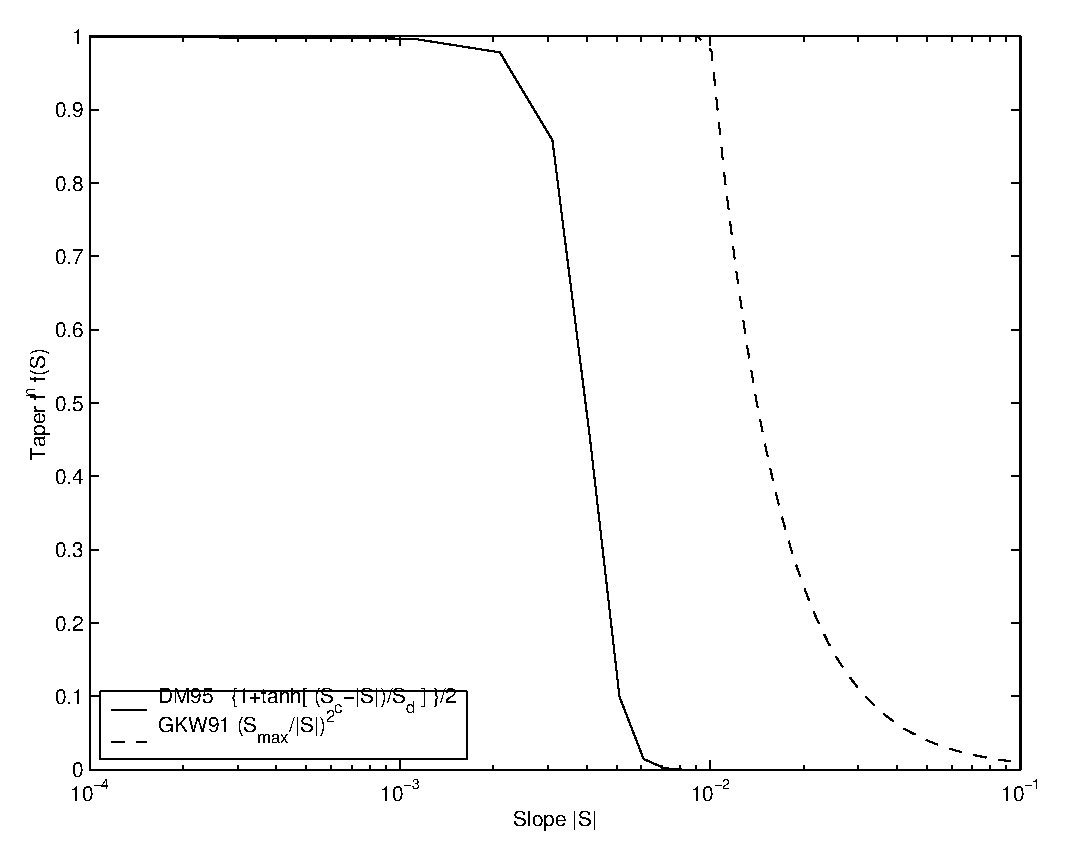
\includegraphics{part6/tapers.eps}}
\end{center}
\caption{Taper functions used in GKW99 and DM95.}
\label{fig:tapers}
\end{figure}

\begin{figure}
\begin{center}
\resizebox{5.0in}{3.0in}{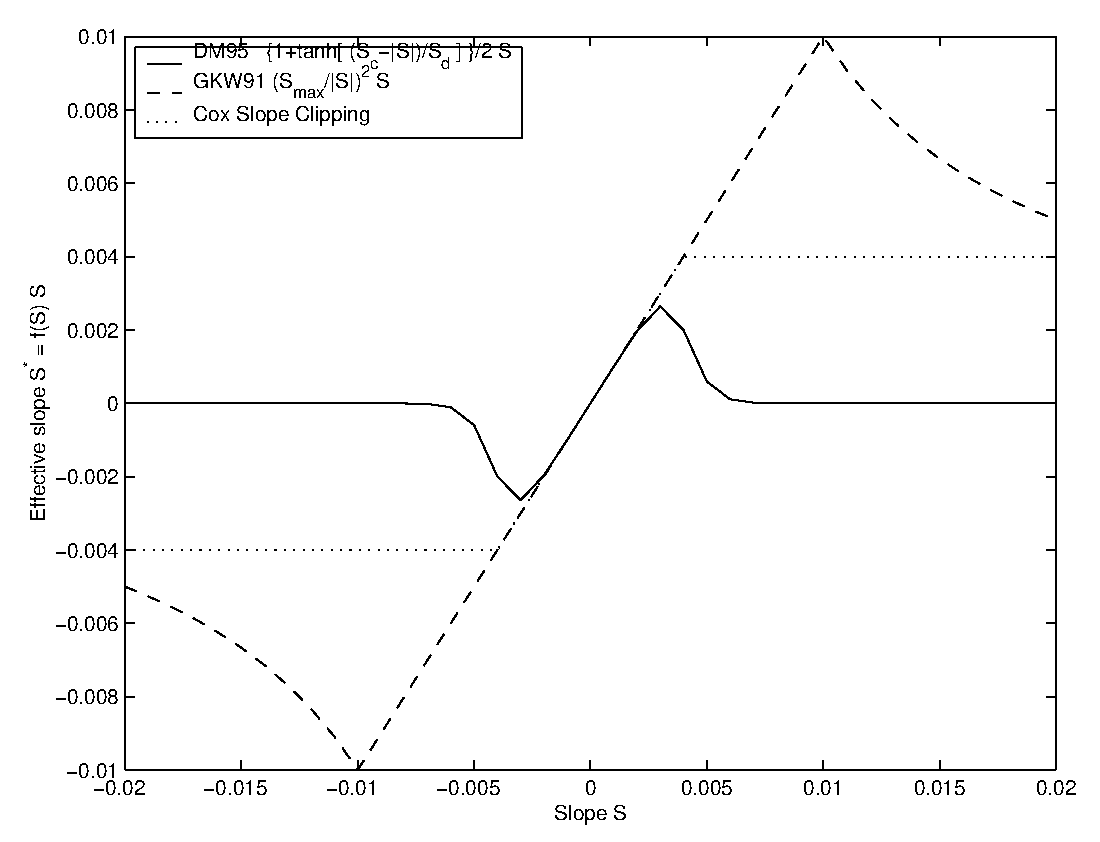
\includegraphics{part6/effective_slopes.eps}}
\end{center}
\caption{Effective slope as a function of ``true'' slope using Cox
slope clipping, GKW91 limiting and DM95 limiting.}
\label{fig:effective_slopes}
\end{figure}


\subsubsection{Slope clipping}

Deep convection sites and the mixed layer are indicated by
homogenized, unstable or nearly unstable stratification. The slopes in
such regions can be either infinite, very large with a sign reversal
or simply very large. From a numerical point of view, large slopes
lead to large variations in the tensor elements (implying large bolus
flow) and can be numerically unstable. This was first recognized by
Cox, 1987, who implemented ``slope clipping'' in the isopycnal mixing
tensor. Here, the slope magnitude is simply restricted by an upper
limit:
\begin{eqnarray}
|\nabla \sigma| & = & \sqrt{ \sigma_x^2 + \sigma_y^2 } \\
S_{lim} & = & - \frac{|\nabla \sigma|}{ S_{max} }
\;\;\;\;\;\;\;\; \mbox{where $S_{max}$ is a parameter} \\
\sigma_z^\star & = & \min( \sigma_z , S_{lim} ) \\
{[s_x,s_y]} & = & - \frac{ [\sigma_x,\sigma_y] }{\sigma_z^\star}
\end{eqnarray}
Notice that this algorithm assumes stable stratification through the
``min'' function. In the case where the fluid is well stratified ($\sigma_z < S_{lim}$) then the slopes evaluate to:
\begin{equation}
{[s_x,s_y]} = - \frac{ [\sigma_x,\sigma_y] }{\sigma_z}
\end{equation}
while in the limited regions ($\sigma_z > S_{lim}$) the slopes become:
\begin{equation}
{[s_x,s_y]} = \frac{ [\sigma_x,\sigma_y] }{|\nabla \sigma|/S_{max}}
\end{equation}
so that the slope magnitude is limited $\sqrt{s_x^2 + s_y^2} =
S_{max}$.

The slope clipping scheme is activated in the model by setting {\bf
GM\_tap\-er\_scheme = 'clipping'} in {\em data.gmredi}.

Even using slope clipping, it is normally the case that the vertical
diffusion term (with coefficient $\kappa_\rho{\bf K}_{33} =
\kappa_\rho S_{max}^2$) is large and must be time-stepped using an
implicit procedure (see section on discretisation and code later).
Fig. \ref{fig-mixedlayer} shows the mixed layer depth resulting from
a) using the GM scheme with clipping and b) no GM scheme (horizontal
diffusion). The classic result of dramatically reduced mixed layers is
evident. Indeed, the deep convection sites to just one or two points
each and are much shallower than we might prefer. This, it turns out,
is due to the over zealous re-stratification due to the bolus transport
parameterization. Limiting the slopes also breaks the adiabatic nature
of the GM/Redi parameterization, re-introducing diabatic fluxes in
regions where the limiting is in effect.

\subsubsection{Tapering: Gerdes, Koberle and Willebrand, Clim. Dyn. 1991}

The tapering scheme used in Gerdes et al., 1999, (\cite{gkw:99})
addressed two issues with the clipping method: the introduction of
large vertical fluxes in addition to convective adjustment fluxes is
avoided by tapering the GM/Redi slopes back to zero in
low-stratification regions; the adjustment of slopes is replaced by a
tapering of the entire GM/Redi tensor. This means the direction of
fluxes is unaffected as the amplitude is scaled.

The scheme inserts a tapering function, $f_1(S)$, in front of the
GM/Redi tensor:
\begin{equation}
f_1(S) = \min \left[ 1, \left( \frac{S_{max}}{|S|}\right)^2 \right]
\end{equation}
where $S_{max}$ is the maximum slope you want allowed. Where the
slopes, $|S|<S_{max}$ then $f_1(S) = 1$ and the tensor is un-tapered
but where $|S| \ge S_{max}$ then $f_1(S)$ scales down the tensor so
that the effective vertical diffusivity term $\kappa f_1(S) |S|^2 =
\kappa S_{max}^2$.

The GKW tapering scheme is activated in the model by setting {\bf
GM\_tap\-er\_scheme = 'gkw91'} in {\em data.gmredi}.

\subsection{Tapering: Danabasoglu and McWilliams, J. Clim. 1995}

The tapering scheme used by Danabasoglu and McWilliams, 1995,
\cite{dm:95}, followed a similar procedure but used a different
tapering function, $f_1(S)$:
\begin{equation}
f_1(S) = \frac{1}{2} \left( 1+\tanh \left[ \frac{S_c - |S|}{S_d} \right] \right)
\end{equation}
where $S_c = 0.004$ is a cut-off slope and $S_d=0.001$ is a scale over
which the slopes are smoothly tapered. Functionally, the operates in
the same way as the GKW91 scheme but has a substantially lower
cut-off, turning off the GM/Redi SGS parameterization for weaker
slopes.

The DM tapering scheme is activated in the model by setting {\bf
GM\_tap\-er\_scheme = 'dm95'} in {\em data.gmredi}.

\subsection{Tapering: Large, Danabasoglu and Doney, JPO 1997}

The tapering used in Large et al., 1997, \cite{ldd:97}, is based on the
DM95 tapering scheme, but also tapers the scheme with an additional
function of height, $f_2(z)$, so that the GM/Redi SGS fluxes are
reduced near the surface:
\begin{equation}
f_2(S) = \frac{1}{2} \left( 1 + \sin(\pi \frac{z}{D} - \pi/2)\right)
\end{equation}
where $D = L_\rho |S|$ is a depth-scale and $L_\rho=c/f$ with
$c=2$~m~s$^{-1}$.  This tapering with height was introduced to fix
some spurious interaction with the mixed-layer KPP parameterization.

The LDD tapering scheme is activated in the model by setting {\bf
GM\_tap\-er\_scheme = 'ldd97'} in {\em data.gmredi}.




\begin{figure}
\begin{center}
%\includegraphics{mixedlayer-cox.eps}
%\includegraphics{mixedlayer-diff.eps}
Figure missing.
\end{center}
\caption{Mixed layer depth using GM parameterization with a) Cox slope
clipping and for comparison b) using horizontal constant diffusion.}
\label{fig-mixedlayer}
\end{figure}






\newpage
\subsection{KPP Package: Ocean vertical mixing -- 
the nonlocal K-profile parameterization scheme}

\label{sec:pkg:kpp}
\begin{rawhtml}
<!-- CMIREDIR:package_kpp: -->
\end{rawhtml}


\newpage
% \documentclass[12pt]{article}
% \usepackage{amssymb}
% 
% \usepackage{graphics}
% 
% 
% \oddsidemargin -4mm \evensidemargin 0mm
% \textwidth 165mm
% \textheight 230mm
% \topmargin -2mm \headsep -2mm
% \renewcommand{\baselinestretch}{1.5}
% \begin{document}
% 

%%%--------------------------------------%%%
\def\deg{$^o$}
\section{BULK\_FORCE: Bulk Formula Package}
\label{sec:pkg:bulk_formula}
\begin{rawhtml}
<!-- CMIREDIR:package_bulk_formula: -->
\end{rawhtml}

author: Stephanie Dutkiewicz\\

\noindent
Instead of forcing the model with heat and fresh water flux data,
this package calculates these fluxes using the changing sea surface
temperature. We need to read in some atmospheric data:
{\bf air temperature, air humidity, down shortwave radiation,
     down longwave radiation, precipitation, wind speed}.
The current setup also reads in {\bf wind stress}, but this
can be changed so that the stresses are calculated from the
wind speed.

The current setup requires that there is the thermodynamic-seaice package
({\it pkg/thsice}, also refered below as seaice)
is also used. It would be useful though to have it also
setup to run with some very simple parametrization of the sea ice.

%%%%%%%%%%%%%%%%%%%%%%%%%%%%%%%%%%%%%%%%%%%%%%%%%%%%%%%%%%%%%%

\vspace{1cm}

\noindent
The heat and fresh water fluxes are calculated in {\it bulkf\_forcing.F}
called from {\it forward\_step.F}. These fluxes are used over open water,
fluxes over seaice are recalculated in the sea-ice package.
Before the call to {\it bulkf\_forcing.F} we call 
{\it bulkf\_fields\_load.F} to find the current atmospheric conditions.
The only other changes to the model code come from the initializing
and writing diagnostics of these fluxes.

%%%%%%%%%%%%%%%%%%%%%%%%%%%%%%%%%%%%%%%%%%%%%%%%%%%%%%%%%%%%%%
\vspace{1cm}
\noindent
{\bf \underline{subroutine BULKF\_FIELDS\_LOAD}}

\noindent
Here we find the atmospheric data needed for the bulk formula
calculations. These are read in at periodic intervals and
values are interpolated to the current time. The data file names
come from {\bf data.blk}. The values that can be read in are:
air temperature, air humidity, precipitation, 
down solar radiation, down long
wave radiation, zonal and meridional wind speeds, total wind
speed, net heat flux, net freshwater forcing, cloud cover,
snow fall, zonal and meridional wind stresses, and SST and SSS
used for relaxation terms.
Not all these files are necessary or used. For instance cloud
cover and snow fall are not used in the current bulk formula
calculation. If total wind speed is not supplied, wind speed
is calculate from the zonal and meridional components. If
wind stresses are not read in, then the stresses are calculated
from the wind speed. Net heat flux and net freshwater can be
read in and used over open ocean instead of the bulk formula
calculations (but over seaice the bulkf formula is always
used). This is "hardwired" into {\it bulkf\_forcing} and
the "ch" in the variable names suggests that this is "cheating".
SST and SSS need to be read in if there is any relaxation used.


%%%%%%%%%%%%%%%%%%%%%%%%%%%%%%%%%%%%%%%%%%%%%%%%%%%%%%%%%%%%%%


\vspace{1cm}
\noindent
{\bf \underline{subroutine BULKF\_FORCING}}

\noindent
In {\it bulkf\_forcing.F}, we calculate  heat and fresh water
fluxes (and wind stress, if necessary) for each grid cell.
First we determine if the grid cell is open water or seaice
and this information is carried by {\bf iceornot}. There is
a provision here for a different designation if there is
snow cover (but currently this does not make any difference).
We then call {\it bulkf\_formula\_lanl.F} which provides
values for: up long wave radiation, latent and sensible heat
fluxes, the derivative of these three with respect to surface
temperature, wind stress, evaporation. 
Net long wave radiation is calculated from the combination
of the down long wave read in and the up long wave calculated.

We then find the albedo of the surface - with a call to
{\it sfc\_albedo} if there is sea-ice (see the seaice package
for information on the subroutine). If the grid cell is open
ocean the albedo is set as 0.1. Note that this is a parameter
that can be used to tune the results. The net short wave
radiation is then the down shortwave radiation minus the 
amount reflected.

If the wind stress needed to be calculated in {\it bulkf\_formula\_lanl.F},
it was calculated to grid cell center points, so in {\it bulkf\_forcing.F}
we regrid to {\bf u} and {\bf v} points. We let the model know
if it has read in stresses or calculated stresses by the switch
{\bf readwindstress} which is can be set in data.blk, and defaults
to {\bf .TRUE.}.

We then calculate {\bf Qnet} and {\bf EmPmR} that will be used
as the fluxes over the open ocean. There is a provision for
using runoff. If we are "cheating" and using observed fluxes 
over the open ocean, then there is a provision here to
use read in {\bf Qnet} and {\bf EmPmR}.

The final call is to calculate averages of the terms found
in this subroutine.

%%%%%%%%%%%%%%%%%%%%%%%%%%%%%%%%%%%%%%%%%%%%%%%%%%%%%%%%%%%%%%
\vspace{1cm}
\noindent
{\bf {\underline{ subroutine BULKF\_FORMULA\_LANL}}}

\noindent
This is the main program of the package where the
heat fluxes and freshwater fluxes over ice and
open water are calculated. Note that this subroutine
is also called from the seaice package during the
iterations to find the ice surface temperature.

Latent heat ($L$) used in this subroutine 
depends on the state of the surface: vaporization for
open water, fusion and vaporization for ice surfaces.
Air temperature is converted from Celsius to Kelvin.
If there is no wind speed ($u_s$) given, then the wind speed
is calculated from the zonal and meridional components.

We calculate the virtual temperature:
\[
T_o = T_{air} (1+\gamma q_{air})
\]
where $T_{air}$ is the air temperature at $h_T$, $q_{air}$ is
humidity at $h_q$ and $\gamma$ is a constant.

The saturated vapor pressure is calculate (QQ ref):
\[
q_{sat} = \frac{a}{p_o} e^{L (b-\frac{c}{T_{srf}})}
\]
where $a,b,c$ are constants, $T_{srf}$ is surface temperature
and $p_o$ is the surface pressure.

The two values crucial for the bulk formula calculations are
the difference between air at sea surface and sea surface temperature:
\[
\Delta T = T_{air} - T_{srf} +\alpha h_T
\]
where $\alpha$ is adiabatic lapse rate and $h_T$ is the  height
where the air temperature was taken; and the difference
between the air humidity and the saturated humidity
\[
\Delta q = q_{air} - q_{sat}.
\]

We then calculate the turbulent exchange coefficients
following Bryan et al (1996) and the numerical scheme
of Hunke and Lipscombe (1998). 
We estimate initial values for the exchange coefficients, $c_u$,
$c_T$ and $c_q$ as
\[
\frac{\kappa}{ln(z_{ref}/z_{rou})}
\]
where $\kappa$ is the Von Karman constant, $z_{ref}$ is a
reference height and $z_{rou}$ is a roughness length scale
which could be a function of type of surface, but is here set
as a constant. Turbulent scales are:
\begin{eqnarray}
u^* & = & c_u u_s \nonumber\\
T^* & = & c_T \Delta T \nonumber\\
q^* & = & c_q \Delta q \nonumber
\end{eqnarray}

We find the "integrated flux profile" for momentum and stability
if there are stable QQ conditions ($\Upsilon>0$) :
\[
\psi_m = \psi_s = -5 \Upsilon
\]
and for unstable QQ conditions ($\Upsilon<0$):
\begin{eqnarray}
\psi_m & = & 2 ln(0.5(1+\chi)) + ln(0.5(1+\chi^2)) - 2 \tan^{-1} \chi + \pi/2
\nonumber \\
\psi_s & = & 2 ln(0.5(1+\chi^2)) \nonumber
\end{eqnarray}
where
\[
\Upsilon = \frac{\kappa g z_{ref}}{u^{*2}} (\frac{T^*}{T_o} + 
\frac{q^*}{1/\gamma + q_a})
\]
and $\chi=(1-16\Upsilon)^{1/2}$.

The coefficients are updated through 5 iterations as:
\begin{eqnarray}
c_u & = & \frac {\hat{c_u}}{1+\hat{c_u}(\lambda - \psi_m)/\kappa} \nonumber \\
c_T & = & \frac {\hat{c_T}}{1+\hat{c_T}(\lambda - \psi_s)/\kappa} \nonumber \\
c_q & = & c'_T
\end{eqnarray}
where $\lambda =ln(h_T/z_{ref})$.

We can then find the bulk formula heat fluxes:

\vspace{.2cm}
\noindent
Sensible heat flux:
\[
Q_s=\rho_{air} c_{p_{air}} u_s c_u c_T \Delta T
\]

\vspace{.2cm}
\noindent
Latent heat flux:
\[
Q_l=\rho_{air} L u_s c_u c_q \Delta q
\]

\vspace{.2cm}
\noindent
Up long wave radiation
\[
Q_{lw}^{up}=\epsilon \sigma T_{srf}^4
\]
where $\epsilon$ is emissivity (which can be different for
open ocean, ice and snow), $\sigma$ is Stefan-Boltzman constant.

We calculate the derivatives of the three above functions
with respect to surface temperature
\begin{eqnarray}
\frac{dQ_s}{d_T} & = & \rho_{air} c_{p_{air}} u_s c_u c_T \nonumber \\
\frac{dQ_l}{d_T} & = & \frac{\rho_{air} L^2 u_s c_u c_q c}{T_{srf}^2} \nonumber \\
\frac{dQ_{]lw}^{up}}{d_T} & = &  4 \epsilon \sigma t_{srf}^3 \nonumber
\end{eqnarray}

And total derivative $\frac{dQ_o}{dT}= \frac{dQ_s}{dT} +
\frac{dQ_l}{dT} + \frac{dQ_{lw}^{up}}{dT}$.




If we do not read in the wind stress, it is calculated here.

%%%%%%%%%%%%%%%%%%%%%%%%%%%%%%%%%%%%%%%%%%%%%%%%%%%%%%%%%%%%%%%

\vspace{1cm}

\noindent
{\bf {\underline{Initializing subroutines}}}

\noindent
{\it bulkf\_init.F}:
Set bulkf variables to zero.

\noindent
{\it bulkf\_readparms.F}:
Reads {\bf data.blk}

%%%%%%%%%%%%%%%%%%%%%%%%%%%%%%%%%%%%%%%%%%%%%%%%%%%%%%%%%%%%%%%

\vspace{1cm}

\noindent
{\bf {\underline{Diagnostic subroutines}}}

\noindent
{\it bulkf\_ave.F}:
Keeps track of means of the bulkf variables

\noindent
{\it bulkf\_diags.F}:
Finds averages and writes out diagnostics

%%%%%%%%%%%%%%%%%%%%%%%%%%%%%%%%%%%%%%%%%%%%%%%%%%%%%%%%%%%%%%%%
\vspace{1cm}

\noindent
{\bf {\underline{Common Blocks}}}

\noindent
{\it BULKF.h}: BULKF Variables,  data file names, and logicals
{\bf readwindstress} and {\bf readsurface}

\noindent
{\it BULKF\_DIAGS.h}: matrices for diagnostics: averages of fields
from {\it bulkf\_diags.F}

\noindent
{\it BULKF\_ICE\_CONSTANTS.h}: 
all the parameters need by the ice model and in the bulkf formula
calculations.

%%%%%%%%%%%%%%%%%%%%%%%%%%%%%%%%%%%%%%%%%%%%%%%%%%%%%%%%%%%%%%%%%%
\vspace{1cm}

\noindent
{\bf {\underline{Input file DATA.ICE}}}

\noindent
We read in the file names of atmospheric data used in
the  bulk formula calculations. Here we can also set
the logicals: {\bf readwindstress} if we read in the
wind stress rather than calculate it from the wind
speed; and {\bf readsurface} to read in the surface
temperature and salinity if these will be used as
part of a relaxing term.

%%%%%%%%%%%%%%%%%%%%%%%%%%%%%%%%%%%%%%%%%%%%%%%%%%%%%%%%%%%%
\vspace{1cm}

\noindent
{\bf {\underline{Important Notes}}}

\noindent
{\bf 1)} heat fluxes have different signs in the ocean and ice
models.

\noindent
{\bf 2)} {\bf StartIceModel} must be changed in {\bf data.ice}:
1 (if starting from no ice), 0 (if using pickup.ic file).

%%%%%%%%%%%%%%%%%%%%%%%%%%%%%%%%%%%%%%%%%%%%%%%%%%%%%%%%%%%%%%

\vspace{1cm}

\noindent 
{\bf {\underline{References}}}


\vspace{.2cm}

\noindent
Bryan F.O., B.G Kauffman, W.G. Large, P.R. Gent, 1996:
The NCAR CSM flux coupler. Technical note TN-425+STR,
NCAR.

\vspace{.2cm}

\noindent
Hunke, E.C and W.H. Lipscomb, circa 2001: CICE: the Los Alamos
Sea Ice Model Documentation and Software User's Manual.
LACC-98-16v.2.\\
(note: this documentation is no longer available as CICE has progressed
to a very different version 3)





%%%%%%%%%%%%%%%%%%%%%%%%%%%%%%%%%%%%%%%%%%%
% \end{document}


\newpage
\section{The external forcing package \texttt{exf}
\label{sectionexf}}
\begin{rawhtml}
<!-- CMIREDIR:sectionexf: -->
\end{rawhtml}

\subsection{Summary}

{\footnotesize
\begin{verbatim}
c     Field definitions, units, and sign conventions:
c     ===============================================
c
c     ustress   :: Zonal surface wind stress in N/m^2
c                  > 0 for increase in uVel, which is west to
c                      east for cartesian and spherical polar grids
c                  Typical range: -0.5 < ustress < 0.5
c                  Southwest C-grid U point
c                  Input field
c
c     vstress   :: Meridional surface wind stress in N/m^2
c                  > 0 for increase in vVel, which is south to
c                      north for cartesian and spherical polar grids
c                  Typical range: -0.5 < vstress < 0.5
c                  Southwest C-grid V point
c                  Input field
c
c     hflux     :: Net upward surface heat flux excluding shortwave in W/m^2
c                  hflux = latent + sensible + lwflux
c                  > 0 for decrease in theta (ocean cooling)
c                  Typical range: -250 < hflux < 600
c                  Southwest C-grid tracer point
c                  Input field
c
c     sflux     :: Net upward freshwater flux in m/s
c                  sflux = evap - precip - runoff
c                  > 0 for increase in salt (ocean salinity)
c                  Typical range: -1e-7 < sflux < 1e-7
c                  Southwest C-grid tracer point
c                  Input field
c
c     swflux    :: Net upward shortwave radiation in W/m^2
c                  swflux = - ( swdown - ice and snow absorption - reflected )
c                  > 0 for decrease in theta (ocean cooling)
c                  Typical range: -350 < swflux < 0
c                  Southwest C-grid tracer point
c                  Input field
c
c     uwind     :: Surface (10-m) zonal wind velocity in m/s
c                  > 0 for increase in uVel, which is west to
c                      east for cartesian and spherical polar grids
c                  Typical range: -10 < uwind < 10
c                  Southwest C-grid U point
c                  Input or input/output field
c
c     vwind     :: Surface (10-m) meridional wind velocity in m/s
c                  > 0 for increase in vVel, which is south to
c                      north for cartesian and spherical polar grids
c                  Typical range: -10 < vwind < 10
c                  Southwest C-grid V point
c                  Input or input/output field
c
c     atemp     :: Surface (2-m) air temperature in deg K
c                  Typical range: 200 < atemp < 300
c                  Southwest C-grid tracer point
c                  Input or input/output field
c
c     aqh       :: Surface (2m) specific humidity in kg/kg
c                  Typical range: 0 < aqh < 0.02
c                  Southwest C-grid tracer point
c                  Input or input/output field
c
c     lwflux    :: Net upward longwave radiation in W/m^2
c                  lwflux = - ( lwdown - ice and snow absorption - emitted )
c                  > 0 for decrease in theta (ocean cooling)
c                  Typical range: -20 < lwflux < 170
c                  Southwest C-grid tracer point
c                  Input field
c
c     evap      :: Evaporation in m/s
c                  > 0 for increase in salt (ocean salinity)
c                  Typical range: 0 < evap < 2.5e-7
c                  Southwest C-grid tracer point
c                  Input, input/output, or output field
c
c     precip    :: Precipitation in m/s
c                  > 0 for decrease in salt (ocean salinity)
c                  Typical range: 0 < precip < 5e-7
c                  Southwest C-grid tracer point
c                  Input or input/output field
c
c     runoff    :: River and glacier runoff in m/s
c                  > 0 for decrease in salt (ocean salinity)
c                  Typical range: 0 < runoff < ????
c                  Southwest C-grid tracer point
c                  Input or input/output field
c                  !!! WATCH OUT: Default exf_inscal_runoff !!!
c                  !!! in exf_readparms.F is not 1.0        !!!
c
c     swdown    :: Downward shortwave radiation in W/m^2
c                  > 0 for increase in theta (ocean warming)
c                  Typical range: 0 < swdown < 450
c                  Southwest C-grid tracer point
c                  Input/output field
c
c     lwdown    :: Downward longwave radiation in W/m^2
c                  > 0 for increase in theta (ocean warming)
c                  Typical range: 50 < lwdown < 450
c                  Southwest C-grid tracer point
c                  Input/output field
c
c     apressure :: Atmospheric pressure field in N/m^2
c                  > 0 for ????
c                  Typical range: ???? < apressure < ????
c                  Southwest C-grid tracer point
c                  Input field
C
C
c     NOTES:
c     ======
c
c     Input and output units and sign conventions can be customized
c     using variables exf_inscal_* and exf_outscal_*, which are set
c     by exf_readparms.F
c
c     Output fields fu, fv, Qnet, Qsw, and EmPmR are
c     defined in FFIELDS.h
c
c     #ifndef SHORTWAVE_HEATING, hflux includes shortwave,
c     that is, hflux = latent + sensible + lwflux +swflux
c
c     If (EXFwindOnBgrid .EQ. .TRUE.), uwind and vwind are
c     defined on northeast B-grid U and V points, respectively.
c
c     Arrays *0 and *1 below are used for temporal interpolation.
\end{verbatim}
}



\newpage
\subsection{CAL: The calendar package
\label{sectioncal}}
\begin{rawhtml}
<!-- CMIREDIR:sectioncal: -->
\end{rawhtml}

Authors: Christian Eckert and Patrick Heimbach

This calendar tool was originally intended to enable the use of
absolute dates (Gregorian Calendar dates) in the ocean general
circulation model MITgcmuv. There is, however, a fair amount of
routines that can be used independently of the MITgcmuv. After
some minor modifications the whole package can be used either
as a stand-alone calendar or in connection with any dynamical
model that needs calendar dates. Some straightforward extensions
are still pending e.g. the availability of the Julian Calendar,
to be able to resolve fractions of a second, and to have a time-
step that is longer than one day.

\subsubsection{Basic assumptions for the calendar tool}

    It is assumed that the SMALLEST TIME INTERVAL to be resolved is
    ONE SECOND.

    Further assumptions are that there is an INTEGER NUMBER OF
    MODEL STEPS EACH DAY, and that AT LEAST ONE STEP EACH DAY is
    made.

    Not each individual routine depends on these assumptions; there
    are only a few places where they enter.

\subsubsection{Format of calendar dates}

    In this calendar tool a complete date specification is defined
    as the following integer array:

\begin{verbatim}
c           integer date(4)
c
c           ( yyyymmdd, hhmmss, leap_year, dayofweek )
c
c             date(1) = yyyymmdd    <-- Year-Month-Day
c             date(2) =   hhmmss    <-- Hours-Minutes-Seconds
c             date(3) = leap_year   <-- Leap Year/No Leap Year
c             date(4) = dayofweek   <-- Day of the Week
c
c             leap_year is either equal to 1 (normal year)
c                              or equal to 2 (leap year)
c
c             dayofweek has a range of 1 to 7.
\end{verbatim}

          In case the Gregorian Calendar is used, the first
          day of the week is Friday, since day of the Gregorian
          Calendar was Friday, 15 Oct. 1582. As a date array
          this date would be specified as

\begin{verbatim}
c               refdate(1) = 15821015
c               refdate(2) =        0
c               refdate(3) =        1
c               refdate(4) =        1
\end{verbatim}

\subsubsection{Calendar dates and time intervals}

    Subtracting calendar dates yields time intervals.
    Time intervals have the following format:

\begin{verbatim}
c         integer datediff(4)
c
c           datediff(1) = # Days
c           datediff(2) = hhmmss
c           datediff(3) =      0
c           datediff(4) =     -1
\end{verbatim}

    Such time intervals can be added to or can be subtracted from
    calendar dates. Time intervals can be added to and be
    subtracted from each other.

\subsubsection{Using the calendar together with MITgcm}

    Each routine has as an argument the thread number that it is
    belonging to, even if this number is not used in the routine
    itself.

    In order to include the calendar tool into the MITgcm
    setup the MITgcm subroutine "initialise.F" or the routine
    "initilise\_fixed.F", depending on the MITgcm release, has
    to be modified in the following way:

{\footnotesize
\begin{verbatim}
c         #ifdef ALLOW_CALENDAR
c         C--   Initialise the calendar package.
c         #ifdef USE_CAL_NENDITER
c               CALL cal_Init(
c              I               startTime,
c              I               endTime,
c              I               deltaTclock,
c              I               nIter0,
c              I               nEndIter,
c              I               nTimeSteps,
c              I               myThid
c              &             )
c         #else
c               CALL cal_Init(
c              I               startTime,
c              I               endTime,
c              I               deltaTclock,
c              I               nIter0,
c              I               nTimeSteps,
c              I               myThid
c              &             )
c         #endif
c               _BARRIER
c         #endif
\end{verbatim}
}

    It is useful to have the CPP flag ALLOW\_CALENDAR in
    order to switch from the usual MITgcm setup to the
    one that includes the calendar tool. The CPP flag
    USE\_CAL\_NENDITER has been introduced in order to enable
    the use of the calendar for MITgcm releases earlier
    than checkpoint 25 which do not have the global variable
    *nEndIter*.

\subsubsection{The individual calendars}

Simple model calendar:

          This calendar can be used by defining

\begin{verbatim}
c                  TheCalendar='model'
\end{verbatim}

          in the calendar's data file "data.cal".

          In this case a year is assumed to have 360 days. The
          model year is divided into 12 months with 30 days each.

Gregorian Calendar:

          This calendar can be used by defining

\begin{verbatim}
c                  TheCalendar='gregorian'
\end{verbatim}

          in the calendar's data file "data.cal".

\subsubsection{Short routine description}

{\footnotesize
\begin{verbatim}
c      o  cal_Init          - Initialise the calendar. This is the interface
c                             to the MITgcm.
c
c      o  cal_Set           - Sets the calendar according to the user
c                             specifications.
c
c      o  cal_GetDate       - Given the model's current timestep or the
c                             model's current time return the corresponding
c                             calendar date.
c
c      o  cal_FullDate      - Complete a date specification (leap year and
c                             day of the week).
c
c      o  cal_IsLeap        - Determine whether a given year is a leap year.
c
c      o  cal_TimePassed    - Determine the time passed between two dates.
c
c      o  cal_AddTime       - Add a time interval either to a time interval
c                             or to a date.
c
c      o  cal_TimeInterval  - Given a time interval return the corresponding
c                             date array.
c
c      o  cal_SubDates      - Determine the time interval between two dates
c                             or between two time intervals.
c
c      o  cal_ConvDate      - Decompose a date array or a time interval
c                             array into its components.
c
c      o  cal_CopyDate      - Copy a date array or a time interval array to
c                             another array.
c
c      o  cal_CompDates     - Compare two calendar dates or time intervals. 
c
c      o  cal_ToSeconds     - Given a time interval array return the number
c                             of seconds.
c
c      o  cal_WeekDay       - Return the weekday as a string given the
c                             calendar date.
c
c      o  cal_NumInts       - Return the number of time intervals between two
c                             given dates.
c
c      o  cal_StepsPerDay   - Given an iteration number or the current
c                             integration time return the number of time
c                             steps to integrate in the current calendar day.
c
c      o  cal_DaysPerMonth  - Given an iteration number or the current
c                             integration time return the number of days
c                             to integrate in this calendar month.
c
c      o  cal_MonthsPerYear - Given an iteration number or the current
c                             integration time return the number of months
c                             to integrate in the current calendar year.
c
c      o  cal_StepsForDay   - Given the integration day return the number
c                             of steps to be integrated, the first step,
c                             and the last step in the day specified. The
c                             first and the last step refer to the total
c                             number of steps (1, ... , cal_IntSteps).
c
c      o  cal_DaysForMonth  - Given the integration month return the number
c                             of days to be integrated, the first day,
c                             and the last day in the month specified. The
c                             first and the last day refer to the total
c                             number of steps (1, ... , cal_IntDays).
c
c      o  cal_MonthsForYear - Given the integration year return the number
c                             of months to be integrated, the first month,
c                             and the last month in the year specified. The
c                             first and the last step refer to the total
c                             number of steps (1, ... , cal_IntMonths).
c
c      o  cal_Intsteps      - Return the number of calendar years that are
c                             affected by the current integration.
c
c      o  cal_IntDays       - Return the number of calendar days that are
c                             affected by the current integration.
c
c      o  cal_IntMonths     - Return the number of calendar months that are
c                             affected by the current integration.
c
c      o  cal_IntYears      - Return the number of calendar years that are
c                             affected by the current integration.
c
c      o  cal_nStepDay      - Return the number of time steps that can be
c                             performed during one calendar day.
c
c      o  cal_CheckDate     - Do some simple checks on a date array or on a
c                             time interval array.
c
c      o  cal_PrintError    - Print error messages according to the flags
c                             raised by the calendar routines.
c
c      o  cal_PrintDate     - Print a date array in some format suitable for
c                             the MITgcmuv's protocol output.
c
c      o  cal_TimeStamp     - Given the time and the iteration number return
c                             the date and print all the above numbers.
c
c      o  cal_Summary       - List all the setttings of the calendar tool.
\end{verbatim}
}



\section{Atmosphere Packages}
\newpage
\subsection{Atmospheric Intermediate Physics: AIM}
\label{sec:pkg:aim}
\begin{rawhtml}
<!-- CMIREDIR:package_aim: -->
\end{rawhtml}

Note:
 The folowing document below describes the \texttt{aim\_v23} package
 that is based on the version v23 of the SPEEDY code (\cite{molteni:03}).

\subsubsection{Key subroutines, parameters and files}
\label{sec:pkg:aim:implementation}


\newpage
\section{Land package}

This package provides a simple land model
based on Rong Zhang [e-mail:roz@gfdl.noaa.gov] 2 layers model
(see documentation below).

It is primarily implemented for AIM (\_v23) atmospheric physics
but could be adapted to work with a different atmospheric physics.
Two subroutines ({\it aim\_aim2land.F} {\it aim\_land2aim.F}
in {\it pkg/aim\_v23}) are used as interface with AIM physics. 

Number of layers is a parameter ({\it land\_nLev} in {\it LAND\_SIZE.h})
and can be changed. 

%---------------------------------------------------------------------

% \documentclass[12pt,thmsa]{article}

% \begin{document}

\begin{center}
{\bf Note on Land Model}\\
date: June 1999\\
author: Rong Zhang\\
\end{center}

% \baselineskip19pt

This is a simple 2-layer land model. The top layer depth $z1=0.1m$, the
second layer depth $z2=4m$.

Let $T_{g1},T_{g2}$ be the temperature of each layer, $W_{1,}W_{2}$ be the
soil moisture of each layer. The field capacity $f_{1,}$ $f_{2}$ are the
maximum water amount in each layer, so $W_{i}$ is the ratio of available
water to field capacity. $f_{i}=\gamma z_{i},\gamma =0.24$ is the field
capapcity per meter soil$,$ so $f_{1}=0.024m,$ $f_{2}=0.96m.$

The land temperature is determined by total surface downward heat flux $F,$

\begin{equation}
z_{1}C_{1}\frac{dT_{g1}}{dt}=F-\lambda \frac{T_{g1}-T_{g2}}{(z_{1}+z_{2})/2}
\end{equation}

\begin{center}
\begin{equation}
z_{2}C_{2}\frac{dT_{g2}}{dt}=\lambda \frac{T_{g1}-T_{g2}}{(z_{1}+z_{2})/2}
\end{equation}
\end{center}

here $C_{1},C_{2}$ are the heat capacity of each layer , $\lambda $ is the
thermal conductivity, $\lambda =0.42Wm^{-1}K^{-1}.$

\begin{center}
\bigskip 
\begin{equation}
C_{1}=C_{w}W_{1}\gamma +C_{s}
\end{equation}

\begin{equation}
C_{2}=C_{w}W_{2}\gamma +C_{s}
\end{equation}
\end{center}

$C_{w},C_{s}$ are the heat capacity of water and dry soil respectively. $%
C_{w}=4.2\times 10^{6}Jm^{-3}K^{-1},C_{s}=1.13\times 10^{6}Jm^{-3}K^{-1}.$

\bigskip

The soil moisture is determined by precipitation $P(m/s)$,surface
evaporation $E(m/s)$ and runoff $R(m/s).$

\begin{equation}
\frac{dW_{1}}{dt}=\frac{P-E-R}{f_{1}}+\frac{W_{2}-W_{1}}{\tau }
\end{equation}

$\tau =2$ $days$ is the time constant for diffusion of moisture between
layers.

\begin{equation}
\frac{dW_{2}}{dt}=\frac{f_{1}}{f_{2}}\frac{W_{1}-W_{2}}{\tau }
\end{equation}

In the code, $R=0$ gives better result, $W_{1},W_{2}$ are set to be within
[0, 1]. If $W_{1}$ is greater than 1, then let $\delta W_{1}=W_{1}-1,W_{1}=1$
and $W_{2}=W_{2}+p\delta W_{1}\frac{f_{1}}{f_{2}}$, i.e. the runoff of top
layer is put into second layer. $p=0.5$ is the fraction of top layer runoff
that is put into second layer.

The time step is 1 hour, it takes several years to reach equalibrium offline.

\begin{center}
\bigskip
\end{center}

\textbf{References}

Hansen J. et al. Efficient three-dimensional global models for climate
studies: models I and II. \emph{Monthly Weather Review}, vol.111, no.4, pp.
609-62, 1983

% \end{document}


\newpage
\subsection{Fizhi: High-end Atmospheric Physics}
\label{sec:pkg:fizhi}
\begin{rawhtml}
<!-- CMIREDIR:package_fizhi: -->
\end{rawhtml}
%   EPSF.TEX macro file:
%   Written by Tomas Rokicki of Radical Eye Software, 29 Mar 1989.
%   Revised by Don Knuth, 3 Jan 1990.
%   Revised by Tomas Rokicki to accept bounding boxes with no
%      space after the colon, 18 Jul 1990.
%
%   TeX macros to include an Encapsulated PostScript graphic.
%   Works by finding the bounding box comment,
%   calculating the correct scale values, and inserting a vbox
%   of the appropriate size at the current position in the TeX document.
%
%   To use with the center environment of LaTeX, preface the \epsffile
%   call with a \leavevmode.  (LaTeX should probably supply this itself
%   for the center environment.)
%
%   To use, simply say
%   \input epsf           % somewhere early on in your TeX file
%   \epsfbox{filename.ps} % where you want to insert a vbox for a figure
%
%   Alternatively, you can type
%
%   \epsfbox[0 0 30 50]{filename.ps} % to supply your own BB
%
%   which will not read in the file, and will instead use the bounding
%   box you specify.
%
%   The effect will be to typeset the figure as a TeX box, at the
%   point of your \epsfbox command. By default, the graphic will have its
%   `natural' width (namely the width of its bounding box, as described
%   in filename.ps). The TeX box will have depth zero.
%
%   You can enlarge or reduce the figure by saying
%     \epsfxsize=<dimen> \epsfbox{filename.ps}
%   (or
%     \epsfysize=<dimen> \epsfbox{filename.ps})
%   instead. Then the width of the TeX box will be \epsfxsize and its
%   height will be scaled proportionately (or the height will be
%   \epsfysize and its width will be scaled proportiontally).  The
%   width (and height) is restored to zero after each use.
%
%   A more general facility for sizing is available by defining the
%   \epsfsize macro.    Normally you can redefine this macro
%   to do almost anything.  The first parameter is the natural x size of
%   the PostScript graphic, the second parameter is the natural y size
%   of the PostScript graphic.  It must return the xsize to use, or 0 if
%   natural scaling is to be used.  Common uses include:
%
%      \epsfxsize  % just leave the old value alone
%      0pt         % use the natural sizes
%      #1          % use the natural sizes
%      \hsize      % scale to full width
%      0.5#1       % scale to 50% of natural size
%      \ifnum#1>\hsize\hsize\else#1\fi  % smaller of natural, hsize
%
%   If you want TeX to report the size of the figure (as a message
%   on your terminal when it processes each figure), say `\epsfverbosetrue'.
%
\newread\epsffilein    % file to \read
\newif\ifepsffileok    % continue looking for the bounding box?
\newif\ifepsfbbfound   % success?
\newif\ifepsfverbose   % report what you're making?
\newdimen\epsfxsize    % horizontal size after scaling
\newdimen\epsfysize    % vertical size after scaling
\newdimen\epsftsize    % horizontal size before scaling
\newdimen\epsfrsize    % vertical size before scaling
\newdimen\epsftmp      % register for arithmetic manipulation
\newdimen\pspoints     % conversion factor
%
\pspoints=1bp          % Adobe points are `big'
\epsfxsize=0pt         % Default value, means `use natural size'
\epsfysize=0pt         % ditto
%
\def\epsfbox#1{\global\def\epsfllx{72}\global\def\epsflly{72}%
   \global\def\epsfurx{540}\global\def\epsfury{720}%
   \def\lbracket{[}\def\testit{#1}\ifx\testit\lbracket
   \let\next=\epsfgetlitbb\else\let\next=\epsfnormal\fi\next{#1}}%
%
\def\epsfgetlitbb#1#2 #3 #4 #5]#6{\epsfgrab #2 #3 #4 #5 .\\%
   \epsfsetgraph{#6}}%
%
\def\epsfnormal#1{\epsfgetbb{#1}\epsfsetgraph{#1}}%
%
\def\epsfgetbb#1{%
%
%   The first thing we need to do is to open the
%   PostScript file, if possible.
%
\openin\epsffilein=#1
\ifeof\epsffilein\errmessage{I couldn't open #1, will ignore it}\else
%
%   Okay, we got it. Now we'll scan lines until we find one that doesn't
%   start with %. We're looking for the bounding box comment.
%
   {\epsffileoktrue \chardef\other=12
    \def\do##1{\catcode`##1=\other}\dospecials \catcode`\ =10
    \loop
       \read\epsffilein to \epsffileline
       \ifeof\epsffilein\epsffileokfalse\else
%
%   We check to see if the first character is a % sign;
%   if not, we stop reading (unless the line was entirely blank);
%   if so, we look further and stop only if the line begins with
%   `%%BoundingBox:'.
%
          \expandafter\epsfaux\epsffileline:. \\%
       \fi
   \ifepsffileok\repeat
   \ifepsfbbfound\else
    \ifepsfverbose\message{No bounding box comment in #1; using defaults}\fi\fi
   }\closein\epsffilein\fi}%
%
%   Now we have to calculate the scale and offset values to use.
%   First we compute the natural sizes.
%
\def\epsfclipstring{}% do we clip or not?  If so,
\def\epsfclipon{\def\epsfclipstring{ clip}}%
\def\epsfclipoff{\def\epsfclipstring{}}%
%
\def\epsfsetgraph#1{%
   \epsfrsize=\epsfury\pspoints
   \advance\epsfrsize by-\epsflly\pspoints
   \epsftsize=\epsfurx\pspoints
   \advance\epsftsize by-\epsfllx\pspoints
%
%   If `epsfxsize' is 0, we default to the natural size of the picture.
%   Otherwise we scale the graph to be \epsfxsize wide.
%
   \epsfxsize\epsfsize\epsftsize\epsfrsize
   \ifnum\epsfxsize=0 \ifnum\epsfysize=0
      \epsfxsize=\epsftsize \epsfysize=\epsfrsize
      \epsfrsize=0pt
%
%   We have a sticky problem here:  TeX doesn't do floating point arithmetic!
%   Our goal is to compute y = rx/t. The following loop does this reasonably
%   fast, with an error of at most about 16 sp (about 1/4000 pt).
% 
     \else\epsftmp=\epsftsize \divide\epsftmp\epsfrsize
       \epsfxsize=\epsfysize \multiply\epsfxsize\epsftmp
       \multiply\epsftmp\epsfrsize \advance\epsftsize-\epsftmp
       \epsftmp=\epsfysize
       \loop \advance\epsftsize\epsftsize \divide\epsftmp 2
       \ifnum\epsftmp>0
          \ifnum\epsftsize<\epsfrsize\else
             \advance\epsftsize-\epsfrsize \advance\epsfxsize\epsftmp \fi
       \repeat
       \epsfrsize=0pt
     \fi
   \else \ifnum\epsfysize=0
     \epsftmp=\epsfrsize \divide\epsftmp\epsftsize
     \epsfysize=\epsfxsize \multiply\epsfysize\epsftmp   
     \multiply\epsftmp\epsftsize \advance\epsfrsize-\epsftmp
     \epsftmp=\epsfxsize
     \loop \advance\epsfrsize\epsfrsize \divide\epsftmp 2
     \ifnum\epsftmp>0
        \ifnum\epsfrsize<\epsftsize\else
           \advance\epsfrsize-\epsftsize \advance\epsfysize\epsftmp \fi
     \repeat
     \epsfrsize=0pt
    \else
     \epsfrsize=\epsfysize
    \fi
   \fi
%
%  Finally, we make the vbox and stick in a \special that dvips can parse.
%
   \ifepsfverbose\message{#1: width=\the\epsfxsize, height=\the\epsfysize}\fi
   \epsftmp=10\epsfxsize \divide\epsftmp\pspoints
   \vbox to\epsfysize{\vfil\hbox to\epsfxsize{%
      \ifnum\epsfrsize=0\relax
        \special{PSfile=#1 llx=\epsfllx\space lly=\epsflly\space
            urx=\epsfurx\space ury=\epsfury\space rwi=\number\epsftmp
            \epsfclipstring}%
      \else
        \epsfrsize=10\epsfysize \divide\epsfrsize\pspoints
        \special{PSfile=#1 llx=\epsfllx\space lly=\epsflly\space
            urx=\epsfurx\space ury=\epsfury\space rwi=\number\epsftmp\space
            rhi=\number\epsfrsize \epsfclipstring}%
      \fi
      \hfil}}%
\global\epsfxsize=0pt\global\epsfysize=0pt}%
%
%   We still need to define the tricky \epsfaux macro. This requires
%   a couple of magic constants for comparison purposes.
%
{\catcode`\%=12 \global\let\epsfpercent=%\global\def\epsfbblit{%BoundingBox}}%
%
%   So we're ready to check for `%BoundingBox:' and to grab the
%   values if they are found.
%
\long\def\epsfaux#1#2:#3\\{\ifx#1\epsfpercent
   \def\testit{#2}\ifx\testit\epsfbblit
      \epsfgrab #3 . . . \\%
      \epsffileokfalse
      \global\epsfbbfoundtrue
   \fi\else\ifx#1\par\else\epsffileokfalse\fi\fi}%
%
%   Here we grab the values and stuff them in the appropriate definitions.
%
\def\epsfempty{}%
\def\epsfgrab #1 #2 #3 #4 #5\\{%
\global\def\epsfllx{#1}\ifx\epsfllx\epsfempty
      \epsfgrab #2 #3 #4 #5 .\\\else
   \global\def\epsflly{#2}%
   \global\def\epsfurx{#3}\global\def\epsfury{#4}\fi}%
%
%   We default the epsfsize macro.
%
\def\epsfsize#1#2{\epsfxsize}
%
%   Finally, another definition for compatibility with older macros.
%
\let\epsffile=\epsfbox



\subsubsection{Introduction}
The fizhi (high-end atmospheric physics) package includes a collection of state-of-the-art
physical parameterizations for atmospheric radiation, cumulus convection, atmospheric
boundary layer turbulence, and land surface processes. The collection of atmospheric
physics parameterizations were originally used together as part of the GEOS-3
(Goddard Earth Observing System-3) GCM developed at the NASA/Goddard Global Modelling
and Assimilation Office (GMAO).

% *************************************************************************
% *************************************************************************
 
\subsubsection{Equations}

Moist Convective Processes:

\paragraph{Sub-grid and Large-scale Convection}
\label{sec:fizhi:mc}

Sub-grid scale cumulus convection is parameterized using the Relaxed Arakawa
Schubert (RAS) scheme of \cite{moorsz:92}, which is a linearized Arakawa Schubert
type scheme.  RAS predicts the mass flux from an ensemble of clouds.  Each subensemble is identified
by its entrainment rate and level of neutral bouyancy which are determined by the grid-scale properties.

The thermodynamic variables that are used in RAS to describe the grid scale vertical profile are
the dry static energy, $s=c_pT +gz$, and the moist static energy, $h=c_p T + gz + Lq$. 
The conceptual model behind RAS depicts each subensemble as a rising plume cloud, entraining 
mass from the environment during ascent, and detraining all cloud air at the level of neutral 
buoyancy. RAS assumes that the normalized cloud mass flux, $\eta$, normalized by the cloud base 
mass flux, is a linear function of height, expressed as:
\[
\pp{\eta(z)}{z} = \lambda \hspace{0.4cm}or\hspace{0.4cm} \pp{\eta(P^{\kappa})}{P^{\kappa}} = 
-{c_p \over {g}}\theta\lambda
\]
where we have used the hydrostatic equation written in the form:
\[
\pp{z}{P^{\kappa}} = -{c_p \over {g}}\theta
\]

The entrainment parameter, $\lambda$, characterizes a particular subensemble based on its
detrainment level, and is obtained by assuming that the level of detrainment is the level of neutral
buoyancy, ie., the level at which the moist static energy of the cloud, $h_c$, is equal 
to the saturation moist static energy of the environment, $h^*$.  Following \cite{moorsz:92},
$\lambda$ may be written as
\[
\lambda = { {h_B - h^*_D} \over { {c_p \over g} {\int_{P_D}^{P_B}\theta(h^*_D-h)dP^{\kappa}}} } ,
\]

where the subscript $B$ refers to cloud base, and the subscript $D$ refers to the detrainment level.


The convective instability is measured in terms of the cloud work function $A$, defined as the
rate of change of cumulus kinetic energy. The cloud work function is 
related to the buoyancy, or the difference
between the moist static energy in the cloud and in the environment:
\[
A = \int_{P_D}^{P_B} { {\eta \over {1 + \gamma} } 
\left[ {{h_c-h^*} \over {P^{\kappa}}} \right] dP^{\kappa}}
\]

where $\gamma$ is ${L \over {c_p}}\pp{q^*}{T}$ obtained from the Claussius Clapeyron equation,
and the subscript $c$ refers to the value inside the cloud.


To determine the cloud base mass flux, the rate of change of $A$ in time {\em due to dissipation by 
the clouds} is assumed to approximately balance the rate of change of $A$ {\em due to the generation 
by the large scale}. This is the quasi-equilibrium assumption, and results in an expression for $m_B$:
\[
m_B = {{- \left.{dA \over dt} \right|_{ls}} \over K}
\]

where $K$ is the cloud kernel, defined as the rate of change of the cloud work function per
unit cloud base mass flux, and is currently obtained by analytically differentiating the 
expression for $A$ in time.
The rate of change of $A$ due to the generation by the large scale can be written as the
difference between the current $A(t+\Delta t)$ and its equillibrated value after the previous 
convective time step 
$A(t)$, divided by the time step. $A(t)$ is approximated as some critical $A_{crit}$,
computed by Lord (1982) from $in situ$ observations.


The predicted convective mass fluxes are used to solve grid-scale temperature
and moisture budget equations to determine the impact of convection on the large scale fields of
temperature (through latent heating and compensating subsidence) and moisture (through
precipitation and detrainment):
\[
\left.{\pp{\theta}{t}}\right|_{c} = \alpha { m_B \over {c_p P^{\kappa}}} \eta \pp{s}{p}
\]
and
\[
\left.{\pp{q}{t}}\right|_{c} = \alpha { m_B \over {L}} \eta (\pp{h}{p}-\pp{s}{p})
\]
where $\theta = {T \over P^{\kappa}}$, $P = (p/p_0)$, and $\alpha$ is the relaxation parameter.

As an approximation to a full interaction between the different allowable subensembles,
many clouds are simulated frequently, each modifying the large scale environment some fraction
$\alpha$ of the total adjustment. The parameterization thereby ``relaxes'' the large scale environment
towards equillibrium.  

In addition to the RAS cumulus convection scheme, the fizhi package employs a
Kessler-type scheme for the re-evaporation of falling rain (\cite{sudm:88}), which
correspondingly adjusts the temperature assuming $h$ is conserved. RAS in its current
formulation assumes that all cloud water is deposited into the detrainment level as rain.
All of the rain is available for re-evaporation, which begins in the level below detrainment. 
The scheme accounts for some microphysics such as
the rainfall intensity, the drop size distribution, as well as the temperature, 
pressure and relative humidity of the surrounding air.  The fraction of the moisture deficit 
in any model layer into which the rain may re-evaporate is controlled by a free parameter,
which allows for a relatively efficient re-evaporation of liquid precipitate and larger rainout
for frozen precipitation.

Due to the increased vertical resolution near the surface, the lowest model 
layers are averaged to provide a 50 mb thick sub-cloud layer for RAS.  Each time RAS is
invoked (every ten simulated minutes), 
a number of randomly chosen subensembles are checked for the possibility 
of convection, from just above cloud base to 10 mb.  

Supersaturation or large-scale precipitation is initiated in the fizhi package whenever 
the relative humidity in any grid-box exceeds a critical value, currently 100 \%.
The large-scale precipitation re-evaporates during descent to partially saturate 
lower layers in a process identical to the re-evaporation of convective rain. 

 
\paragraph{Cloud Formation}
\label{sec:fizhi:clouds}

Convective and large-scale cloud fractons which are used for cloud-radiative interactions are determined
diagnostically as part of the cumulus and large-scale parameterizations.
Convective cloud fractions produced by RAS are proportional to the 
detrained liquid water amount given by

\[
F_{RAS} = \min\left[ {l_{RAS}\over l_c}, 1.0 \right]
\]

where $l_c$ is an assigned critical value equal to $1.25$ g/kg.
A memory is associated with convective clouds defined by:

\[
F_{RAS}^n = \min\left[ F_{RAS} + (1-{\Delta t_{RAS}\over\tau})F_{RAS}^{n-1}, 1.0 \right]
\]

where $F_{RAS}$ is the instantanious cloud fraction and $F_{RAS}^{n-1}$ is the cloud fraction
from the previous RAS timestep.  The memory coefficient is computed using a RAS cloud timescale,
$\tau$, equal to 1 hour.  RAS cloud fractions are cleared when they fall below 5 \%.

Large-scale cloudiness is defined, following Slingo and Ritter (1985), as a function of relative
humidity:

\[
F_{LS} = \min\left[ { \left( {RH-RH_c \over 1-RH_c} \right) }^2, 1.0 \right]
\]

where

\bqa
RH_c & = & 1-s(1-s)(2-\sqrt{3}+2\sqrt{3} \, s)r \nonumber \\
   s & = & p/p_{surf} \nonumber \\
   r & = & \left( {1.0-RH_{min} \over \alpha} \right) \nonumber \\
RH_{min} & = & 0.75 \nonumber \\
\alpha & = & 0.573285 \nonumber  .
\eqa

These cloud fractions are suppressed, however, in regions where the convective
sub-cloud layer is conditionally unstable.  The functional form of $RH_c$ is shown in
Figure (\ref{fig.rhcrit}).

\begin{figure*}[htbp]
  \vspace{0.4in}
  \centerline{  \epsfysize=4.0in  \epsfbox{part6/rhcrit.ps}}
  \vspace{0.4in}
  \caption  [Critical Relative Humidity for Clouds.]
            {Critical Relative Humidity for Clouds.}
  \label{fig.rhcrit}
\end{figure*}

The total cloud fraction in a grid box is determined by the larger of the two cloud fractions:

\[
F_{CLD} = \max \left[ F_{RAS},F_{LS} \right] .
\]

Finally, cloud fractions are time-averaged between calls to the radiation packages.


Radiation:

The parameterization of radiative heating in the fizhi package includes effects 
from both shortwave and longwave processes.
Radiative fluxes are calculated at each
model edge-level in both up and down directions.
The heating rates/cooling rates are then obtained 
from the vertical divergence of the net radiative fluxes.

The net flux is
\[
F = F^\uparrow - F^\downarrow
\]
where $F$ is the net flux, $F^\uparrow$ is the upward flux and $F^\downarrow$ is
the downward flux.

The heating rate due to the divergence of the radiative flux is given by
\[
\pp{\rho c_p T}{t} = - \pp{F}{z}
\]
or
\[
\pp{T}{t} = \frac{g}{c_p \pi} \pp{F}{\sigma}
\]
where $g$ is the accelation due to gravity
and $c_p$ is the heat capacity of air at constant pressure.
  
The time tendency for Longwave
Radiation is updated every 3 hours.  The time tendency for Shortwave Radiation is updated once
every three hours assuming a normalized incident solar radiation, and subsequently modified at
every model time step by the true incident radiation.  
The solar constant value used in the package is equal to 1365 $W/m^2$
and a $CO_2$ mixing ratio of 330 ppm. 
For the ozone mixing ratio, monthly mean zonally averaged 
climatological values specified as a function
of latitude and height (\cite{rosen:87}) are linearly interpolated to the current time.


\paragraph{Shortwave Radiation}

The shortwave radiation package used in the package computes solar radiative 
heating due to the absoption by water vapor, ozone, carbon dioxide, oxygen,
clouds, and aerosols and due to the
scattering by clouds, aerosols, and gases.
The shortwave radiative processes are described by 
\cite{chou:90,chou:92}. This shortwave package
uses the Delta-Eddington approximation to compute the
bulk scattering properties of a single layer following King and Harshvardhan (JAS, 1986).
The transmittance and reflectance of diffuse radiation
follow the procedures of Sagan and Pollock (JGR, 1967) and \cite{lhans:74}.

Highly accurate heating rate calculations are obtained through the use
of an optimal grouping strategy of spectral bands.  By grouping the UV and visible regions
as indicated in Table \ref{tab:fizhi:solar2}, the Rayleigh scattering and the ozone absorption of solar radiation
can be accurately computed in the ultraviolet region and the photosynthetically
active radiation (PAR) region.
The computation of solar flux in the infrared region is performed with a broadband
parameterization using the spectrum regions shown in Table \ref{tab:fizhi:solar1}.
The solar radiation algorithm used in the fizhi package can be applied not only for climate studies but
also for studies on the photolysis in the upper atmosphere and the photosynthesis in the biosphere.

\begin{table}[htb]
\begin{center}
{\bf UV and Visible Spectral Regions} \\
\vspace{0.1in}
\begin{tabular}{|c|c|c|} 
\hline
Region & Band & Wavelength (micron) \\ \hline
\hline
UV-C   &  1.  &  .175 - .225  \\
       &  2.  &  .225 - .245  \\
       &      &  .260 - .280  \\
       &  3.  &  .245 - .260  \\ \hline
UV-B   &  4.  &  .280 - .295  \\
       &  5.  &  .295 - .310  \\
       &  6.  &  .310 - .320  \\ \hline
UV-A   &  7.  &  .320 - .400  \\ \hline
PAR    &  8.  &  .400 - .700  \\
\hline
\end{tabular}
\end{center}
\caption{UV and Visible Spectral Regions used in shortwave radiation package.}
\label{tab:fizhi:solar2}
\end{table}

\begin{table}[htb]
\begin{center}
{\bf Infrared Spectral Regions} \\
\vspace{0.1in}
\begin{tabular}{|c|c|c|} 
\hline
Band & Wavenumber(cm$^{-1}$) & Wavelength (micron) \\ \hline
\hline
1  &    1000-4400    &    2.27-10.0 \\
2  &    4400-8200    &    1.22-2.27 \\
3  &    8200-14300   &    0.70-1.22 \\
\hline
\end{tabular}
\end{center}
\caption{Infrared Spectral Regions used in shortwave radiation package.}
\label{tab:fizhi:solar1}
\end{table}

Within the shortwave radiation package, 
both ice and liquid cloud particles are allowed to co-exist in any of the model layers. 
Two sets of cloud parameters are used, one for ice paticles and the other for liquid particles.
Cloud parameters are defined as the cloud optical thickness and the effective cloud particle size.
In the fizhi package, the effective radius for water droplets is given as 10 microns,
while 65 microns is used for ice particles.  The absorption due to aerosols is currently
set to zero.

To simplify calculations in a cloudy atmosphere, clouds are
grouped into low ($p>700$ mb), middle (700 mb $\ge p > 400$ mb), and high ($p < 400$ mb) cloud regions. 
Within each of the three regions, clouds are assumed maximally
overlapped, and the cloud cover of the group is the maximum
cloud cover of all the layers in the group.  The optical thickness
of a given layer is then scaled for both the direct (as a function of the
solar zenith angle) and diffuse beam radiation 
so that the grouped layer reflectance is the same as the original reflectance.
The solar flux is computed for each of eight cloud realizations possible within this
low/middle/high classification, and appropriately averaged to produce the net solar flux.

\paragraph{Longwave Radiation}

The longwave radiation package used in the fizhi package is thoroughly described by \cite{chsz:94}.
As described in that document, IR fluxes are computed due to absorption by water vapor, carbon
dioxide, and ozone.  The spectral bands together with their absorbers and parameterization methods,
configured for the fizhi package, are shown in Table \ref{tab:fizhi:longwave}.


\begin{table}[htb]
\begin{center}
{\bf IR Spectral Bands} \\
\vspace{0.1in}
\begin{tabular}{|c|c|l|c| } 
\hline
Band & Spectral Range (cm$^{-1}$) & Absorber & Method \\ \hline
\hline
1   & 0-340      & H$_2$O line      & T \\ \hline
2   & 340-540    & H$_2$O line      & T \\ \hline
3a  & 540-620    & H$_2$O line      & K \\ 
3b  & 620-720    & H$_2$O continuum & S \\ 
3b  & 720-800    & CO$_2$           & T \\ \hline 
4   & 800-980    & H$_2$O line      & K \\ 
    &            & H$_2$O continuum & S \\ \hline 
    &            & H$_2$O line      & K \\ 
5   & 980-1100   & H$_2$O continuum & S \\ 
    &            & O$_3$            & T \\ \hline 
6   & 1100-1380  & H$_2$O line      & K \\ 
    &            & H$_2$O continuum & S \\ \hline
7   & 1380-1900  & H$_2$O line      & T \\ \hline 
8   & 1900-3000  & H$_2$O line      & K \\ \hline 
\hline
\multicolumn{4}{|l|}{ \quad K: {\em k}-distribution method with linear pressure scaling } \\
\multicolumn{4}{|l|}{ \quad T: Table look-up with temperature and pressure scaling } \\
\multicolumn{4}{|l|}{ \quad S: One-parameter temperature scaling } \\
\hline
\end{tabular}
\end{center}
\vspace{0.1in}
\caption{IR Spectral Bands, Absorbers, and Parameterization Method (from \cite{chsz:94})}
\label{tab:fizhi:longwave}
\end{table}


The longwave radiation package accurately computes cooling rates for the middle and 
lower atmosphere from 0.01 mb to the surface.  Errors are $<$ 0.4 C day$^{-1}$ in cooling
rates and $<$ 1\% in fluxes.  From Chou and Suarez, it is estimated that the total effect of 
neglecting all minor absorption bands and the effects of minor infrared absorbers such as
nitrous oxide (N$_2$O), methane (CH$_4$), and the chlorofluorocarbons (CFCs), is an underestimate
of $\approx$ 5 W/m$^2$ in the downward flux at the surface and an overestimate of $\approx$ 3 W/m$^2$
in the upward flux at the top of the atmosphere.

Similar to the procedure used in the shortwave radiation package, clouds are grouped into
three regions catagorized as low/middle/high.
The net clear line-of-site probability $(P)$ between any two levels, $p_1$ and $p_2 \quad (p_2 > p_1)$,  
assuming randomly overlapped cloud groups, is simply the product of the probabilities within each group:

\[ P_{net} = P_{low} \times P_{mid} \times P_{hi} . \]

Since all clouds within a group are assumed maximally overlapped, the clear line-of-site probability within
a group is given by:

\[ P_{group} = 1 - F_{max} , \]

where $F_{max}$ is the maximum cloud fraction encountered between $p_1$ and $p_2$ within that group.
For groups and/or levels outside the range of $p_1$ and $p_2$, a clear line-of-site probability equal to 1 is
assigned.


\paragraph{Cloud-Radiation Interaction}
\label{sec:fizhi:radcloud}

The cloud fractions and diagnosed cloud liquid water produced by moist processes 
within the fizhi package are used in the radiation packages to produce cloud-radiative forcing.
The cloud optical thickness associated with large-scale cloudiness is made
proportional to the diagnosed large-scale liquid water, $\ell$, detrained due to super-saturation.
Two values are used corresponding to cloud ice particles and water droplets.
The range of optical thickness for these clouds is given as

\[ 0.0002 \le \tau_{ice} (mb^{-1}) \le 0.002  \quad\mbox{for}\quad  0 \le \ell \le 2 \quad\mbox{mg/kg} , \]
\[ 0.02 \le \tau_{h_2o} (mb^{-1}) \le 0.2  \quad\mbox{for}\quad  0 \le \ell \le 10 \quad\mbox{mg/kg} . \]

The partitioning, $\alpha$,  between ice particles and water droplets is achieved through a linear scaling
in temperature:

\[ 0 \le \alpha \le 1 \quad\mbox{for}\quad  233.15 \le T \le 253.15 . \]

The resulting optical depth associated with large-scale cloudiness is given as

\[ \tau_{LS} = \alpha \tau_{h_2o} + (1-\alpha)\tau_{ice} . \]

The optical thickness associated with sub-grid scale convective clouds produced by RAS is given as

\[ \tau_{RAS} = 0.16 \quad mb^{-1} . \]

The total optical depth in a given model layer is computed as a weighted average between
the large-scale and sub-grid scale optical depths, normalized by the total cloud fraction in the
layer:

\[ \tau = \left( {F_{RAS} \,\,\, \tau_{RAS} + F_{LS} \,\,\, \tau_{LS} \over F_{RAS}+F_{LS} } \right) \Delta p, \]

where $F_{RAS}$ and $F_{LS}$ are the time-averaged cloud fractions associated with RAS and large-scale
processes described in Section \ref{sec:fizhi:clouds}.
The optical thickness for the longwave radiative feedback is assumed to be 75 $\%$ of these values.

The entire Moist Convective Processes Module is called with a frequency of 10 minutes. 
The cloud fraction values are time-averaged over the period between Radiation calls (every 3
hours).  Therefore, in a time-averaged sense, both convective and large-scale 
cloudiness can exist in a given grid-box.  

\paragraph{Turbulence}:

Turbulence is parameterized in the fizhi package to account for its contribution to the
vertical exchange of heat, moisture, and momentum.  
The turbulence scheme is invoked every 30 minutes, and employs a backward-implicit iterative 
time scheme with an internal time step of 5 minutes.
The tendencies of atmospheric state variables due to turbulent diffusion are calculated using
the diffusion equations:

\[
{\pp{u}{t}}_{turb} = {\pp{}{z} }{(- \overline{u^{\prime}w^{\prime}})}
 = {\pp{}{z} }{(K_m \pp{u}{z})}
\]
\[
{\pp{v}{t}}_{turb} = {\pp{}{z} }{(- \overline{v^{\prime}w^{\prime}})}
 = {\pp{}{z} }{(K_m \pp{v}{z})}
\]
\[
{\pp{T}{t}} = P^{\kappa}{\pp{\theta}{t}}_{turb} = 
P^{\kappa}{\pp{}{z} }{(- \overline{w^{\prime}\theta^{\prime}})}
 = P^{\kappa}{\pp{}{z} }{(K_h \pp{\theta_v}{z})}
\]
\[
{\pp{q}{t}}_{turb} = {\pp{}{z} }{(- \overline{w^{\prime}q^{\prime}})}
 = {\pp{}{z} }{(K_h \pp{q}{z})}
\]

Within the atmosphere, the time evolution
of second turbulent moments is explicitly modeled by representing the third moments in terms of 
the first and second moments.  This approach is known as a second-order closure modeling.
To simplify and streamline the computation of the second moments, the level 2.5 assumption
of Mellor and Yamada (1974) and \cite{yam:77} is employed, in which only the turbulent 
kinetic energy (TKE),

\[ {\h}{q^2}={\overline{{u^{\prime}}^2}}+{\overline{{v^{\prime}}^2}}+{\overline{{w^{\prime}}^2}}, \]

is solved prognostically and the other second moments are solved diagnostically.
The prognostic equation for TKE allows the scheme to simulate 
some of the transient and diffusive effects in the turbulence. The TKE budget equation
is solved numerically using an implicit backward computation of the terms linear in $q^2$
and is written:

\[
{\dd{}{t} ({{\h} q^2})} - { \pp{}{z} ({ {5 \over 3} {{\lambda}_1} q { \pp {}{z} 
({\h}q^2)} })} =
{- \overline{{u^{\prime}}{w^{\prime}}} { \pp{U}{z} }} - {\overline{{v^{\prime}}{w^{\prime}}} 
{ \pp{V}{z} }} + {{g \over {\Theta_0}}{\overline{{w^{\prime}}{{{\theta}_v}^{\prime}}}} } 
- { q^3 \over {{\Lambda} _1} }
\]

where $q$ is the turbulent velocity, ${u^{\prime}}$, ${v^{\prime}}$, ${w^{\prime}}$ and 
${{\theta}^{\prime}}$ are the fluctuating parts of the velocity components and potential 
temperature, $U$ and $V$ are the mean velocity components, ${\Theta_0}^{-1}$ is the
coefficient of thermal expansion, and ${{\lambda}_1}$ and ${{\Lambda} _1}$ are constant
multiples of the master length scale, $\ell$, which is designed to be a characteristic measure
of the vertical structure of the turbulent layers.

The first term on the left-hand side represents the time rate of change of TKE, and
the second term is a representation of the triple correlation, or turbulent
transport term. The first three terms on the right-hand side represent the sources of
TKE due to shear and bouyancy, and the last term on the right hand side is the dissipation
of TKE.

In the level 2.5 approach, the vertical fluxes of the scalars $\theta_v$ and $q$ and the
wind components $u$ and $v$ are expressed in terms of the diffusion coefficients $K_h$ and
$K_m$, respectively.  In the statisically realizable level 2.5 turbulence scheme of 
\cite{helflab:88}, these diffusion coefficients are expressed as

\[
K_h 
 = \left\{ \begin{array}{l@{\quad\mbox{for}\quad}l} q \, \ell \, S_H(G_M,G_H) \, & \mbox{decaying turbulence}
\\ { q^2 \over {q_e} } \, \ell \, S_{H}(G_{M_e},G_{H_e}) \, & \mbox{growing turbulence} \end{array} \right.
\]

and

\[
K_m
 = \left\{ \begin{array}{l@{\quad\mbox{for}\quad}l} q \, \ell \, S_M(G_M,G_H) \, & \mbox{decaying turbulence}                
\\ { q^2 \over {q_e} } \, \ell \, S_{M}(G_{M_e},G_{H_e}) \, & \mbox{growing turbulence} \end{array} \right.
\]

where the subscript $e$ refers to the value under conditions of local equillibrium
(obtained from the Level 2.0 Model), $\ell$ is the master length scale related to the 
vertical structure of the atmosphere,
and $S_M$ and $S_H$ are functions of $G_H$ and $G_M$, the dimensionless buoyancy and
wind shear parameters, respectively.
Both $G_H$ and $G_M$, and their equilibrium values $G_{H_e}$ and $G_{M_e}$,
are functions of the Richardson number:

\[
{\bf RI} = { { {g \over \theta_v} \pp {\theta_v}{z} } \over { (\pp{u}{z})^2 + (\pp{v}{z})^2 } }
 =  {  {c_p \pp{\theta_v}{z} \pp{P^ \kappa}{z} } \over { (\pp{u}{z})^2 + (\pp{v}{z})^2 } } .
\]

Negative values indicate unstable buoyancy and shear, small positive values ($<0.2$)
indicate dominantly unstable shear, and large positive values indicate dominantly stable
stratification.

Turbulent eddy diffusion coefficients of momentum, heat and moisture in the surface layer,
which corresponds to the lowest GCM level (see \ref{tab:fizhi:sigma}),
are calculated using stability-dependant functions based on Monin-Obukhov theory:
\[
{K_m} (surface) = C_u \times u_* = C_D W_s
\]
and
\[
{K_h} (surface) =  C_t \times u_* = C_H W_s
\]
where $u_*=C_uW_s$ is the surface friction velocity,
$C_D$ is termed the surface drag coefficient, $C_H$ the heat transfer coefficient, 
and $W_s$ is the magnitude of the surface layer wind.

$C_u$ is the dimensionless exchange coefficient for momentum from the surface layer
similarity functions: 
\[
{C_u} = {u_* \over W_s} = { k \over \psi_{m} }
\]
where k is the Von Karman constant and $\psi_m$ is the surface layer non-dimensional 
wind shear given by
\[
\psi_{m} = {\int_{\zeta_{0}}^{\zeta} {\phi_{m} \over \zeta} d \zeta} .
\]
Here $\zeta$ is the non-dimensional stability parameter, and
$\phi_m$ is the similarity function of $\zeta$ which expresses the stability dependance of
the momentum gradient.  The functional form of $\phi_m$ is specified differently for stable and unstable 
layers.

$C_t$ is the dimensionless exchange coefficient for heat and 
moisture from the surface layer similarity functions:
\[
{C_t} = -{( {\overline{w^{\prime}\theta^{\prime}}}) \over {u_* \Delta \theta }} =
-{( {\overline{w^{\prime}q^{\prime}}}) \over {u_* \Delta q }} =
{ k \over { (\psi_{h} + \psi_{g}) } }
\]
where $\psi_h$ is the surface layer non-dimensional temperature gradient given by
\[
\psi_{h} = {\int_{\zeta_{0}}^{\zeta} {\phi_{h} \over \zeta} d \zeta} .
\]
Here $\phi_h$ is the similarity function of $\zeta$, which expresses the stability dependance of
the temperature and moisture gradients, and is specified differently for stable and unstable
layers according to \cite{helfschu:95}.

$\psi_g$ is the non-dimensional temperature or moisture gradient in the viscous sublayer, 
which is the mosstly laminar region between the surface and the tops of the roughness 
elements, in which temperature and moisture gradients can be quite large.
Based on \cite{yagkad:74}:
\[
\psi_{g} = { 0.55 (Pr^{2/3} - 0.2) \over \nu^{1/2} }
(h_{0}u_{*} - h_{0_{ref}}u_{*_{ref}})^{1/2}
\]
where Pr is the Prandtl number for air, $\nu$ is the molecular viscosity, $z_{0}$ is the 
surface roughness length, and the subscript {\em ref} refers to a reference value.
$h_{0} = 30z_{0}$ with a maximum value over land of 0.01
 
The surface roughness length over oceans is is a function of the surface-stress velocity,
\[
{z_0} = c_1u^3_* + c_2u^2_* + c_3u_* + c_4 + {c_5 \over {u_*}}
\]
where the constants are chosen to interpolate between the reciprocal relation of
\cite{kondo:75} for weak winds, and the piecewise linear relation of \cite{larpond:81}
for moderate to large winds.  Roughness lengths over land are specified
from the climatology of \cite{dorsell:89}.

For an unstable surface layer, the stability functions, chosen to interpolate between the
condition of small values of $\beta$ and the convective limit, are the KEYPS function 
(\cite{pano:73}) for momentum, and its generalization for heat and moisture:  
\[
{\phi_m}^4 - 18 \zeta {\phi_m}^3 = 1 \hspace{1cm} ; \hspace{1cm} 
{\phi_h}^2 - 18 \zeta {\phi_h}^3 = 1 \hspace{1cm} .
\]
The function for heat and moisture assures non-vanishing heat and moisture fluxes as the wind 
speed approaches zero. 

For a stable surface layer, the stability functions are the observationally 
based functions of \cite{clarke:70},  slightly modified for
the momemtum flux:  
\[
{\phi_m} = { { 1 + 5 {{\zeta}_1} } \over { 1 + 0.00794 {{\zeta}_1}
(1+ 5 {{\zeta}_1}) } } \hspace{1cm} ; \hspace{1cm}
{\phi_h} = { { 1 + 5 {{\zeta}_1} } \over { 1 + 0.00794 {\zeta}
(1+ 5 {{\zeta}_1}) } } .
\]
The moisture flux also depends on a specified evapotranspiration
coefficient, set to unity over oceans and dependant on the climatological ground wetness over
land.  

Once all the diffusion coefficients are calculated, the diffusion equations are solved numerically
using an implicit backward operator.

\paragraph{Atmospheric Boundary Layer}

The depth of the atmospheric boundary layer (ABL) is diagnosed by the parameterization as the
level at which the turbulent kinetic energy is reduced to a tenth of its maximum near surface value.
The vertical structure of the ABL is explicitly resolved by the lowest few (3-8) model layers.

\paragraph{Surface Energy Budget}

The ground temperature equation is solved as part of the turbulence package
using a backward implicit time differencing scheme:
\[
C_g\pp{T_g}{t} = R_{sw} - R_{lw} + Q_{ice} - H - LE
\]
where $R_{sw}$ is the net surface downward shortwave radiative flux and $R_{lw}$ is the
net surface upward longwave radiative flux. 

$H$ is the upward sensible heat flux, given by:
\[
{H} =  P^{\kappa}\rho c_{p} C_{H} W_s (\theta_{surface} - \theta_{NLAY})
\hspace{1cm}where: \hspace{.2cm}C_H = C_u C_t
\]
where $\rho$ = the atmospheric density at the surface, $c_{p}$ is the specific
heat of air at constant pressure, and $\theta$ represents the potential temperature
of the surface and of the lowest $\sigma$-level, respectively.
 
The upward latent heat flux, $LE$, is given by
\[
{LE} =  \rho \beta L C_{H} W_s (q_{surface} - q_{NLAY})
\hspace{1cm}where: \hspace{.2cm}C_H = C_u C_t
\]
where $\beta$ is the fraction of the potential evapotranspiration actually evaporated,
L is the latent heat of evaporation, and $q_{surface}$ and $q_{NLAY}$ are the specific
humidity of the surface and of the lowest $\sigma$-level, respectively.

The heat conduction through sea ice, $Q_{ice}$, is given by
\[
{Q_{ice}} = {C_{ti} \over {H_i}} (T_i-T_g)
\]
where $C_{ti}$ is the thermal conductivity of ice, $H_i$ is the ice thickness, assumed to
be $3 \hspace{.1cm} m$ where sea ice is present, $T_i$ is 273 degrees Kelvin, and $T_g$ is the 
surface temperature of the ice.

$C_g$ is the total heat capacity of the ground, obtained by solving a heat diffusion equation
for the penetration of the diurnal cycle into the ground (\cite{black:77}), and is given by:
\[
C_g = \sqrt{ {\lambda C_s \over 2\omega} } = \sqrt{(0.386 + 0.536W + 0.15W^2)2\times10^{-3}
{86400 \over 2 \pi} } \, \, .
\]
Here, the thermal conductivity, $\lambda$, is equal to $2\times10^{-3}$ ${ly\over{ sec}}
{cm \over {^oK}}$,    
the angular velocity of the earth, $\omega$, is written as $86400$ $sec/day$ divided
by $2 \pi$ $radians/  
day$, and the expression for $C_s$, the heat capacity per unit volume at the surface,
is a function of the ground wetness, $W$.

Land Surface Processes:

\paragraph{Surface Type}
The fizhi package surface Types are designated using the Koster-Suarez (\cite{ks:91,ks:92}) 
Land Surface Model (LSM) mosaic philosophy which allows multiple ``tiles'', or multiple surface 
types, in any one grid cell. The Koster-Suarez LSM surface type classifications
are shown in Table \ref{tab:fizhi:surftype}. The surface types and the percent of the grid
cell occupied by any surface type were derived from the surface classification of
\cite{deftow:94}, and information about the location of permanent
ice was obtained from the classifications of \cite{dorsell:89}.
The surface type map for a $1^\circ$ grid is shown in Figure \ref{fig:fizhi:surftype}.
The determination of the land or sea category of surface type was made from NCAR's
10 minute by 10 minute Navy topography 
dataset, which includes information about the percentage of water-cover at any point.
The data were averaged to the model's grid resolutions,
and any grid-box whose averaged water percentage was $\geq 60 \%$ was
defined as a water point. The Land-Water designation was further modified
subjectively to ensure sufficient representation from small but isolated land and water regions.
 
\begin{table}
\begin{center}
{\bf Surface Type Designation} \\
\vspace{0.1in}
\begin{tabular}{ |c|l| }
\hline
Type & Vegetation Designation \\ \hline
\hline
  1 & Broadleaf Evergreen Trees \\ \hline
  2 & Broadleaf Deciduous Trees \\ \hline
  3 & Needleleaf Trees \\ \hline
  4 & Ground Cover \\ \hline   
  5 & Broadleaf Shrubs \\ \hline
  6 & Dwarf Trees (Tundra) \\ \hline
  7 & Bare Soil \\ \hline
  8 & Desert (Bright) \\ \hline
  9 & Glacier \\ \hline
 10 & Desert (Dark) \\ \hline
100 & Ocean \\ \hline
\end{tabular}
\end{center}
\caption{Surface type designations.}
\label{tab:fizhi:surftype}
\end{table}
 
\begin{figure*}[htbp]
  \centerline{  \epsfysize=4.0in  \epsfbox{part6/surftype.eps}}
  \vspace{0.2in}
  \caption  {Surface Type Combinations.}
  \label{fig:fizhi:surftype}
\end{figure*}

% \rotatebox{270}{\centerline{  \epsfysize=4in  \epsfbox{part6/surftypes.eps}}}
% \rotatebox{270}{\centerline{  \epsfysize=4in  \epsfbox{part6/surftypes.descrip.eps}}}
%\begin{figure*}[htbp]
%  \centerline{  \epsfysize=4in  \epsfbox{part6/surftypes.descrip.ps}}
%  \vspace{0.3in}
%  \caption  {Surface Type Descriptions.}
%  \label{fig:fizhi:surftype.desc}
%\end{figure*}


\paragraph{Surface Roughness}
The surface roughness length over oceans is computed iteratively with the wind
stress by the surface layer parameterization (\cite{helfschu:95}).
It employs an interpolation between the functions of \cite{larpond:81}
for high winds and of \cite{kondo:75} for weak winds.


\paragraph{Albedo}
The surface albedo computation, described in \cite{ks:91},
employs the ``two stream'' approximation used in Sellers' (1987) Simple Biosphere (SiB)
Model which distinguishes between the direct and diffuse albedos in the visible
and in the near infra-red spectral ranges. The albedos are functions of the observed
leaf area index (a description of the relative orientation of the leaves to the
sun), the greenness fraction, the vegetation type, and the solar zenith angle.
Modifications are made to account for the presence of snow, and its depth relative
to the height of the vegetation elements.

\paragraph{Gravity Wave Drag}

The fizhi package employs the gravity wave drag scheme of \cite{zhouetal:95}).
This scheme is a modified version of Vernekar et al. (1992),
which was based on Alpert et al. (1988) and Helfand et al. (1987).  
In this version, the gravity wave stress at the surface is
based on that derived by Pierrehumbert (1986) and is given by:

\bq
|\vec{\tau}_{sfc}| = {\rho U^3\over{N \ell^*}} \left(F_r^2 \over{1+F_r^2}\right) \, \, ,
\eq

where $F_r = N h /U$ is the Froude number, $N$ is the {\em Brunt - V\"{a}is\"{a}l\"{a}} frequency, $U$ is the 
surface wind speed, $h$ is the standard deviation of the sub-grid scale orography,
and $\ell^*$ is the wavelength of the monochromatic gravity wave in the direction of the low-level wind.
A modification introduced by Zhou et al. allows for the momentum flux to
escape through the top of the model, although this effect is small for the current 70-level model.  
The subgrid scale standard deviation is defined by $h$, and is not allowed to exceed 400 m. 

The effects of using this scheme within a GCM are shown in \cite{taksz:96}.
Experiments using the gravity wave drag parameterization yielded significant and
beneficial impacts on both the time-mean flow and the transient statistics of the
a GCM climatology, and have eliminated most of the worst dynamically driven biases 
in the a GCM simulation. 
An examination of the angular momentum budget during climate runs indicates that the 
resulting gravity wave torque is similar to the data-driven torque produced by a data 
assimilation which was performed without gravity
wave drag.  It was shown that the inclusion of gravity wave drag results in 
large changes in both the mean flow and in eddy fluxes.
The result is a more
accurate simulation of surface stress (through a reduction in the surface wind strength), 
of mountain torque (through a redistribution of mean sea-level pressure), and of momentum
convergence (through a reduction in the flux of westerly momentum by transient flow eddies).  


Boundary Conditions and other Input Data:

Required fields which are not explicitly predicted or diagnosed during model execution must
either be prescribed internally or obtained from external data sets.  In the fizhi package these
fields include:  sea surface temperature, sea ice estent, surface geopotential variance, 
vegetation index, and the radiation-related background levels of: ozone, carbon dioxide, 
and stratospheric moisture.

Boundary condition data sets are available at the model's 
resolutions for either climatological or yearly varying conditions. 
Any frequency of boundary condition data can be used in the fizhi package; 
however, the current selection of data is summarized in Table \ref{tab:fizhi:bcdata}\@.
The time mean values are interpolated during each model timestep to the 
current time. 

\begin{table}[htb]
\begin{center}
{\bf Fizhi Input Datasets} \\
\vspace{0.1in}
\begin{tabular}{|l|c|r|} \hline
\multicolumn{1}{|c}{Variable} & \multicolumn{1}{|c}{Frequency} & \multicolumn{1}{|c|}{Years} \\ \hline\hline
Sea Ice Extent & monthly & 1979-current, climatology \\ \hline
Sea Ice Extent & weekly  & 1982-current, climatology \\ \hline
Sea Surface Temperature & monthly & 1979-current, climatology \\ \hline
Sea Surface Temperature & weekly & 1982-current, climatology \\ \hline
Zonally Averaged Upper-Level Moisture & monthly  & climatology \\ \hline
Zonally Averaged Ozone Concentration & monthly  & climatology \\ \hline
\end{tabular}
\end{center}
\caption{Boundary conditions and other input data used in the fizhi package.  Also noted are the
current years and frequencies available.}
\label{tab:fizhi:bcdata}
\end{table}


\paragraph{Topography and Topography Variance}

Surface geopotential heights are provided from an averaging of the Navy 10 minute
by 10 minute dataset supplied by the National Center for Atmospheric Research (NCAR) to the
model's grid resolution. The original topography is first rotated to the proper grid-orientation
which is being run, and then  averages the data to the model resolution.  

The standard deviation of the subgrid-scale topography is computed by interpolating the 10 minute 
data to the model's resolution and re-interpolating back to the 10 minute by 10 minute resolution. 
The sub-grid scale variance is constructed based on this smoothed dataset.


\paragraph{Upper Level Moisture}
The fizhi package uses climatological water vapor data above 100 mb from the Stratospheric Aerosol and Gas 
Experiment (SAGE) as input into the model's radiation packages.  The SAGE data is archived
as monthly zonal means at $5^\circ$ latitudinal resolution.  The data is interpolated to the
model's grid location and current time, and blended with the GCM's moisture data.  Below 300 mb,
the model's moisture data is used.  Above 100 mb, the SAGE data is used.  Between 100 and 300 mb,
a linear interpolation (in pressure) is performed using the data from SAGE and the GCM. 


\subsubsection{Fizhi Diagnostics}

Fizhi Diagnostic Menu:
\label{sec:pkg:fizhi:diagnostics}

\begin{tabular}{llll}
\hline\hline
 NAME & UNITS & LEVELS & DESCRIPTION \\
\hline

&\\
 UFLUX    &   $Newton/m^2$  &    1  
         &\begin{minipage}[t]{3in}
          {Surface U-Wind Stress on the atmosphere}
         \end{minipage}\\
 VFLUX    &   $Newton/m^2$  &    1  
         &\begin{minipage}[t]{3in}
          {Surface V-Wind Stress on the atmosphere}
         \end{minipage}\\
 HFLUX    &   $Watts/m^2$  &    1  
         &\begin{minipage}[t]{3in}
          {Surface Flux of Sensible Heat}
         \end{minipage}\\
 EFLUX    &   $Watts/m^2$  &    1  
         &\begin{minipage}[t]{3in}
          {Surface Flux of Latent Heat}
         \end{minipage}\\
 QICE     &   $Watts/m^2$  &    1  
         &\begin{minipage}[t]{3in}
          {Heat Conduction through Sea-Ice}
         \end{minipage}\\
 RADLWG   &   $Watts/m^2$ &    1  
         &\begin{minipage}[t]{3in}
          {Net upward LW flux at the ground}
         \end{minipage}\\
 RADSWG   &   $Watts/m^2$  &    1 
         &\begin{minipage}[t]{3in}
          {Net downward SW flux at the ground} 
         \end{minipage}\\
 RI       &  $dimensionless$ &  Nrphys 
         &\begin{minipage}[t]{3in}
          {Richardson Number}
         \end{minipage}\\
 CT       &  $dimensionless$ &  1 
         &\begin{minipage}[t]{3in}
          {Surface Drag coefficient for T and Q}
         \end{minipage}\\
 CU       & $dimensionless$ &  1 
     &\begin{minipage}[t]{3in}
      {Surface Drag coefficient for U and V}
     \end{minipage}\\
 ET       &  $m^2/sec$ &  Nrphys
     &\begin{minipage}[t]{3in}
      {Diffusivity coefficient for T and Q}
     \end{minipage}\\
 EU       &  $m^2/sec$ &  Nrphys
     &\begin{minipage}[t]{3in}
      {Diffusivity coefficient for U and V}
     \end{minipage}\\
 TURBU    &  $m/sec/day$ &  Nrphys 
     &\begin{minipage}[t]{3in}
      {U-Momentum Changes due to Turbulence}
     \end{minipage}\\
 TURBV    &  $m/sec/day$ &  Nrphys 
     &\begin{minipage}[t]{3in}
      {V-Momentum Changes due to Turbulence}
     \end{minipage}\\
 TURBT    &  $deg/day$ &  Nrphys 
     &\begin{minipage}[t]{3in}
      {Temperature Changes due to Turbulence}
     \end{minipage}\\
 TURBQ    &  $g/kg/day$ &  Nrphys 
     &\begin{minipage}[t]{3in}
      {Specific Humidity Changes due to Turbulence}
     \end{minipage}\\
 MOISTT   &   $deg/day$ &  Nrphys 
     &\begin{minipage}[t]{3in}
      {Temperature Changes due to Moist Processes}
     \end{minipage}\\
 MOISTQ   &  $g/kg/day$ &  Nrphys 
     &\begin{minipage}[t]{3in}
      {Specific Humidity Changes due to Moist Processes}
     \end{minipage}\\
 RADLW    &  $deg/day$ &  Nrphys 
     &\begin{minipage}[t]{3in}
      {Net Longwave heating rate for each level}
     \end{minipage}\\
 RADSW    &  $deg/day$ &  Nrphys 
     &\begin{minipage}[t]{3in}
      {Net Shortwave heating rate for each level}
     \end{minipage}\\
 PREACC   &  $mm/day$ &  1
     &\begin{minipage}[t]{3in}
      {Total Precipitation}
     \end{minipage}\\
 PRECON   &  $mm/day$ &  1
     &\begin{minipage}[t]{3in}
      {Convective Precipitation}
     \end{minipage}\\
 TUFLUX   &  $Newton/m^2$ &  Nrphys
     &\begin{minipage}[t]{3in}
      {Turbulent Flux of U-Momentum}
     \end{minipage}\\
 TVFLUX   &  $Newton/m^2$ &  Nrphys
     &\begin{minipage}[t]{3in}
      {Turbulent Flux of V-Momentum}
     \end{minipage}\\
 TTFLUX   &  $Watts/m^2$ &  Nrphys
     &\begin{minipage}[t]{3in}
      {Turbulent Flux of Sensible Heat}
     \end{minipage}\\
\end{tabular}

\newpage
\vspace*{\fill}
\begin{tabular}{llll}
\hline\hline
 NAME & UNITS & LEVELS & DESCRIPTION \\
\hline

&\\
 TQFLUX   &  $Watts/m^2$ &  Nrphys
     &\begin{minipage}[t]{3in}
      {Turbulent Flux of Latent Heat}
     \end{minipage}\\
 CN       &  $dimensionless$ &  1
     &\begin{minipage}[t]{3in}
      {Neutral Drag Coefficient}
     \end{minipage}\\
 WINDS     &  $m/sec$ &  1
     &\begin{minipage}[t]{3in}
      {Surface Wind Speed}
     \end{minipage}\\
 DTSRF     &  $deg$ &  1
     &\begin{minipage}[t]{3in}
      {Air/Surface virtual temperature difference}
     \end{minipage}\\
 TG        &  $deg$ &  1
     &\begin{minipage}[t]{3in}
      {Ground temperature}
     \end{minipage}\\
 TS        &  $deg$ &  1
     &\begin{minipage}[t]{3in}
      {Surface air temperature (Adiabatic from lowest model layer)}
     \end{minipage}\\
 DTG       &  $deg$ &  1
     &\begin{minipage}[t]{3in}
      {Ground temperature adjustment}
     \end{minipage}\\

 QG        &  $g/kg$ &  1
     &\begin{minipage}[t]{3in}
      {Ground specific humidity}
     \end{minipage}\\
 QS        &  $g/kg$ &  1
     &\begin{minipage}[t]{3in}
      {Saturation surface specific humidity}
     \end{minipage}\\
 TGRLW    &    $deg$   &    1  
     &\begin{minipage}[t]{3in}
      {Instantaneous ground temperature used as input to the
       Longwave radiation subroutine} 
     \end{minipage}\\
 ST4      &   $Watts/m^2$  &    1  
     &\begin{minipage}[t]{3in}
      {Upward Longwave flux at the ground ($\sigma T^4$)}
     \end{minipage}\\
 OLR      &   $Watts/m^2$  &    1  
     &\begin{minipage}[t]{3in}
      {Net upward Longwave flux at the top of the model}
     \end{minipage}\\
 OLRCLR   &   $Watts/m^2$  &    1  
     &\begin{minipage}[t]{3in}
      {Net upward clearsky Longwave flux at the top of the model}
     \end{minipage}\\
 LWGCLR   &   $Watts/m^2$  &    1  
     &\begin{minipage}[t]{3in}
      {Net upward clearsky Longwave flux at the ground}
     \end{minipage}\\
 LWCLR    &  $deg/day$ &  Nrphys 
     &\begin{minipage}[t]{3in}
      {Net clearsky Longwave heating rate for each level}
     \end{minipage}\\
 TLW      &    $deg$   &  Nrphys 
     &\begin{minipage}[t]{3in}
      {Instantaneous temperature used as input to the Longwave radiation
      subroutine} 
     \end{minipage}\\
 SHLW     &    $g/g$   &  Nrphys 
     &\begin{minipage}[t]{3in}
      {Instantaneous specific humidity used as input to the Longwave radiation
      subroutine} 
     \end{minipage}\\
 OZLW     &    $g/g$   &  Nrphys 
     &\begin{minipage}[t]{3in}
      {Instantaneous ozone used as input to the Longwave radiation
      subroutine} 
     \end{minipage}\\
 CLMOLW   &    $0-1$   &  Nrphys 
     &\begin{minipage}[t]{3in}
      {Maximum overlap cloud fraction used in the Longwave radiation
      subroutine} 
     \end{minipage}\\
 CLDTOT   &    $0-1$   &  Nrphys 
     &\begin{minipage}[t]{3in}
      {Total cloud fraction used in the Longwave and Shortwave radiation
      subroutines} 
     \end{minipage}\\
 LWGDOWN  &    $Watts/m^2$   &  1 
     &\begin{minipage}[t]{3in}
      {Downwelling Longwave radiation at the ground}
     \end{minipage}\\
 GWDT     &    $deg/day$ &  Nrphys
     &\begin{minipage}[t]{3in}
      {Temperature tendency due to Gravity Wave Drag}
     \end{minipage}\\
 RADSWT   &    $Watts/m^2$   &  1 
     &\begin{minipage}[t]{3in}
      {Incident Shortwave radiation at the top of the atmosphere}
     \end{minipage}\\
 TAUCLD   &    $per 100 mb$   &  Nrphys 
     &\begin{minipage}[t]{3in}
      {Counted Cloud Optical Depth (non-dimensional) per 100 mb}
     \end{minipage}\\
 TAUCLDC  &    $Number$   &  Nrphys 
     &\begin{minipage}[t]{3in}
      {Cloud Optical Depth Counter}
     \end{minipage}\\
\end{tabular}
\vfill

\newpage
\vspace*{\fill}
\begin{tabular}{llll}
\hline\hline
 NAME & UNITS & LEVELS & DESCRIPTION \\
\hline

&\\
 CLDLOW   &    $0-1$   &  Nrphys 
     &\begin{minipage}[t]{3in}
      {Low-Level ( 1000-700 hPa) Cloud Fraction  (0-1)}
     \end{minipage}\\
 EVAP     &    $mm/day$   &  1 
     &\begin{minipage}[t]{3in}
      {Surface evaporation}
     \end{minipage}\\
 DPDT     &    $hPa/day$ &  1
     &\begin{minipage}[t]{3in}
      {Surface Pressure tendency}
     \end{minipage}\\
 UAVE     &    $m/sec$ &  Nrphys
     &\begin{minipage}[t]{3in}
      {Average U-Wind}
     \end{minipage}\\
 VAVE     &    $m/sec$ &  Nrphys
     &\begin{minipage}[t]{3in}
      {Average V-Wind}
     \end{minipage}\\
 TAVE     &    $deg$ &  Nrphys
     &\begin{minipage}[t]{3in}
      {Average Temperature}
     \end{minipage}\\
 QAVE     &    $g/kg$ &  Nrphys
     &\begin{minipage}[t]{3in}
      {Average Specific Humidity}
     \end{minipage}\\
 OMEGA    &    $hPa/day$ &  Nrphys
     &\begin{minipage}[t]{3in}
      {Vertical Velocity}
     \end{minipage}\\
 DUDT     &    $m/sec/day$ &  Nrphys
     &\begin{minipage}[t]{3in}
      {Total U-Wind tendency}
     \end{minipage}\\
 DVDT     &    $m/sec/day$ &  Nrphys
     &\begin{minipage}[t]{3in}
      {Total V-Wind tendency}
     \end{minipage}\\
 DTDT     &    $deg/day$ &  Nrphys
     &\begin{minipage}[t]{3in}
      {Total Temperature tendency}
     \end{minipage}\\
 DQDT     &    $g/kg/day$ &  Nrphys
     &\begin{minipage}[t]{3in}
      {Total Specific Humidity tendency}
     \end{minipage}\\
 VORT     &    $10^{-4}/sec$ &  Nrphys
     &\begin{minipage}[t]{3in}
      {Relative Vorticity}
     \end{minipage}\\
 DTLS     &    $deg/day$ &  Nrphys
     &\begin{minipage}[t]{3in}
      {Temperature tendency due to Stratiform Cloud Formation}
     \end{minipage}\\
 DQLS     &    $g/kg/day$ &  Nrphys
     &\begin{minipage}[t]{3in}
      {Specific Humidity tendency due to Stratiform Cloud Formation}
     \end{minipage}\\
 USTAR    &    $m/sec$ &  1
     &\begin{minipage}[t]{3in}
      {Surface USTAR wind}
     \end{minipage}\\
 Z0       &    $m$ &  1
     &\begin{minipage}[t]{3in}
      {Surface roughness}
     \end{minipage}\\
 FRQTRB   &    $0-1$ &  Nrphys-1
     &\begin{minipage}[t]{3in}
      {Frequency of Turbulence}
     \end{minipage}\\
 PBL      &    $mb$ &  1
     &\begin{minipage}[t]{3in}
      {Planetary Boundary Layer depth}
     \end{minipage}\\
 SWCLR    &  $deg/day$ &  Nrphys 
     &\begin{minipage}[t]{3in}
      {Net clearsky Shortwave heating rate for each level}
     \end{minipage}\\
 OSR      &   $Watts/m^2$  &    1 
     &\begin{minipage}[t]{3in}
      {Net downward Shortwave flux at the top of the model}
     \end{minipage}\\
 OSRCLR   &   $Watts/m^2$  &    1  
     &\begin{minipage}[t]{3in}
      {Net downward clearsky Shortwave flux at the top of the model}
     \end{minipage}\\
 CLDMAS   &   $kg / m^2$  &    Nrphys
     &\begin{minipage}[t]{3in}
      {Convective cloud mass flux}
     \end{minipage}\\
 UAVE     &   $m/sec$  &    Nrphys
     &\begin{minipage}[t]{3in}
      {Time-averaged $u-Wind$}
     \end{minipage}\\
\end{tabular}
\vfill

\newpage
\vspace*{\fill}
\begin{tabular}{llll}
\hline\hline
 NAME & UNITS & LEVELS & DESCRIPTION \\
\hline

&\\
 VAVE     &   $m/sec$  &    Nrphys
     &\begin{minipage}[t]{3in}
      {Time-averaged $v-Wind$}
     \end{minipage}\\
 TAVE     &   $deg$  &    Nrphys
     &\begin{minipage}[t]{3in}
      {Time-averaged $Temperature$}
     \end{minipage}\\
 QAVE     &   $g/g$  &    Nrphys
     &\begin{minipage}[t]{3in}
      {Time-averaged $Specific \, \, Humidity$}
     \end{minipage}\\
 RFT      &    $deg/day$ &  Nrphys
     &\begin{minipage}[t]{3in}
      {Temperature tendency due Rayleigh Friction}
     \end{minipage}\\
 PS       &   $mb$  &    1
     &\begin{minipage}[t]{3in}
      {Surface Pressure}
     \end{minipage}\\
 QQAVE    &   $(m/sec)^2$  &    Nrphys
     &\begin{minipage}[t]{3in}
      {Time-averaged $Turbulent Kinetic Energy$}
     \end{minipage}\\
 SWGCLR   &   $Watts/m^2$  &    1  
     &\begin{minipage}[t]{3in}
      {Net downward clearsky Shortwave flux at the ground} 
     \end{minipage}\\
 PAVE     &   $mb$  &    1
     &\begin{minipage}[t]{3in}
      {Time-averaged Surface Pressure}
     \end{minipage}\\
 DIABU    & $m/sec/day$ &    Nrphys
     &\begin{minipage}[t]{3in}
      {Total Diabatic forcing on $u-Wind$} 
     \end{minipage}\\
 DIABV    & $m/sec/day$ &    Nrphys
     &\begin{minipage}[t]{3in}
      {Total Diabatic forcing on $v-Wind$} 
     \end{minipage}\\
 DIABT    & $deg/day$ &    Nrphys
     &\begin{minipage}[t]{3in}
      {Total Diabatic forcing on $Temperature$} 
     \end{minipage}\\
 DIABQ    & $g/kg/day$ &    Nrphys
     &\begin{minipage}[t]{3in}
      {Total Diabatic forcing on $Specific \, \, Humidity$} 
     \end{minipage}\\
 RFU      &    $m/sec/day$ &  Nrphys
     &\begin{minipage}[t]{3in}
      {U-Wind tendency due to Rayleigh Friction}
     \end{minipage}\\
 RFV      &    $m/sec/day$ &  Nrphys
     &\begin{minipage}[t]{3in}
      {V-Wind tendency due to Rayleigh Friction}
     \end{minipage}\\
 GWDU     &    $m/sec/day$ &  Nrphys
     &\begin{minipage}[t]{3in}
      {U-Wind tendency due to Gravity Wave Drag}
     \end{minipage}\\
 GWDU     &    $m/sec/day$ &  Nrphys
     &\begin{minipage}[t]{3in}
      {V-Wind tendency due to Gravity Wave Drag}
     \end{minipage}\\
 GWDUS    &    $N/m^2$ &  1
     &\begin{minipage}[t]{3in}
      {U-Wind Gravity Wave Drag Stress at Surface}
     \end{minipage}\\
 GWDVS    &    $N/m^2$ &  1
     &\begin{minipage}[t]{3in}
      {V-Wind Gravity Wave Drag Stress at Surface}
     \end{minipage}\\
 GWDUT    &    $N/m^2$ &  1
     &\begin{minipage}[t]{3in}
      {U-Wind Gravity Wave Drag Stress at Top}
     \end{minipage}\\
 GWDVT    &    $N/m^2$ &  1
     &\begin{minipage}[t]{3in}
      {V-Wind Gravity Wave Drag Stress at Top}
     \end{minipage}\\
 LZRAD    &    $mg/kg$ &  Nrphys
         &\begin{minipage}[t]{3in}
          {Estimated Cloud Liquid Water used in Radiation}
         \end{minipage}\\
\end{tabular}
\vfill

\newpage
\vspace*{\fill}
\begin{tabular}{llll}
\hline\hline
 NAME & UNITS & LEVELS & DESCRIPTION \\
\hline

&\\
 SLP      &   $mb$  &    1
         &\begin{minipage}[t]{3in}
          {Time-averaged Sea-level Pressure}
         \end{minipage}\\
 CLDFRC  & $0-1$ &    1
         &\begin{minipage}[t]{3in}
          {Total Cloud Fraction} 
         \end{minipage}\\
 TPW     & $gm/cm^2$ &    1
         &\begin{minipage}[t]{3in}
          {Precipitable water} 
         \end{minipage}\\
 U2M     & $m/sec$ &    1
         &\begin{minipage}[t]{3in}
          {U-Wind at 2 meters}
         \end{minipage}\\
 V2M     & $m/sec$ &    1
         &\begin{minipage}[t]{3in}
          {V-Wind at 2 meters}
         \end{minipage}\\
 T2M     & $deg$ &    1
         &\begin{minipage}[t]{3in}
          {Temperature at 2 meters}
         \end{minipage}\\
 Q2M     & $g/kg$ &    1
         &\begin{minipage}[t]{3in}
          {Specific Humidity at 2 meters}
         \end{minipage}\\
 U10M    & $m/sec$ &    1
         &\begin{minipage}[t]{3in}
          {U-Wind at 10 meters}
         \end{minipage}\\
 V10M    & $m/sec$ &    1
         &\begin{minipage}[t]{3in}
          {V-Wind at 10 meters}
         \end{minipage}\\
 T10M    & $deg$ &    1
         &\begin{minipage}[t]{3in}
          {Temperature at 10 meters}
         \end{minipage}\\
 Q10M    & $g/kg$ &    1
         &\begin{minipage}[t]{3in}
          {Specific Humidity at 10 meters}
         \end{minipage}\\
 DTRAIN  & $kg/m^2$ &    Nrphys
         &\begin{minipage}[t]{3in}
          {Detrainment Cloud Mass Flux}
         \end{minipage}\\
 QFILL   & $g/kg/day$ &    Nrphys
         &\begin{minipage}[t]{3in}
          {Filling of negative specific humidity}
         \end{minipage}\\
\end{tabular}
\vspace{1.5in}
\vfill

\newpage
\vspace*{\fill}
\begin{tabular}{llll}
\hline\hline
 NAME & UNITS & LEVELS & DESCRIPTION \\
\hline

&\\
 DTCONV   & $deg/sec$ & Nr
         &\begin{minipage}[t]{3in}
          {Temp Change due to Convection} 
         \end{minipage}\\
 DQCONV   & $g/kg/sec$ & Nr
         &\begin{minipage}[t]{3in}
          {Specific Humidity Change due to Convection} 
         \end{minipage}\\
 RELHUM   & $percent$ & Nr
         &\begin{minipage}[t]{3in}
          {Relative Humidity} 
         \end{minipage}\\
 PRECLS   & $g/m^2/sec$ & 1
         &\begin{minipage}[t]{3in}
          {Large Scale Precipitation} 
         \end{minipage}\\
 ENPREC   & $J/g$ & 1
         &\begin{minipage}[t]{3in}
          {Energy of Precipitation (snow, rain Temp)} 
         \end{minipage}\\
\end{tabular}
\vspace{1.5in}
\vfill

\newpage

Fizhi Diagnostic Description:

In this section we list and describe the diagnostic quantities available within the 
GCM.  The diagnostics are listed in the order that they appear in the 
Diagnostic Menu, Section \ref{sec:pkg:fizhi:diagnostics}.
In all cases, each diagnostic as currently archived on the output datasets
is time-averaged over its diagnostic output frequency:

\[
{\bf DIAGNOSTIC} = {1 \over TTOT} \sum_{t=1}^{t=TTOT} diag(t)
\]
where $TTOT = {{\bf NQDIAG} \over \Delta t}$, {\bf NQDIAG} is the 
output frequency of the diagnostic, and $\Delta t$ is
the timestep over which the diagnostic is updated.  

{ \underline {UFLUX} Surface Zonal Wind Stress on the Atmosphere ($Newton/m^2$) } 

The zonal wind stress is the turbulent flux of zonal momentum from 
the surface. 
\[
{\bf UFLUX} =  - \rho C_D W_s u \hspace{1cm}where: \hspace{.2cm}C_D = C^2_u
\]
where $\rho$ = the atmospheric density at the surface, $C_{D}$ is the surface
drag coefficient, $C_u$ is the dimensionless surface exchange coefficient for momentum 
(see diagnostic number 10), $W_s$ is the magnitude of the surface layer wind, and $u$ is 
the zonal wind in the lowest model layer.
\\


{ \underline {VFLUX} Surface Meridional Wind Stress on the Atmosphere ($Newton/m^2$) } 

The meridional wind stress is the turbulent flux of meridional momentum from 
the surface. 
\[
{\bf VFLUX} =  - \rho C_D W_s v \hspace{1cm}where: \hspace{.2cm}C_D = C^2_u
\]
where $\rho$ = the atmospheric density at the surface, $C_{D}$ is the surface
drag coefficient, $C_u$ is the dimensionless surface exchange coefficient for momentum 
(see diagnostic number 10), $W_s$ is the magnitude of the surface layer wind, and $v$ is 
the meridional wind in the lowest model layer.
\\

{ \underline {HFLUX} Surface Flux of Sensible Heat ($Watts/m^2$) } 

The turbulent flux of sensible heat from the surface to the atmosphere is a function of the
gradient of virtual potential temperature and the eddy exchange coefficient:
\[
{\bf HFLUX} =  P^{\kappa}\rho c_{p} C_{H} W_s (\theta_{surface} - \theta_{Nrphys})
\hspace{1cm}where: \hspace{.2cm}C_H = C_u C_t
\]
where $\rho$ = the atmospheric density at the surface, $c_{p}$ is the specific
heat of air, $C_{H}$ is the dimensionless surface heat transfer coefficient, $W_s$ is the 
magnitude of the surface layer wind, $C_u$ is the dimensionless surface exchange coefficient 
for momentum (see diagnostic number 10), $C_t$ is the dimensionless surface exchange coefficient 
for heat and moisture (see diagnostic number 9), and $\theta$ is the potential temperature 
at the surface and at the bottom model level.
\\


{ \underline {EFLUX} Surface Flux of Latent Heat ($Watts/m^2$) } 

The turbulent flux of latent heat from the surface to the atmosphere is a function of the
gradient of moisture, the potential evapotranspiration fraction and the eddy exchange coefficient:
\[
{\bf EFLUX} =  \rho \beta L C_{H} W_s (q_{surface} - q_{Nrphys})
\hspace{1cm}where: \hspace{.2cm}C_H = C_u C_t
\]
where $\rho$ = the atmospheric density at the surface, $\beta$ is the fraction of
the potential evapotranspiration actually evaporated, L is the latent
heat of evaporation, $C_{H}$ is the dimensionless surface heat transfer coefficient, $W_s$ is the 
magnitude of the surface layer wind, $C_u$ is the dimensionless surface exchange coefficient 
for momentum (see diagnostic number 10), $C_t$ is the dimensionless surface exchange coefficient 
for heat and moisture (see diagnostic number 9), and $q_{surface}$ and $q_{Nrphys}$ are the specific
humidity at the surface and at the bottom model level, respectively.
\\

{ \underline {QICE} Heat Conduction Through Sea Ice ($Watts/m^2$) } 

Over sea ice there is an additional source of energy at the surface due to the heat
conduction from the relatively warm ocean through the sea ice. The heat conduction
through sea ice represents an additional energy source term for the ground temperature equation.

\[
{\bf QICE} = {C_{ti} \over {H_i}} (T_i-T_g)
\]

where $C_{ti}$ is the thermal conductivity of ice, $H_i$ is the ice thickness, assumed to
be $3 \hspace{.1cm} m$ where sea ice is present, $T_i$ is 273 degrees Kelvin, and
$T_g$ is the temperature of the sea ice.

NOTE: QICE is not available through model version 5.3, but is available in subsequent versions.
\\
 

{ \underline {RADLWG} Net upward Longwave Flux at the surface ($Watts/m^2$)}

\begin{eqnarray*}
{\bf RADLWG} & =  & F_{LW,Nrphys+1}^{Net} \\
             & =  & F_{LW,Nrphys+1}^\uparrow - F_{LW,Nrphys+1}^\downarrow
\end{eqnarray*}
\\
where Nrphys+1 indicates the lowest model edge-level, or $p = p_{surf}$.
$F_{LW}^\uparrow$ is
the upward Longwave flux and $F_{LW}^\downarrow$ is the downward Longwave flux.
\\

{ \underline {RADSWG} Net downard shortwave Flux at the surface ($Watts/m^2$)}

\begin{eqnarray*}
{\bf RADSWG} & =  & F_{SW,Nrphys+1}^{Net} \\
             & =  & F_{SW,Nrphys+1}^\downarrow - F_{SW,Nrphys+1}^\uparrow
\end{eqnarray*}
\\
where Nrphys+1 indicates the lowest model edge-level, or $p = p_{surf}$.
$F_{SW}^\downarrow$ is
the downward Shortwave flux and $F_{SW}^\uparrow$ is the upward Shortwave flux.
\\


\noindent
{ \underline {RI} Richardson Number} ($dimensionless$)

\noindent
The non-dimensional stability indicator is the ratio of the buoyancy to the shear:
\[
{\bf RI} = { { {g \over \theta_v} \pp {\theta_v}{z} } \over { (\pp{u}{z})^2 + (\pp{v}{z})^2 } }
 =  {  {c_p \pp{\theta_v}{z} \pp{P^ \kappa}{z} } \over { (\pp{u}{z})^2 + (\pp{v}{z})^2 } }
\]
\\
where we used the hydrostatic equation: 
\[
{\pp{\Phi}{P^ \kappa}} = c_p \theta_v
\]
Negative values indicate unstable buoyancy {\bf{AND}} shear, small positive values ($<0.4$)
indicate dominantly unstable shear, and large positive values indicate dominantly stable
stratification.
\\

\noindent
{ \underline {CT}  Surface Exchange Coefficient for Temperature and Moisture ($dimensionless$) }

\noindent
The surface exchange coefficient is obtained from the similarity functions for the stability
 dependant flux profile relationships:
\[
{\bf CT} = -{( {\overline{w^{\prime}\theta^{\prime}}}) \over {u_* \Delta \theta }} = 
-{( {\overline{w^{\prime}q^{\prime}}}) \over {u_* \Delta q }} = 
{ k \over { (\psi_{h} + \psi_{g}) } } 
\]
where $\psi_h$ is the surface layer non-dimensional temperature change and $\psi_g$ is the
viscous sublayer non-dimensional temperature or moisture change:
\[
\psi_{h} = {\int_{\zeta_{0}}^{\zeta} {\phi_{h} \over \zeta} d \zeta} \hspace{1cm} and 
\hspace{1cm} \psi_{g} = { 0.55 (Pr^{2/3} - 0.2) \over \nu^{1/2} } 
(h_{0}u_{*} - h_{0_{ref}}u_{*_{ref}})^{1/2}
\]
and:
$h_{0} = 30z_{0}$ with a maximum value over land of 0.01

\noindent
$\phi_h$ is the similarity function of $\zeta$, which expresses the stability dependance of
the temperature and moisture gradients, specified differently for stable and unstable 
layers according to \cite{helfschu:95}. k is the Von Karman constant, $\zeta$ is the 
non-dimensional stability parameter, Pr is the Prandtl number for air, $\nu$ is the molecular 
viscosity, $z_{0}$ is the surface roughness length, $u_*$ is the surface stress velocity 
(see diagnostic number 67), and the subscript ref refers to a reference value.
\\

\noindent
{ \underline {CU}  Surface Exchange Coefficient for Momentum ($dimensionless$) }

\noindent
The surface exchange coefficient is obtained from the similarity functions for the stability
 dependant flux profile relationships:
\[
{\bf CU} = {u_* \over W_s} = { k \over \psi_{m} } 
\]
where $\psi_m$ is the surface layer non-dimensional wind shear: 
\[
\psi_{m} = {\int_{\zeta_{0}}^{\zeta} {\phi_{m} \over \zeta} d \zeta}
\]
\noindent
$\phi_m$ is the similarity function of $\zeta$, which expresses the stability dependance of
the temperature and moisture gradients, specified differently for stable and unstable layers
according to \cite{helfschu:95}. k is the Von Karman constant, $\zeta$ is the 
non-dimensional stability parameter, $u_*$ is the surface stress velocity 
(see diagnostic number 67), and $W_s$ is the magnitude of the surface layer wind.
\\

\noindent
{ \underline {ET}  Diffusivity Coefficient for Temperature and Moisture ($m^2/sec$) }

\noindent
In the level 2.5 version of the Mellor-Yamada (1974) hierarchy, the turbulent heat or
moisture flux for the atmosphere above the surface layer can be expressed as a turbulent 
diffusion coefficient $K_h$ times the negative of the gradient of potential temperature 
or moisture. In the \cite{helflab:88} adaptation of this closure, $K_h$ 
takes the form:
\[
{\bf ET} = K_h = -{( {\overline{w^{\prime}\theta_v^{\prime}}}) \over {\pp{\theta_v}{z}} }
 = \left\{ \begin{array}{l@{\quad\mbox{for}\quad}l} q \, \ell \, S_H(G_M,G_H) & \mbox{decaying turbulence}
\\ { q^2 \over {q_e} } \, \ell \, S_{H}(G_{M_e},G_{H_e}) & \mbox{growing turbulence} \end{array} \right.
\]
where $q$ is the turbulent velocity, or $\sqrt{2*turbulent \hspace{.2cm} kinetic \hspace{.2cm} 
energy}$, $q_e$ is the turbulence velocity derived from the more simple level 2.0 model, 
which describes equilibrium turbulence, $\ell$ is the master length scale related to the layer 
depth, 
$S_H$ is a function of $G_H$ and $G_M$, the dimensionless buoyancy and
wind shear parameters, respectively, or a function of $G_{H_e}$ and $G_{M_e}$, the equilibrium 
dimensionless buoyancy and wind shear
parameters.   Both $G_H$ and $G_M$, and their equilibrium values $G_{H_e}$ and $G_{M_e}$, 
are functions of the Richardson number.

\noindent
For the detailed equations and derivations of the modified level 2.5 closure scheme,
see \cite{helflab:88}.

\noindent
In the surface layer, ${\bf {ET}}$ is the exchange coefficient for heat and moisture,
in units of $m/sec$, given by:
\[
{\bf ET_{Nrphys}} =  C_t * u_* = C_H W_s
\]
\noindent
where $C_t$ is the dimensionless exchange coefficient for heat and moisture from the 
surface layer similarity functions (see diagnostic number 9), $u_*$ is the surface 
friction velocity (see diagnostic number 67), $C_H$ is the heat transfer coefficient,
and $W_s$ is the magnitude of the surface layer wind.
\\
 
\noindent
{ \underline {EU}  Diffusivity Coefficient for Momentum ($m^2/sec$) }
 
\noindent  
In the level 2.5 version of the Mellor-Yamada (1974) hierarchy, the turbulent heat
momentum flux for the atmosphere above the surface layer can be expressed as a turbulent
diffusion coefficient $K_m$ times the negative of the gradient of the u-wind.
In the \cite{helflab:88} adaptation of this closure, $K_m$
takes the form:
\[
{\bf EU} = K_m = -{( {\overline{u^{\prime}w^{\prime}}}) \over {\pp{U}{z}} }
 = \left\{ \begin{array}{l@{\quad\mbox{for}\quad}l} q \, \ell \, S_M(G_M,G_H) & \mbox{decaying turbulence}
\\ { q^2 \over {q_e} } \, \ell \, S_{M}(G_{M_e},G_{H_e}) & \mbox{growing turbulence} \end{array} \right.
\]
\noindent
where $q$ is the turbulent velocity, or $\sqrt{2*turbulent \hspace{.2cm} kinetic \hspace{.2cm}
energy}$, $q_e$ is the turbulence velocity derived from the more simple level 2.0 model,
which describes equilibrium turbulence, $\ell$ is the master length scale related to the layer
depth, 
$S_M$ is a function of $G_H$ and $G_M$, the dimensionless buoyancy and
wind shear parameters, respectively, or a function of $G_{H_e}$ and $G_{M_e}$, the equilibrium 
dimensionless buoyancy and wind shear
parameters.   Both $G_H$ and $G_M$, and their equilibrium values $G_{H_e}$ and $G_{M_e}$, 
are functions of the Richardson number.

\noindent
For the detailed equations and derivations of the modified level 2.5 closure scheme,
see \cite{helflab:88}.
 
\noindent
In the surface layer, ${\bf {EU}}$ is the exchange coefficient for momentum,
in units of $m/sec$, given by:
\[
{\bf EU_{Nrphys}} = C_u * u_* = C_D W_s
\]
\noindent
where $C_u$ is the dimensionless exchange coefficient for momentum from the surface layer 
similarity functions (see diagnostic number 10), $u_*$ is the surface friction velocity 
(see diagnostic number 67), $C_D$ is the surface drag coefficient, and $W_s$ is the 
magnitude of the surface layer wind.
\\
 
\noindent
{ \underline {TURBU}  Zonal U-Momentum changes due to Turbulence ($m/sec/day$) }
 
\noindent
The tendency of U-Momentum due to turbulence is written:
\[
{\bf TURBU} = {\pp{u}{t}}_{turb} = {\pp{}{z} }{(- \overline{u^{\prime}w^{\prime}})}
 = {\pp{}{z} }{(K_m \pp{u}{z})}
\]

\noindent
The Helfand and Labraga level 2.5 scheme models the turbulent
flux of u-momentum in terms of $K_m$, and the equation has the form of a diffusion
equation.
 
\noindent
{ \underline {TURBV}  Meridional V-Momentum changes due to Turbulence ($m/sec/day$) }
 
\noindent
The tendency of V-Momentum due to turbulence is written:
\[
{\bf TURBV} = {\pp{v}{t}}_{turb} = {\pp{}{z} }{(- \overline{v^{\prime}w^{\prime}})}
 = {\pp{}{z} }{(K_m \pp{v}{z})}
\]

\noindent
The Helfand and Labraga level 2.5 scheme models the turbulent
flux of v-momentum in terms of $K_m$, and the equation has the form of a diffusion
equation.
\\
 
\noindent
{ \underline {TURBT}  Temperature changes due to Turbulence ($deg/day$) }
 
\noindent
The tendency of temperature due to turbulence is written:
\[
{\bf TURBT} = {\pp{T}{t}} = P^{\kappa}{\pp{\theta}{t}}_{turb} = 
P^{\kappa}{\pp{}{z} }{(- \overline{w^{\prime}\theta^{\prime}})}
 = P^{\kappa}{\pp{}{z} }{(K_h \pp{\theta_v}{z})}
\]

\noindent
The Helfand and Labraga level 2.5 scheme models the turbulent
flux of temperature in terms of $K_h$, and the equation has the form of a diffusion
equation.
\\
 
\noindent
{ \underline {TURBQ}  Specific Humidity changes due to Turbulence ($g/kg/day$) }
 
\noindent
The tendency of specific humidity due to turbulence is written:
\[
{\bf TURBQ} = {\pp{q}{t}}_{turb} = {\pp{}{z} }{(- \overline{w^{\prime}q^{\prime}})}
 = {\pp{}{z} }{(K_h \pp{q}{z})}
\]

\noindent
The Helfand and Labraga level 2.5 scheme models the turbulent
flux of temperature in terms of $K_h$, and the equation has the form of a diffusion
equation.
\\
 
\noindent
{ \underline {MOISTT} Temperature Changes Due to Moist Processes ($deg/day$) } 

\noindent
\[
{\bf MOISTT} = \left. {\pp{T}{t}}\right|_{c} + \left. {\pp{T}{t}} \right|_{ls}
\]
where:
\[
\left.{\pp{T}{t}}\right|_{c} = R \sum_i \left( \alpha { m_B \over c_p} \Gamma_s \right)_i 
\hspace{.4cm} and 
\hspace{.4cm} \left.{\pp{T}{t}}\right|_{ls} = {L \over c_p } (q^*-q)
\]
and
\[
\Gamma_s = g \eta \pp{s}{p}
\]

\noindent
The subscript $c$ refers to convective processes, while the subscript $ls$ refers to large scale
precipitation processes, or supersaturation rain. 
The summation refers to contributions from each cloud type called by RAS.  
The dry static energy is given 
as $s$, the convective cloud base mass flux is given as $m_B$, and the cloud entrainment is
given as $\eta$, which are explicitly defined in Section \ref{sec:fizhi:mc}, 
the description of the convective parameterization.  The fractional adjustment, or relaxation
parameter, for each cloud type is given as $\alpha$, while
$R$ is the rain re-evaporation adjustment.
\\

\noindent
{ \underline {MOISTQ} Specific Humidity Changes Due to Moist Processes ($g/kg/day$) } 

\noindent
\[
{\bf MOISTQ} = \left. {\pp{q}{t}}\right|_{c} + \left. {\pp{q}{t}} \right|_{ls}
\]
where:
\[
\left.{\pp{q}{t}}\right|_{c} = R \sum_i \left( \alpha { m_B \over {L}}(\Gamma_h-\Gamma_s) \right)_i 
\hspace{.4cm} and 
\hspace{.4cm} \left.{\pp{q}{t}}\right|_{ls} = (q^*-q)
\]
and
\[
\Gamma_s = g \eta \pp{s}{p}\hspace{.4cm} and \hspace{.4cm}\Gamma_h = g \eta \pp{h}{p}
\]
\noindent
The subscript $c$ refers to convective processes, while the subscript $ls$ refers to large scale
precipitation processes, or supersaturation rain. 
The summation refers to contributions from each cloud type called by RAS.  
The dry static energy is given as $s$, 
the moist static energy is given as $h$, 
the convective cloud base mass flux is given as $m_B$, and the cloud entrainment is
given as $\eta$, which are explicitly defined in Section \ref{sec:fizhi:mc}, 
the description of the convective parameterization.  The fractional adjustment, or relaxation
parameter, for each cloud type is given as $\alpha$, while
$R$ is the rain re-evaporation adjustment.
\\

\noindent
{ \underline {RADLW} Heating Rate due to Longwave Radiation ($deg/day$) }

\noindent
The net longwave heating rate is calculated as the vertical divergence of the
net terrestrial radiative fluxes.
Both the clear-sky and cloudy-sky longwave fluxes are computed within the
longwave routine.
The subroutine calculates the clear-sky flux, $F^{clearsky}_{LW}$, first.
For a given cloud fraction,
the clear line-of-sight probability $C(p,p^{\prime})$ is computed from the current level pressure $p$ 
to the model top pressure, $p^{\prime} = p_{top}$, and the model surface pressure, $p^{\prime} = p_{surf}$,
for the upward and downward radiative fluxes.
(see Section \ref{sec:fizhi:radcloud}).
The cloudy-sky flux is then obtained as:
   
\noindent
\[
F_{LW} = C(p,p') \cdot F^{clearsky}_{LW},
\]

\noindent
Finally, the net longwave heating rate is calculated as the vertical divergence of the
net terrestrial radiative fluxes:
\[
\pp{\rho c_p T}{t} = - {\partial \over \partial z} F_{LW}^{NET} ,
\]
or
\[
{\bf RADLW} = \frac{g}{c_p \pi} {\partial \over \partial \sigma} F_{LW}^{NET} .
\]

\noindent
where $g$ is the accelation due to gravity,
$c_p$ is the heat capacity of air at constant pressure,
and
\[
F_{LW}^{NET} = F_{LW}^\uparrow - F_{LW}^\downarrow
\]
\\


\noindent
{ \underline {RADSW} Heating Rate due to Shortwave Radiation ($deg/day$) }

\noindent
The net Shortwave heating rate is calculated as the vertical divergence of the
net solar radiative fluxes.
The clear-sky and cloudy-sky shortwave fluxes are calculated separately.
For the clear-sky case, the shortwave fluxes and heating rates are computed with
both CLMO (maximum overlap cloud fraction) and
CLRO (random overlap cloud fraction) set to zero (see Section \ref{sec:fizhi:radcloud}).
The shortwave routine is then called a second time, for the cloudy-sky case, with the
true time-averaged cloud fractions CLMO
and CLRO being used.  In all cases, a normalized incident shortwave flux is used as
input at the top of the atmosphere.

\noindent
The heating rate due to Shortwave Radiation under cloudy skies is defined as:
\[
\pp{\rho c_p T}{t} = - {\partial \over \partial z} F(cloudy)_{SW}^{NET} \cdot {\rm RADSWT},
\]
or
\[
{\bf RADSW} = \frac{g}{c_p \pi} {\partial \over \partial \sigma} F(cloudy)_{SW}^{NET}\cdot {\rm RADSWT} .
\]

\noindent
where $g$ is the accelation due to gravity,
$c_p$ is the heat capacity of air at constant pressure, RADSWT is the true incident
shortwave radiation at the top of the atmosphere (See Diagnostic \#48), and
\[
F(cloudy)_{SW}^{Net} = F(cloudy)_{SW}^\uparrow - F(cloudy)_{SW}^\downarrow
\]
\\

\noindent
{ \underline {PREACC} Total (Large-scale + Convective) Accumulated Precipition ($mm/day$) } 

\noindent
For a change in specific humidity due to moist processes, $\Delta q_{moist}$, 
the vertical integral or total precipitable amount is given by:   
\[
{\bf PREACC} = \int_{surf}^{top} \rho \Delta q_{moist} dz = - \int_{surf}^{top} \Delta  q_{moist}
{dp \over g} = {1 \over g} \int_0^1 \Delta q_{moist} dp
\]
\\

\noindent
A precipitation rate is defined as the vertically integrated moisture adjustment per Moist Processes
time step, scaled to $mm/day$.
\\

\noindent
{ \underline {PRECON} Convective Precipition ($mm/day$) } 

\noindent
For a change in specific humidity due to sub-grid scale cumulus convective processes, $\Delta q_{cum}$, 
the vertical integral or total precipitable amount is given by:   
\[
{\bf PRECON} = \int_{surf}^{top} \rho \Delta q_{cum} dz = - \int_{surf}^{top} \Delta  q_{cum}
{dp \over g} = {1 \over g} \int_0^1 \Delta q_{cum} dp
\]
\\

\noindent
A precipitation rate is defined as the vertically integrated moisture adjustment per Moist Processes
time step, scaled to $mm/day$.
\\

\noindent
{ \underline {TUFLUX}  Turbulent Flux of U-Momentum ($Newton/m^2$) }

\noindent
The turbulent flux of u-momentum is calculated for $diagnostic \hspace{.2cm} purposes
 \hspace{.2cm} only$ from the eddy coefficient for momentum:

\[
{\bf TUFLUX} =  {\rho } {(\overline{u^{\prime}w^{\prime}})} =  
{\rho } {(- K_m \pp{U}{z})}
\]
 
\noindent
where $\rho$ is the air density, and $K_m$ is the eddy coefficient.
\\

\noindent
{ \underline {TVFLUX}  Turbulent Flux of V-Momentum ($Newton/m^2$) }

\noindent
The turbulent flux of v-momentum is calculated for $diagnostic \hspace{.2cm} purposes 
\hspace{.2cm} only$ from the eddy coefficient for momentum:

\[
{\bf TVFLUX} =  {\rho } {(\overline{v^{\prime}w^{\prime}})} = 
 {\rho } {(- K_m \pp{V}{z})}
\]
 
\noindent
where $\rho$ is the air density, and $K_m$ is the eddy coefficient.
\\


\noindent
{ \underline {TTFLUX}  Turbulent Flux of Sensible Heat ($Watts/m^2$) }

\noindent
The turbulent flux of sensible heat is calculated for $diagnostic \hspace{.2cm} purposes 
\hspace{.2cm} only$ from the eddy coefficient for heat and moisture:

\noindent
\[
{\bf TTFLUX} = c_p {\rho }  
P^{\kappa}{(\overline{w^{\prime}\theta^{\prime}})}
 = c_p  {\rho } P^{\kappa}{(- K_h \pp{\theta_v}{z})}
\]
 
\noindent
where $\rho$ is the air density, and $K_h$ is the eddy coefficient.
\\


\noindent
{ \underline {TQFLUX}  Turbulent Flux of Latent Heat ($Watts/m^2$) }

\noindent
The turbulent flux of latent heat is calculated for $diagnostic \hspace{.2cm} purposes 
\hspace{.2cm} only$ from the eddy coefficient for heat and moisture:

\noindent
\[
{\bf TQFLUX} = {L {\rho } (\overline{w^{\prime}q^{\prime}})} = 
{L {\rho }(- K_h \pp{q}{z})}
\]
 
\noindent
where $\rho$ is the air density, and $K_h$ is the eddy coefficient.
\\

 
\noindent
{ \underline {CN}  Neutral Drag Coefficient ($dimensionless$) }

\noindent
The drag coefficient for momentum obtained by assuming a neutrally stable surface layer:
\[
{\bf CN} = { k \over { \ln({h \over {z_0}})} }
\]

\noindent
where $k$ is the Von Karman constant, $h$ is the height of the surface layer, and
$z_0$ is the surface roughness. 

\noindent
NOTE: CN is not available through model version 5.3, but is available in subsequent
versions.
\\

\noindent
{ \underline {WINDS}  Surface Wind Speed ($meter/sec$) }

\noindent
The surface wind speed is calculated for the last internal turbulence time step:
\[
{\bf WINDS} = \sqrt{u_{Nrphys}^2 + v_{Nrphys}^2}
\]

\noindent
where the subscript $Nrphys$ refers to the lowest model level.
\\
 
\noindent
{ \underline {DTSRF}  Air/Surface Virtual Temperature Difference ($deg \hspace{.1cm} K$) }

\noindent
The air/surface virtual temperature difference measures the stability of the surface layer:
\[
{\bf DTSRF} = (\theta_{v{Nrphys+1}} - \theta{v_{Nrphys}}) P^{\kappa}_{surf}
\]
\noindent
where
\[
\theta_{v{Nrphys+1}} = { T_g \over {P^{\kappa}_{surf}} } (1 + .609 q_{Nrphys+1}) \hspace{1cm}
and \hspace{1cm} q_{Nrphys+1} = q_{Nrphys} + \beta(q^*(T_g,P_s) - q_{Nrphys})
\]

\noindent
$\beta$ is the surface potential evapotranspiration coefficient ($\beta=1$ over oceans),
$q^*(T_g,P_s)$ is the saturation specific humidity at the ground temperature 
and surface pressure, level $Nrphys$ refers to the lowest model level and level $Nrphys+1$ 
refers to the surface.
\\

 
\noindent
{ \underline {TG}  Ground Temperature ($deg \hspace{.1cm} K$) }

\noindent
The ground temperature equation is solved as part of the turbulence package
using a backward implicit time differencing scheme:
\[
{\bf TG} \hspace{.1cm} is \hspace{.1cm} obtained \hspace{.1cm} from: \hspace{.1cm}
C_g\pp{T_g}{t} = R_{sw} - R_{lw} + Q_{ice} - H - LE
\]

\noindent
where $R_{sw}$ is the net surface downward shortwave radiative flux, $R_{lw}$ is the
net surface upward longwave radiative flux, $Q_{ice}$ is the heat conduction through
sea ice, $H$ is the upward sensible heat flux, $LE$ is the upward latent heat
flux, and $C_g$ is the total heat capacity of the ground. 
$C_g$ is obtained by solving a heat diffusion equation 
for the penetration of the diurnal cycle into the ground (\cite{black:77}), and is given by:
\[
C_g = \sqrt{ {\lambda C_s \over {2 \omega} } } = \sqrt{(0.386 + 0.536W + 0.15W^2)2x10^{-3}
{ 86400. \over {2 \pi} } } \, \, .
\]
\noindent
Here, the thermal conductivity, $\lambda$, is equal to $2x10^{-3}$ ${ly\over{ sec}} 
{cm \over {^oK}}$, 
the angular velocity of the earth, $\omega$, is written as $86400$ $sec/day$ divided 
by $2 \pi$ $radians/
day$, and the expression for $C_s$, the heat capacity per unit volume at the surface, 
is a function of the ground wetness, $W$. 
\\

\noindent
{ \underline {TS}  Surface Temperature ($deg \hspace{.1cm} K$) }

\noindent
The surface temperature estimate is made by assuming that the model's lowest
layer is well-mixed, and therefore that $\theta$ is constant in that layer.
The surface temperature is therefore:
\[
{\bf TS} = \theta_{Nrphys} P^{\kappa}_{surf}
\]
\\
 
\noindent
{ \underline {DTG}  Surface Temperature Adjustment ($deg \hspace{.1cm} K$) }

\noindent
The change in surface temperature from one turbulence time step to the next, solved
using the Ground Temperature Equation (see diagnostic number 30) is calculated:
\[
{\bf DTG} = {T_g}^{n} - {T_g}^{n-1}
\]

\noindent
where superscript $n$ refers to the new, updated time level, and the superscript $n-1$
refers to the value at the previous turbulence time level.
\\
 
\noindent
{ \underline {QG}  Ground Specific Humidity ($g/kg$) }

\noindent
The ground specific humidity is obtained by interpolating between the specific
humidity at the lowest model level and the specific humidity of a saturated ground.
The interpolation is performed using the potential evapotranspiration function:
\[
{\bf QG} = q_{Nrphys+1} = q_{Nrphys} + \beta(q^*(T_g,P_s) - q_{Nrphys})
\]

\noindent
where $\beta$ is the surface potential evapotranspiration coefficient ($\beta=1$ over oceans), 
and $q^*(T_g,P_s)$ is the saturation specific humidity at the ground temperature and surface
pressure.
\\
 
\noindent
{ \underline {QS}  Saturation Surface Specific Humidity ($g/kg$) }

\noindent
The surface saturation specific humidity is the saturation specific humidity at
the ground temprature and surface pressure:
\[
{\bf QS} = q^*(T_g,P_s)
\]
\\
 
\noindent
{ \underline {TGRLW} Instantaneous ground temperature used as input to the Longwave
 radiation subroutine (deg)}
\[
{\bf TGRLW}  = T_g(\lambda , \phi ,n)
\]
\noindent
where $T_g$ is the model ground temperature at the current time step $n$.
\\
 
 
\noindent
{ \underline {ST4} Upward Longwave flux at the surface ($Watts/m^2$) }
\[
{\bf ST4} = \sigma T^4
\]
\noindent
where $\sigma$ is the Stefan-Boltzmann constant and T is the temperature.
\\
 
\noindent
{ \underline {OLR} Net upward Longwave flux at $p=p_{top}$ ($Watts/m^2$) }
\[
{\bf OLR}  =  F_{LW,top}^{NET}
\]
\noindent
where top indicates the top of the first model layer.
In the GCM, $p_{top}$ = 0.0 mb.
\\


\noindent
{ \underline {OLRCLR} Net upward clearsky Longwave flux at $p=p_{top}$ ($Watts/m^2$) }
\[
{\bf OLRCLR}  =  F(clearsky)_{LW,top}^{NET}
\]
\noindent
where top indicates the top of the first model layer.
In the GCM, $p_{top}$ = 0.0 mb.
\\

\noindent
{ \underline {LWGCLR} Net upward clearsky Longwave flux at the surface ($Watts/m^2$) }

\noindent
\begin{eqnarray*}
{\bf LWGCLR} & =  & F(clearsky)_{LW,Nrphys+1}^{Net} \\
             & =  & F(clearsky)_{LW,Nrphys+1}^\uparrow - F(clearsky)_{LW,Nrphys+1}^\downarrow
\end{eqnarray*}
where Nrphys+1 indicates the lowest model edge-level, or $p = p_{surf}$.
$F(clearsky)_{LW}^\uparrow$ is
the upward clearsky Longwave flux and the $F(clearsky)_{LW}^\downarrow$ is the downward clearsky Longwave flux.
\\

\noindent
{ \underline {LWCLR} Heating Rate due to Clearsky Longwave Radiation ($deg/day$) }

\noindent
The net longwave heating rate is calculated as the vertical divergence of the
net terrestrial radiative fluxes.
Both the clear-sky and cloudy-sky longwave fluxes are computed within the
longwave routine.
The subroutine calculates the clear-sky flux, $F^{clearsky}_{LW}$, first.
For a given cloud fraction,
the clear line-of-sight probability $C(p,p^{\prime})$ is computed from the current level pressure $p$ 
to the model top pressure, $p^{\prime} = p_{top}$, and the model surface pressure, $p^{\prime} = p_{surf}$,
for the upward and downward radiative fluxes.
(see Section \ref{sec:fizhi:radcloud}).
The cloudy-sky flux is then obtained as:
   
\noindent
\[
F_{LW} = C(p,p') \cdot F^{clearsky}_{LW},
\]

\noindent
Thus, {\bf LWCLR} is defined as the net longwave heating rate due to the 
vertical divergence of the
clear-sky longwave radiative flux:
\[
\pp{\rho c_p T}{t}_{clearsky} = - {\partial \over \partial z} F(clearsky)_{LW}^{NET} ,
\]
or
\[
{\bf LWCLR} = \frac{g}{c_p \pi} {\partial \over \partial \sigma} F(clearsky)_{LW}^{NET} .
\]

\noindent
where $g$ is the accelation due to gravity,
$c_p$ is the heat capacity of air at constant pressure,
and
\[
F(clearsky)_{LW}^{Net} = F(clearsky)_{LW}^\uparrow - F(clearsky)_{LW}^\downarrow
\]
\\

 
\noindent
{ \underline {TLW} Instantaneous temperature used as input to the Longwave
 radiation subroutine (deg)}
\[
{\bf TLW}  = T(\lambda , \phi ,level, n)
\]
\noindent
where $T$ is the model temperature at the current time step $n$.
\\
 
 
\noindent
{ \underline {SHLW} Instantaneous specific humidity used as input to
 the Longwave radiation subroutine (kg/kg)}
\[
{\bf SHLW}  = q(\lambda , \phi , level , n)
\]
\noindent
where $q$ is the model specific humidity at the current time step $n$.
\\
 
 
\noindent
{ \underline {OZLW} Instantaneous ozone used as input to
 the Longwave radiation subroutine (kg/kg)}
\[
{\bf OZLW}  = {\rm OZ}(\lambda , \phi , level , n)
\]
\noindent
where $\rm OZ$ is the interpolated ozone data set from the climatological monthly
mean zonally averaged ozone data set.
\\
 

\noindent
{ \underline {CLMOLW} Maximum Overlap cloud fraction used in LW Radiation ($0-1$) }

\noindent
{\bf CLMOLW} is the time-averaged maximum overlap cloud fraction that has been filled by the Relaxed
Arakawa/Schubert Convection scheme and will be used in the Longwave Radiation algorithm.  These are
convective clouds whose radiative characteristics are assumed to be correlated in the vertical.
For a complete description of cloud/radiative interactions, see Section \ref{sec:fizhi:radcloud}.
\[
{\bf CLMOLW} = CLMO_{RAS,LW}(\lambda, \phi,  level )
\]
\\
 

{ \underline {CLDTOT} Total cloud fraction used in LW and SW Radiation ($0-1$) }

{\bf CLDTOT} is the time-averaged total cloud fraction that has been filled by the Relaxed
Arakawa/Schubert and Large-scale Convection schemes and will be used in the Longwave and Shortwave
Radiation packages.
For a complete description of cloud/radiative interactions, see Section \ref{sec:fizhi:radcloud}.
\[
{\bf CLDTOT} = F_{RAS} + F_{LS}
\]
\\
where $F_{RAS}$ is the time-averaged cloud fraction due to sub-grid scale convection, and $F_{LS}$ is the
time-averaged cloud fraction due to precipitating and non-precipitating large-scale moist processes.
\\


\noindent
{ \underline {CLMOSW} Maximum Overlap cloud fraction used in SW Radiation ($0-1$) }

\noindent
{\bf CLMOSW} is the time-averaged maximum overlap cloud fraction that has been filled by the Relaxed
Arakawa/Schubert Convection scheme and will be used in the Shortwave Radiation algorithm.  These are
convective clouds whose radiative characteristics are assumed to be correlated in the vertical.
For a complete description of cloud/radiative interactions, see Section \ref{sec:fizhi:radcloud}.
\[
{\bf CLMOSW} = CLMO_{RAS,SW}(\lambda, \phi,  level )
\]
\\

\noindent
{ \underline {CLROSW} Random Overlap cloud fraction used in SW Radiation ($0-1$) }

\noindent
{\bf CLROSW} is the time-averaged random overlap cloud fraction that has been filled by the Relaxed
Arakawa/Schubert and Large-scale Convection schemes and will be used in the Shortwave 
Radiation algorithm.  These are
convective and large-scale clouds whose radiative characteristics are not 
assumed to be correlated in the vertical.
For a complete description of cloud/radiative interactions, see Section \ref{sec:fizhi:radcloud}.
\[
{\bf CLROSW} = CLRO_{RAS,Large Scale,SW}(\lambda, \phi,  level )
\]
\\

\noindent
{ \underline {RADSWT} Incident Shortwave radiation at the top of the atmosphere ($Watts/m^2$) }
\[
{\bf RADSWT} = {\frac{S_0}{R_a^2}} \cdot cos \phi_z
\]
\noindent
where $S_0$, is the extra-terrestial solar contant,
$R_a$ is the earth-sun distance in Astronomical Units,
and $cos \phi_z$ is the cosine of the zenith angle.
It should be noted that {\bf RADSWT}, as well as
{\bf OSR} and {\bf OSRCLR}, 
are calculated at the top of the atmosphere (p=0 mb).  However, the
{\bf OLR} and {\bf OLRCLR} diagnostics are currently
calculated at $p= p_{top}$ (0.0 mb for the GCM).
\\
   
\noindent
{ \underline {EVAP}  Surface Evaporation ($mm/day$) }

\noindent
The surface evaporation is a function of the gradient of moisture, the potential 
evapotranspiration fraction and the eddy exchange coefficient:
\[
{\bf EVAP} =  \rho \beta K_{h} (q_{surface} - q_{Nrphys})
\]
where $\rho$ = the atmospheric density at the surface, $\beta$ is the fraction of
the potential evapotranspiration actually evaporated ($\beta=1$ over oceans), $K_{h}$ is the 
turbulent eddy exchange coefficient for heat and moisture at the surface in $m/sec$ and 
$q{surface}$ and $q_{Nrphys}$ are the specific humidity at the surface (see diagnostic
number 34) and at the bottom model level, respectively.
\\

\noindent
{ \underline {DUDT} Total Zonal U-Wind Tendency  ($m/sec/day$) }

\noindent
{\bf DUDT} is the total time-tendency of the Zonal U-Wind due to Hydrodynamic, Diabatic,
and Analysis forcing.
\[
{\bf DUDT} = \pp{u}{t}_{Dynamics} + \pp{u}{t}_{Moist} + \pp{u}{t}_{Turbulence} + \pp{u}{t}_{Analysis} 
\]
\\

\noindent
{ \underline {DVDT} Total Zonal V-Wind Tendency  ($m/sec/day$) }

\noindent
{\bf DVDT} is the total time-tendency of the Meridional V-Wind due to Hydrodynamic, Diabatic,
and Analysis forcing.
\[
{\bf DVDT} = \pp{v}{t}_{Dynamics} + \pp{v}{t}_{Moist} + \pp{v}{t}_{Turbulence} + \pp{v}{t}_{Analysis} 
\]
\\

\noindent
{ \underline {DTDT} Total Temperature Tendency  ($deg/day$) }

\noindent
{\bf DTDT} is the total time-tendency of Temperature due to Hydrodynamic, Diabatic,
and Analysis forcing.
\begin{eqnarray*}
{\bf DTDT} & = & \pp{T}{t}_{Dynamics} + \pp{T}{t}_{Moist Processes} + \pp{T}{t}_{Shortwave Radiation} \\
           & + & \pp{T}{t}_{Longwave Radiation} + \pp{T}{t}_{Turbulence} + \pp{T}{t}_{Analysis} 
\end{eqnarray*}
\\

\noindent
{ \underline {DQDT} Total Specific Humidity Tendency  ($g/kg/day$) }

\noindent
{\bf DQDT} is the total time-tendency of Specific Humidity due to Hydrodynamic, Diabatic,
and Analysis forcing.
\[
{\bf DQDT} = \pp{q}{t}_{Dynamics} + \pp{q}{t}_{Moist Processes} 
+ \pp{q}{t}_{Turbulence} + \pp{q}{t}_{Analysis} 
\]
\\
   
\noindent
{ \underline {USTAR}  Surface-Stress Velocity ($m/sec$) }

\noindent
The surface stress velocity, or the friction velocity, is the wind speed at 
the surface layer top impeded by the surface drag:
\[
{\bf USTAR} = C_uW_s \hspace{1cm}where: \hspace{.2cm} 
C_u = {k \over {\psi_m} }
\]

\noindent
$C_u$ is the non-dimensional surface drag coefficient (see diagnostic
number 10), and $W_s$ is the surface wind speed (see diagnostic number 28).
 
\noindent
{ \underline {Z0}  Surface Roughness Length ($m$) }

\noindent
Over the land surface, the surface roughness length is interpolated to the local
time from the monthly mean data of \cite{dorsell:89}. Over the ocean,
the roughness length is a function of the surface-stress velocity, $u_*$.
\[
{\bf Z0} = c_1u^3_* + c_2u^2_* + c_3u_* + c_4 + {c_5 \over {u_*}}
\]

\noindent
where the constants are chosen to interpolate between the reciprocal relation of
\cite{kondo:75} for weak winds, and the piecewise linear relation of \cite{larpond:81}
for moderate to large winds.
\\
 
\noindent
{ \underline {FRQTRB}  Frequency of Turbulence ($0-1$) }

\noindent
The fraction of time when turbulence is present is defined as the fraction of
time when the turbulent kinetic energy exceeds some minimum value, defined here
to be $0.005 \hspace{.1cm}m^2/sec^2$. When this criterion is met, a counter is
incremented. The fraction over the averaging interval is reported.
\\
 
\noindent
{ \underline {PBL}  Planetary Boundary Layer Depth ($mb$) }

\noindent
The depth of the PBL is defined by the turbulence parameterization to be the
depth at which the turbulent kinetic energy reduces to ten percent of its surface
value.

\[
{\bf PBL} = P_{PBL} - P_{surface}
\]

\noindent
where $P_{PBL}$ is the pressure in $mb$ at which the turbulent kinetic energy
reaches one tenth of its surface value, and $P_s$ is the surface pressure.
\\
 
\noindent
{ \underline {SWCLR} Clear sky Heating Rate due to Shortwave Radiation ($deg/day$) }

\noindent
The net Shortwave heating rate is calculated as the vertical divergence of the
net solar radiative fluxes.
The clear-sky and cloudy-sky shortwave fluxes are calculated separately.
For the clear-sky case, the shortwave fluxes and heating rates are computed with
both CLMO (maximum overlap cloud fraction) and
CLRO (random overlap cloud fraction) set to zero (see Section \ref{sec:fizhi:radcloud}).
The shortwave routine is then called a second time, for the cloudy-sky case, with the
true time-averaged cloud fractions CLMO
and CLRO being used.  In all cases, a normalized incident shortwave flux is used as
input at the top of the atmosphere.

\noindent
The heating rate due to Shortwave Radiation under clear skies is defined as:
\[
\pp{\rho c_p T}{t} = - {\partial \over \partial z} F(clear)_{SW}^{NET} \cdot {\rm RADSWT},
\]
or
\[
{\bf SWCLR} = \frac{g}{c_p } {\partial \over \partial p} F(clear)_{SW}^{NET}\cdot {\rm RADSWT} .
\]

\noindent
where $g$ is the accelation due to gravity,
$c_p$ is the heat capacity of air at constant pressure, RADSWT is the true incident
shortwave radiation at the top of the atmosphere (See Diagnostic \#48), and
\[
F(clear)_{SW}^{Net} = F(clear)_{SW}^\uparrow - F(clear)_{SW}^\downarrow
\]
\\

\noindent
{ \underline {OSR} Net upward Shortwave flux at the top of the model ($Watts/m^2$) }
\[
{\bf OSR}  =  F_{SW,top}^{NET}
\]                                                                                       
\noindent
where top indicates the top of the first model layer used in the shortwave radiation
routine.
In the GCM, $p_{SW_{top}}$ = 0 mb.
\\

\noindent
{ \underline {OSRCLR} Net upward clearsky Shortwave flux at the top of the model ($Watts/m^2$) }
\[
{\bf OSRCLR}  =  F(clearsky)_{SW,top}^{NET}
\]
\noindent
where top indicates the top of the first model layer used in the shortwave radiation
routine.
In the GCM, $p_{SW_{top}}$ = 0 mb.
\\


\noindent
{ \underline {CLDMAS} Convective Cloud Mass Flux ($kg/m^2$) } 

\noindent
The amount of cloud mass moved per RAS timestep from all convective clouds is written:
\[
{\bf CLDMAS} = \eta m_B
\]
where $\eta$ is the entrainment, normalized by the cloud base mass flux, and $m_B$ is
the cloud base mass flux. $m_B$ and $\eta$ are defined explicitly in Section \ref{sec:fizhi:mc}, the 
description of the convective parameterization.
\\



\noindent
{ \underline {UAVE} Time-Averaged Zonal U-Wind ($m/sec$) }

\noindent
The diagnostic {\bf UAVE} is simply the time-averaged Zonal U-Wind over
the {\bf NUAVE} output frequency.  This is contrasted to the instantaneous
Zonal U-Wind which is archived on the Prognostic Output data stream.
\[
{\bf UAVE} = u(\lambda, \phi, level , t)
\]
\\
Note, {\bf UAVE} is computed and stored on the staggered C-grid.
\\

\noindent
{ \underline {VAVE} Time-Averaged Meridional V-Wind ($m/sec$) }

\noindent
The diagnostic {\bf VAVE} is simply the time-averaged Meridional V-Wind over
the {\bf NVAVE} output frequency.  This is contrasted to the instantaneous
Meridional V-Wind which is archived on the Prognostic Output data stream.
\[
{\bf VAVE} = v(\lambda, \phi, level , t)
\]
\\
Note, {\bf VAVE} is computed and stored on the staggered C-grid.
\\

\noindent
{ \underline {TAVE} Time-Averaged Temperature ($Kelvin$) }

\noindent
The diagnostic {\bf TAVE} is simply the time-averaged Temperature over
the {\bf NTAVE} output frequency.  This is contrasted to the instantaneous
Temperature which is archived on the Prognostic Output data stream.
\[
{\bf TAVE} = T(\lambda, \phi, level , t)
\]
\\

\noindent
{ \underline {QAVE} Time-Averaged Specific Humidity ($g/kg$) }

\noindent
The diagnostic {\bf QAVE} is simply the time-averaged Specific Humidity over
the {\bf NQAVE} output frequency.  This is contrasted to the instantaneous
Specific Humidity which is archived on the Prognostic Output data stream.
\[
{\bf QAVE} = q(\lambda, \phi, level , t)
\]
\\

\noindent
{ \underline {PAVE} Time-Averaged Surface Pressure - PTOP ($mb$) }

\noindent
The diagnostic {\bf PAVE} is simply the time-averaged Surface Pressure - PTOP over
the {\bf NPAVE} output frequency.  This is contrasted to the instantaneous
Surface Pressure - PTOP which is archived on the Prognostic Output data stream.
\begin{eqnarray*}
{\bf PAVE} & =  & \pi(\lambda, \phi, level , t) \\
           & =  & p_s(\lambda, \phi, level , t) - p_T
\end{eqnarray*}
\\

 
\noindent
{ \underline {QQAVE} Time-Averaged Turbulent Kinetic Energy $(m/sec)^2$ }
 
\noindent
The diagnostic {\bf QQAVE} is simply the time-averaged prognostic Turbulent Kinetic Energy 
produced by the GCM Turbulence parameterization over
the {\bf NQQAVE} output frequency.  This is contrasted to the instantaneous
Turbulent Kinetic Energy which is archived on the Prognostic Output data stream.
\[
{\bf QQAVE} = qq(\lambda, \phi, level , t)
\]
\\
Note, {\bf QQAVE} is computed and stored at the ``mass-point'' locations on the staggered C-grid.
\\
 
\noindent
{ \underline {SWGCLR} Net downward clearsky Shortwave flux at the surface ($Watts/m^2$) }

\noindent
\begin{eqnarray*}
{\bf SWGCLR} & =  & F(clearsky)_{SW,Nrphys+1}^{Net} \\
             & =  & F(clearsky)_{SW,Nrphys+1}^\downarrow - F(clearsky)_{SW,Nrphys+1}^\uparrow
\end{eqnarray*}
\noindent
\\
where Nrphys+1 indicates the lowest model edge-level, or $p = p_{surf}$.
$F(clearsky){SW}^\downarrow$ is
the downward clearsky Shortwave flux and $F(clearsky)_{SW}^\uparrow$ is 
the upward clearsky Shortwave flux.
\\

\noindent
{ \underline {DIABU} Total Diabatic Zonal U-Wind Tendency  ($m/sec/day$) }

\noindent
{\bf DIABU} is the total time-tendency of the Zonal U-Wind due to Diabatic processes
and the Analysis forcing.
\[
{\bf DIABU} = \pp{u}{t}_{Moist} + \pp{u}{t}_{Turbulence} + \pp{u}{t}_{Analysis} 
\]
\\

\noindent
{ \underline {DIABV} Total Diabatic Meridional V-Wind Tendency  ($m/sec/day$) }

\noindent
{\bf DIABV} is the total time-tendency of the Meridional V-Wind due to Diabatic processes
and the Analysis forcing.
\[
{\bf DIABV} = \pp{v}{t}_{Moist} + \pp{v}{t}_{Turbulence} + \pp{v}{t}_{Analysis} 
\]
\\

\noindent
{ \underline {DIABT} Total Diabatic Temperature Tendency  ($deg/day$) }

\noindent
{\bf DIABT} is the total time-tendency of Temperature due to Diabatic processes
and the Analysis forcing.
\begin{eqnarray*}
{\bf DIABT} & = & \pp{T}{t}_{Moist Processes} + \pp{T}{t}_{Shortwave Radiation} \\
           & + & \pp{T}{t}_{Longwave Radiation} + \pp{T}{t}_{Turbulence} + \pp{T}{t}_{Analysis} 
\end{eqnarray*}
\\
If we define the time-tendency of Temperature due to Diabatic processes as
\begin{eqnarray*}
\pp{T}{t}_{Diabatic} & = & \pp{T}{t}_{Moist Processes} + \pp{T}{t}_{Shortwave Radiation} \\
                     & + & \pp{T}{t}_{Longwave Radiation} + \pp{T}{t}_{Turbulence}
\end{eqnarray*}
then, since there are no surface pressure changes due to Diabatic processes, we may write
\[
\pp{T}{t}_{Diabatic} = {p^\kappa \over \pi }\pp{\pi \theta}{t}_{Diabatic}
\]
where $\theta = T/p^\kappa$.  Thus, {\bf DIABT} may be written as
\[
{\bf DIABT} = {p^\kappa \over \pi } \left( \pp{\pi \theta}{t}_{Diabatic} + \pp{\pi \theta}{t}_{Analysis} \right)
\]
\\

\noindent
{ \underline {DIABQ} Total Diabatic Specific Humidity Tendency  ($g/kg/day$) }

\noindent
{\bf DIABQ} is the total time-tendency of Specific Humidity due to Diabatic processes
and the Analysis forcing.
\[
{\bf DIABQ} = \pp{q}{t}_{Moist Processes} + \pp{q}{t}_{Turbulence} + \pp{q}{t}_{Analysis} 
\]
If we define the time-tendency of Specific Humidity due to Diabatic processes as
\[
\pp{q}{t}_{Diabatic} = \pp{q}{t}_{Moist Processes} + \pp{q}{t}_{Turbulence}
\]
then, since there are no surface pressure changes due to Diabatic processes, we may write
\[
\pp{q}{t}_{Diabatic} = {1 \over \pi }\pp{\pi q}{t}_{Diabatic}
\]
Thus, {\bf DIABQ} may be written as
\[
{\bf DIABQ} = {1 \over \pi } \left( \pp{\pi q}{t}_{Diabatic} + \pp{\pi q}{t}_{Analysis} \right)
\]
\\

\noindent
{ \underline {VINTUQ} Vertically Integrated Moisture Flux ($m/sec \cdot g/kg$) }

\noindent
The vertically integrated moisture flux due to the zonal u-wind is obtained by integrating
$u q$ over the depth of the atmosphere at each model timestep, 
and dividing by the total mass of the column.
\[
{\bf VINTUQ} = \frac{ \int_{surf}^{top} u q \rho dz  } { \int_{surf}^{top} \rho dz  }
\]
Using $\rho \delta z = -{\delta p \over g} = - {1 \over g} \delta p$, we have 
\[
{\bf VINTUQ} = { \int_0^1 u q dp  }
\]
\\


\noindent
{ \underline {VINTVQ} Vertically Integrated Moisture Flux ($m/sec \cdot g/kg$) }

\noindent
The vertically integrated moisture flux due to the meridional v-wind is obtained by integrating
$v q$ over the depth of the atmosphere at each model timestep, 
and dividing by the total mass of the column.
\[
{\bf VINTVQ} = \frac{ \int_{surf}^{top} v q \rho dz  } { \int_{surf}^{top} \rho dz  }
\]
Using $\rho \delta z = -{\delta p \over g} = - {1 \over g} \delta p$, we have 
\[
{\bf VINTVQ} = { \int_0^1 v q dp  }
\]
\\


\noindent
{ \underline {VINTUT} Vertically Integrated Heat Flux ($m/sec \cdot deg$) }

\noindent
The vertically integrated heat flux due to the zonal u-wind is obtained by integrating
$u T$ over the depth of the atmosphere at each model timestep, 
and dividing by the total mass of the column.
\[
{\bf VINTUT} = \frac{ \int_{surf}^{top} u T \rho dz  } { \int_{surf}^{top} \rho dz  }
\]
Or,
\[
{\bf VINTUT} = { \int_0^1 u T dp  }
\]
\\

\noindent
{ \underline {VINTVT} Vertically Integrated Heat Flux ($m/sec \cdot deg$) }

\noindent
The vertically integrated heat flux due to the meridional v-wind is obtained by integrating
$v T$ over the depth of the atmosphere at each model timestep, 
and dividing by the total mass of the column.
\[
{\bf VINTVT} = \frac{ \int_{surf}^{top} v T \rho dz  } { \int_{surf}^{top} \rho dz  }
\]
Using $\rho \delta z = -{\delta p \over g} $, we have 
\[
{\bf VINTVT} = { \int_0^1 v T dp  }
\]
\\

\noindent
{ \underline {CLDFRC} Total 2-Dimensional Cloud Fracton ($0-1$) }

If we define the
time-averaged random and maximum overlapped cloudiness as CLRO and
CLMO respectively, then the probability of clear sky associated 
with random overlapped clouds at any level is (1-CLRO) while the probability of
clear sky associated with maximum overlapped clouds at any level is (1-CLMO). 
The total clear sky probability is given by (1-CLRO)*(1-CLMO), thus
the total cloud fraction at each  level may be obtained by 
1-(1-CLRO)*(1-CLMO).

At any given level, we may define the clear line-of-site probability by
appropriately accounting for the maximum and random overlap
cloudiness.  The clear line-of-site probability is defined to be
equal to the product of the clear line-of-site probabilities
associated with random and maximum overlap cloudiness.  The clear
line-of-site probability $C(p,p^{\prime})$ associated with maximum overlap clouds, 
from the current pressure $p$ 
to the model top pressure, $p^{\prime} = p_{top}$, or the model surface pressure, $p^{\prime} = p_{surf}$,
is simply 1.0 minus the largest maximum overlap cloud value along  the
line-of-site, ie.

$$1-MAX_p^{p^{\prime}} \left( CLMO_p \right)$$

Thus, even in the time-averaged sense it is assumed that the
maximum overlap clouds are correlated in the vertical.  The clear
line-of-site probability associated with random overlap clouds is
defined to be the product of the clear sky probabilities at each
level along the line-of-site, ie. 

$$\prod_{p}^{p^{\prime}} \left( 1-CLRO_p \right)$$

The total cloud fraction at a given level associated with a line-
of-site calculation is given by

$$1-\left( 1-MAX_p^{p^{\prime}} \left[ CLMO_p \right] \right)
    \prod_p^{p^{\prime}} \left( 1-CLRO_p \right)$$


\noindent
The 2-dimensional net cloud fraction as seen from the top of the
atmosphere is given by
\[
{\bf CLDFRC} = 1-\left( 1-MAX_{l=l_1}^{Nrphys} \left[ CLMO_l \right] \right)
    \prod_{l=l_1}^{Nrphys} \left( 1-CLRO_l \right)
\]
\\
For a complete description of cloud/radiative interactions, see Section \ref{sec:fizhi:radcloud}.


\noindent
{ \underline {QINT} Total Precipitable Water ($gm/cm^2$) }

\noindent
The Total Precipitable Water is defined as the vertical integral of the specific humidity,
given by:
\begin{eqnarray*}
{\bf QINT} & = & \int_{surf}^{top} \rho q dz \\
           & = & {\pi \over g} \int_0^1 q dp
\end{eqnarray*}
where we have used the hydrostatic relation 
$\rho \delta z = -{\delta p \over g} $.
\\


\noindent
{ \underline {U2M}  Zonal U-Wind at 2 Meter Depth ($m/sec$) }

\noindent
The u-wind at the 2-meter depth is determined from the similarity theory:
\[
{\bf U2M} = {u_* \over k} \psi_{m_{2m}} {u_{sl} \over {W_s}} =
{ \psi_{m_{2m}} \over {\psi_{m_{sl}} }}u_{sl}
\]

\noindent
where $\psi_m(2m)$ is the non-dimensional wind shear at two meters, and the subscript
$sl$ refers to the height of the top of the surface layer. If the roughness height
is above two meters, ${\bf U2M}$ is undefined.
\\
 
\noindent
{ \underline {V2M}  Meridional V-Wind at 2 Meter Depth ($m/sec$) }

\noindent
The v-wind at the 2-meter depth is a determined from the similarity theory:
\[
{\bf V2M} = {u_* \over k} \psi_{m_{2m}} {v_{sl} \over {W_s}} =
{ \psi_{m_{2m}} \over {\psi_{m_{sl}} }}v_{sl}
\]

\noindent
where $\psi_m(2m)$ is the non-dimensional wind shear at two meters, and the subscript
$sl$ refers to the height of the top of the surface layer. If the roughness height
is above two meters, ${\bf V2M}$ is undefined.
\\
 
\noindent
{ \underline {T2M}  Temperature at 2 Meter Depth ($deg \hspace{.1cm} K$) }

\noindent
The temperature at the 2-meter depth is a determined from the similarity theory:
\[
{\bf T2M} = P^{\kappa} ({\theta* \over k} ({\psi_{h_{2m}}+\psi_g}) + \theta_{surf} ) = 
P^{\kappa}(\theta_{surf} + { {\psi_{h_{2m}}+\psi_g} \over {{\psi_{h_{sl}}+\psi_g}} }
(\theta_{sl} - \theta_{surf})) 
\]
where:
\[
\theta_* = - { (\overline{w^{\prime}\theta^{\prime}}) \over {u_*} }
\]

\noindent
where $\psi_h(2m)$ is the non-dimensional temperature gradient at two meters, $\psi_g$ is
the non-dimensional temperature gradient in the viscous sublayer, and the subscript
$sl$ refers to the height of the top of the surface layer. If the roughness height
is above two meters, ${\bf T2M}$ is undefined.
\\
 
\noindent
{ \underline {Q2M}  Specific Humidity at 2 Meter Depth ($g/kg$) }

\noindent
The specific humidity at the 2-meter depth is determined from the similarity theory:
\[
{\bf Q2M} = P^{\kappa} ({q_* \over k} ({\psi_{h_{2m}}+\psi_g}) + q_{surf} ) = 
P^{\kappa}(q_{surf} + { {\psi_{h_{2m}}+\psi_g} \over {{\psi_{h_{sl}}+\psi_g}} }
(q_{sl} - q_{surf})) 
\]
where:
\[
q_* = - { (\overline{w^{\prime}q^{\prime}}) \over {u_*} }
\]

\noindent
where $\psi_h(2m)$ is the non-dimensional temperature gradient at two meters, $\psi_g$ is
the non-dimensional temperature gradient in the viscous sublayer, and the subscript
$sl$ refers to the height of the top of the surface layer. If the roughness height
is above two meters, ${\bf Q2M}$ is undefined.
\\
 
\noindent
{ \underline {U10M}  Zonal U-Wind at 10 Meter Depth ($m/sec$) }

\noindent
The u-wind at the 10-meter depth is an interpolation between the surface wind
and the model lowest level wind using the ratio of the non-dimensional wind shear
at the two levels:
\[
{\bf U10M} = {u_* \over k} \psi_{m_{10m}} {u_{sl} \over {W_s}} =
{ \psi_{m_{10m}} \over {\psi_{m_{sl}} }}u_{sl}
\]

\noindent
where $\psi_m(10m)$ is the non-dimensional wind shear at ten meters, and the subscript
$sl$ refers to the height of the top of the surface layer.
\\
 
\noindent
{ \underline {V10M}  Meridional V-Wind at 10 Meter Depth ($m/sec$) }

\noindent
The v-wind at the 10-meter depth is an interpolation between the surface wind
and the model lowest level wind using the ratio of the non-dimensional wind shear
at the two levels:
\[
{\bf V10M} = {u_* \over k} \psi_{m_{10m}} {v_{sl} \over {W_s}} =
{ \psi_{m_{10m}} \over {\psi_{m_{sl}} }}v_{sl}
\]

\noindent
where $\psi_m(10m)$ is the non-dimensional wind shear at ten meters, and the subscript
$sl$ refers to the height of the top of the surface layer.
\\
 
\noindent
{ \underline {T10M}  Temperature at 10 Meter Depth ($deg \hspace{.1cm} K$) }

\noindent
The temperature at the 10-meter depth is an interpolation between the surface potential 
temperature and the model lowest level potential temperature using the ratio of the 
non-dimensional temperature gradient at the two levels:
\[
{\bf T10M} = P^{\kappa} ({\theta* \over k} ({\psi_{h_{10m}}+\psi_g}) + \theta_{surf} ) = 
P^{\kappa}(\theta_{surf} + { {\psi_{h_{10m}}+\psi_g} \over {{\psi_{h_{sl}}+\psi_g}} }
(\theta_{sl} - \theta_{surf})) 
\]
where:
\[
\theta_* = - { (\overline{w^{\prime}\theta^{\prime}}) \over {u_*} }
\]

\noindent
where $\psi_h(10m)$ is the non-dimensional temperature gradient at two meters, $\psi_g$ is
the non-dimensional temperature gradient in the viscous sublayer, and the subscript
$sl$ refers to the height of the top of the surface layer.
\\
 
\noindent
{ \underline {Q10M}  Specific Humidity at 10 Meter Depth ($g/kg$) }

\noindent
The specific humidity at the 10-meter depth is an interpolation between the surface specific 
humidity and the model lowest level specific humidity using the ratio of the 
non-dimensional temperature gradient at the two levels:
\[
{\bf Q10M} = P^{\kappa} ({q_* \over k} ({\psi_{h_{10m}}+\psi_g}) + q_{surf} ) = 
P^{\kappa}(q_{surf} + { {\psi_{h_{10m}}+\psi_g} \over {{\psi_{h_{sl}}+\psi_g}} }
(q_{sl} - q_{surf})) 
\]
where:
\[
q_* =  - { (\overline{w^{\prime}q^{\prime}}) \over {u_*} }
\]

\noindent
where $\psi_h(10m)$ is the non-dimensional temperature gradient at two meters, $\psi_g$ is
the non-dimensional temperature gradient in the viscous sublayer, and the subscript
$sl$ refers to the height of the top of the surface layer.
\\
 
\noindent
{ \underline {DTRAIN} Cloud Detrainment Mass Flux ($kg/m^2$) } 

The amount of cloud mass moved per RAS timestep at the cloud detrainment level is written:
\[
{\bf DTRAIN} = \eta_{r_D}m_B
\]
\noindent
where $r_D$ is the detrainment level, 
$m_B$ is the cloud base mass flux, and $\eta$
is the entrainment, defined in Section \ref{sec:fizhi:mc}.
\\

\noindent
{ \underline {QFILL}  Filling of negative Specific Humidity ($g/kg/day$) }

\noindent
Due to computational errors associated with the numerical scheme used for
the advection of moisture, negative values of specific humidity may be generated.  The
specific humidity is checked for negative values after every dynamics timestep.  If negative
values have been produced, a filling algorithm is invoked which redistributes moisture from
below.  Diagnostic {\bf QFILL} is equal to the net filling needed
to eliminate negative specific humidity, scaled to a per-day rate:
\[
{\bf QFILL} = q^{n+1}_{final} - q^{n+1}_{initial}
\]
where
\[
q^{n+1} = (\pi q)^{n+1} / \pi^{n+1}
\]


\subsubsection{Key subroutines, parameters and files}

\subsubsection{Dos and donts}

\subsubsection{Fizhi Reference}

\subsubsection{Experiments and tutorials that use fizhi}
\label{sec:pkg:fizhi:experiments}

\begin{itemize}
\item{Global atmosphere experiment with realistic SST and topography in fizhi-cs-32x32x10 verification directory. }
\item{Global atmosphere aqua planet experiment in fizhi-cs-aqualev20 verification directory. }
\end{itemize}



\section{Sea Ice Packages}
\newpage
% \documentclass[12pt]{article}
% \usepackage{amssymb}

%%%%%%%%%%%%%%%%%%%%%%%%%%%%%%%%%%%%%%%%%%%
%%  \usepackage{graphics}


% \oddsidemargin -4mm \evensidemargin 0mm
% \textwidth 165mm
% \textheight 230mm
% \topmargin -2mm \headsep -2mm
% \renewcommand{\baselinestretch}{1.5}
% \begin{document}


\def\deg{$^o$}
%%%--------------------------------------%%%
\section{THSICE: The Thermodynamic Sea Ice Package}
\label{sec:pkg:thsice}
\begin{rawhtml}
<!-- CMIREDIR:package_thsice: -->
\end{rawhtml}

{\bf Important note:}
This document has been written by Stephanie Dutkiewicz
and describes an earlier implementation of the sea-ice package.
This needs to be updated to reflect the recent changes (JMC).

\noindent
This thermodynamic ice model is based on the 3-layer model by Winton (2000).
and the energy-conserving LANL CICE model (Bitz and Lipscomb, 1999).
The model considers two equally thick ice layers; the upper layer has
a variable specific heat resulting from brine pockets,
the lower layer has a fixed heat capacity. A zero heat capacity snow
layer lies above the ice. Heat fluxes at the top and bottom
surfaces are used to calculate the change in ice and snow layer
thickness. Grid cells of the ocean model are 
either fully covered in ice or are open water. There is
a provision to parametrize ice fraction (and leads) in this package.
Modifications are discussed in small font following the
subroutine descriptions.

%%%%%%%%%%%%%%%%%%%%%%%%%%%%%%%%%%%%%%%%%%%%%%%%%%%%%%%%%%%%%%

\vspace{1cm}

\noindent
The ice model is called from {\it thermodynamics.F}, subroutine
{\it ice\_forcing.F} is called in place of {\it external\_forcing\_surf.F}.

%%%%%%%%%%%%%%%%%%%%%%%%%%%%%%%%%%%%%%%%%%%%%%%%%%%%%%%%%%%%%%

\vspace{1cm}
\noindent
{\bf \underline{subroutine ICE\_FORCING}}

\noindent
In {\it ice\_forcing.F}, we calculate the freezing potential of the
ocean model surface layer of water:
\[
  {\bf frzmlt} = (T_f - SST) \frac{c_{sw} \rho_{sw} \Delta z}{\Delta t}
\]
where $c_{sw}$ is seawater heat capacity, 
$\rho_{sw}$ is the seawater density, $\Delta z$
is the ocean model upper layer thickness and $\Delta t$ is the model (tracer)
timestep. The freezing temperature, $T_f=\mu S$ is a function of the
salinity.


1) Provided there is no ice present and {\bf frzmlt} is less than 0,
   the surface tendencies of wind, heat and freshwater are calculated
   as usual (ie. as in {\it external\_forcing\_surf.F}).

2) If there is ice present in the grid cell
   we call the main ice model routine {\it ice\_therm.F} (see below).
   Output from this routine gives net heat and freshwater flux 
   affecting the top of the ocean.

Subroutine {\it ice\_forcing.F} uses these values to find the 
sea surface tendencies
in grid cells. When there is ice present,  
the surface stress tendencies are
set to zero; the ice model is purely thermodynamic and the
effect of ice motion on the sea-surface is not examined.

Relaxation of surface $T$ and $S$ is only allowed equatorward
of {\bf relaxlat} (see {\bf DATA.ICE below}), and no relaxation is
allowed under the ice at any latitude.

\noindent
{\tiny (Note that there is provision for allowing grid cells to have both
open water and seaice; if {\bf compact} is between  0 and 1)}

%%%%%%%%%%%%%%%%%%%%%%%%%%%%%%%%%%%%%%%%%%%%%%%%%%%%%%%%%%%%%%
\vspace{1cm}
\noindent
{\bf {\underline{ subroutine ICE\_FREEZE}}}

This routine is called from {\it thermodynamics.F}
after the new temperature calculation, {\it calc\_gt.F}, 
but before {\it calc\_gs.F}.
In {\it ice\_freeze.F}, any ocean upper layer grid cell
with no ice cover, but with temperature below freezing,
$T_f=\mu S$ has ice initialized.
We calculate {\bf frzmlt} from all the grid cells in
the water column that have a temperature less than
freezing. In this routine, any water below the surface
that is below freezing is set to $T_f$.
A call to
{\it ice\_start.F} is made if {\bf frzmlt} $>0$, 
and salinity tendancy is updated for brine release.

\noindent
{\tiny (There is a provision for fractional ice:
In the case where the grid cell has less ice coverage than
{\bf icemaskmax} we allow {\it ice\_start.F} to be called).}

%%%%%%%%%%%%%%%%%%%%%%%%%%%%%%%%%%%%%%%%%%%%%%%%%%%%%%%%%%%%%%%%%%%

\vspace{1cm}
\noindent
{\bf {\underline{ subroutine ICE\_START}}}

\noindent
The energy available from freezing
the sea surface is brought into this routine as {\bf esurp}.
The enthalpy of the 2 layers of any new ice is calculated as:
\begin{eqnarray}
q_1 & = & -c_{i}*T_f + L_i \nonumber \\
q_2 & = & -c_{f}T_{mlt}+ c_{i}(T_{mlt}-T{f}) + L_i(1-\frac{T_{mlt}}{T_f} 
\nonumber \\
\end{eqnarray}
where  $c_f$ is specific heat of liquid fresh water, $c_i$ is the
specific heat of fresh ice, $L_i$ is latent heat of freezing, 
$\rho_i$ is density of ice and
$T_{mlt}$ is melting temperature of ice with salinity of 1.
The height of a new layer of ice is
\[
  h_{i new} = \frac{{\bf esurp} \Delta t}{qi_{0av}}
\]
where $qi_{0av}=-\frac{\rho_i}{2} (q_1+q_2)$.

The surface skin temperature $T_s$ and ice temperatures
$T_1$, $T_2$ and the sea surface temperature are set at $T_f$.

\noindent
{\tiny ( There is provision for fractional ice:
new ice is formed over open water; the first freezing in the cell
must have a height of {\bf himin0}; this determines the ice
fraction {\bf compact}. If there is already ice in the grid cell,
the new ice must have the same height and the new ice fraction
is 
\[
i_f=(1-\hat{i_f}) \frac{h_{i new}}{h_i}
\]
where $\hat{i_f}$ is ice fraction from previous timestep
and $h_i$ is current ice height. Snow is redistributed 
over the new ice fraction. The ice fraction is
not allowed to become larger than {\bf iceMaskmax} and
if the ice height is above {\bf hihig} then freezing energy
comes from the full grid cell,  ice growth does not occur
under orginal ice due to freezing water.
}
%%%%%%%%%%%%%%%%%%%%%%%%%%%%%%%%%%%%%%%%%%%%%%%%%%%%%%%%%%%%%%%%%%%

\vspace{1cm}
\noindent
{\bf {\underline{subroutine ICE\_THERM}}}

\noindent
The main subroutine of this package is {\it ice\_therm.F} where the
ice temperatures are calculated and the changes in ice and snow
thicknesses are determined. Output provides the net heat and fresh 
water fluxes that force the top layer of the ocean model.

If the current ice height is less than {\bf himin} then
the ice layer is set to zero and the ocean model upper layer temperature
is allowed to drop lower than its freezing temperature; and atmospheric
fluxes are allowed to effect the grid cell.
If the ice height is greater than  {\bf himin} we proceed with
the ice model calculation.

We follow the procedure
of Winton (1999) -- see equations 3 to 21 -- to calculate
the surface and internal ice temperatures. 
The surface temperature is found from the balance of the
flux at the surface $F_s$, the shortwave heat flux absorbed by the ice, 
{\bf fswint}, and
the upward conduction of heat through the snow and/or ice, $F_u$.
We linearize $F_s$ about the surface temperature, $\hat{T_s}$, 
at the previous timestep (where \mbox{}$\hat{ }$ indicates the value at
the  previous timestep):
\[
F_s (T_s) = F_s(\hat{T_s}) + \frac{\partial F_s(\hat{T_s)}}{\partial T_s}
(T_s-\hat{T_s})
\]
where, 
\[
F_s  =  F_{sensible}+F_{latent}+F_{longwave}^{down}+F_{longwave}^{up}+ (1-
\alpha) F_{shortwave}
\]
and
\[
 \frac{d F_s}{dT} = \frac{d F_{sensible}}{dT} + \frac{d F_{latent}}{dT}
+\frac{d F_{longwave}^{up}}{dT}.
\]
$F_s$ and $\frac{d F_s}{dT}$ are currently calculated from the {\bf BULKF} 
package described separately, but could also be provided by an atmospheric
model. The surface albedo is calculated from the ice height and/or 
surface temperature (see below, {\it srf\_albedo.F}) and the 
shortwave flux absorbed in the ice is
\[
{\bf fswint} = (1-e^{\kappa_i h_i})(1-\alpha) F_{shortwave}
\]
where $\kappa_i$ is bulk extinction coefficient.

The conductive flux to the surface is
\[
F_u=K_{1/2}(T_1-T_s)
\]
where $K_{1/2}$ is the effective conductive coupling of the snow-ice
layer between the surface and the mid-point of the upper layer of ice
$
K_{1/2}=\frac{4 K_i K_s}{K_s h_i + 4 K_i h_s}
$.
$K_i$ and $K_s$ are constant thermal conductivities of seaice and snow.

From the above equations we can develop a system of equations to
find the skin surface temperature, $T_s$ and the two ice layer
temperatures (see Winton, 1999, for details). We solve these
equations iteratively until the change in $T_s$ is small.
When the surface temperature is greater then
the melting temperature of the surface, the temperatures are
recalculated setting $T_s$ to 0.  The enthalpy
of the ice layers are calculated in order to keep track of the energy in the
ice model. Enthalpy is defined, here, as the energy required to melt a
unit mass of seaice with temperature $T$.
For the upper layer (1) with brine pockets  and
the lower fresh layer (2):
\begin{eqnarray}
q_1 & = & - c_f T_f + c_i (T_f-T)+ L_{i}(1-\frac{T_f}{T})
\nonumber \\
q_2 & = & -c_i T+L_i \nonumber
\end{eqnarray}
where $c_f$ is specific heat of liquid fresh water, $c_i$ is the
specific heat of fresh ice, and $L_i$ is latent heat of melting fresh ice.



From the new ice temperatures, we can calculate
the energy flux at the surface available for melting (if $T_s$=0)
and the energy at the ocean-ice interface for either melting or freezing.
\begin{eqnarray}
E_{top} &  =  & (F_s- K_{1/2}(T_s-T_1) ) \Delta t
\nonumber \\
E_{bot} &= & (\frac{4K_i(T_2-T_f)}{h_i}-F_b) \Delta t
\nonumber
\end{eqnarray}
where $F_b$ is the heat flux at the ice bottom due to the sea surface
temperature variations from freezing.
If $T_{sst}$ is above freezing, $F_b=c_{sw} \rho_{sw} 
\gamma (T_{sst}-T_f)u^{*}$, $\gamma$ is the heat transfer coefficient
and $u^{*}=QQ$ is frictional velocity between ice 
and water. If $T_{sst}$ is below freezing,
$F_b=(T_f - T_{sst})c_f \rho_f \Delta z /\Delta t$ and set $T_{sst}$
to $T_f$. We also
include the energy from lower layers that drop below freezing,
and set those layers to $T_f$.

If $E_{top}>0$ we melt snow from the surface, if all the snow is melted
and there is energy left, we melt the ice. If the ice is all gone
and there is still energy left, we apply the left over energy to 
heating the ocean model upper layer (See Winton, 1999, equations 27-29).
Similarly if $E_{bot}>0$ we melt ice from the bottom. If all the ice
is melted, the snow is melted (with energy from the ocean model upper layer
if necessary). If $E_{bot}<0$ we grow ice at the bottom
\[
\Delta h_i = \frac{-E_{bot}}{(q_{bot} \rho_i)}
\]
where $q_{bot}=-c_{i} T_f + L_i$ is the enthalpy of the new ice,
The enthalpy of the second ice layer, $q_2$ needs to be modified:
\[
q_2 = \frac{ \hat{h_i}/2 \hat{q_2} + \Delta h_i q_{bot} }
        {\hat{h_i}/{2}+\Delta h_i}
\]

If there is a ice layer and the overlying air temperature is
below 0$^o$C then any precipitation, $P$ joins the snow layer:
\[
\Delta h_s  = -P \frac{\rho_f}{\rho_s} \Delta t, 
\]
$\rho_f$ and $\rho_s$ are the fresh water and snow densities.
Any evaporation, similarly, removes snow or ice from the surface.
We also calculate the snow age here, in case it is needed for
the surface albedo calculation (see {\it srf\_albedo.F} below).

For practical reasons we limit the ice growth to {\bf hilim}
and snow is limited to {\bf hslim}. We converts any
ice and/or snow above these limits back to water, maintaining the salt
balance. Note however, that heat is not conserved in this
conversion; sea surface temperatures below the ice are not
recalculated.

If the snow/ice interface is below the waterline, snow is converted
to ice (see Winton, 1999, equations 35 and 36). The subroutine
{\it new\_layers\_winton.F}, described below, repartitions the ice into
equal thickness layers while conserving energy.

The subroutine {\it ice\_therm.F} now calculates the heat and fresh
water fluxes affecting the ocean model surface layer. The heat flux:
\[
q_{net}= {\bf fswocn} - F_{b} - \frac{{\bf esurp}}{\Delta t}
\]
is composed of the shortwave flux that has passed through the
ice layer and is absorbed by the water, {\bf fswocn}$=QQ$,
the ocean flux to the ice $F_b$,
and the surplus energy left over from the melting, {\bf esurp}.
The fresh water flux is determined from the amount of
fresh water and salt in the ice/snow system before and after the
timestep.

\noindent
{\tiny (There is a provision for fractional ice:
If ice height is above {\bf hihig} then all energy from freezing at
sea surface is used only in the open water aparts of the cell (ie.
$F_b$ will only have the conduction term).
The melt energy is partitioned by {\bf frac\_energy} between melting
ice height and ice extent. However, once ice height drops below
{\bf himon0} then all energy melts ice extent.}

%%%%%%%%%%%%%%%%%%%%%%%%%%%%%%%%%%%%%%%%%%%%%%%%%%%%%%%%%%%%%%%
\vspace{1cm}

\noindent
{\bf {\underline{subroutine SFC\_ALBEDO} } }

\noindent
The routine {\it ice\_therm.F} calls this routine to determine
the surface albedo. There are two calculations provided here:

\noindent
{\bf 1)} from LANL CICE model
\[ \alpha = f_s \alpha_s + (1-f_s) (\alpha_{i_{min}}
         + (\alpha_{i_{max}}- \alpha_{i_{min}}) (1-e^{-h_i/h_{\alpha}}))
\]
where $f_s$ is 1 if there is snow, 0 if not; the snow albedo, 
$\alpha_s$ has two values
depending on whether $T_s<0$ or not; $\alpha_{i_{min}}$ and 
$\alpha_{i_{max}}$ are ice albedos for thin melting ice, and
thick bare ice respectively, and $h_{\alpha}$ is a scale
height.

\noindent
{\bf 2)} From GISS model (Hansen et al 1983)
\[
 \alpha = \alpha_i e^{-h_s/h_a} + \alpha_s (1-e^{-h_s/h_a})
\]
where $\alpha_i$ is a constant albedo for bare ice, $h_a$
is a scale height and $\alpha_s$ is a variable snow albedo.
\[
\alpha_s = \alpha_1 + \alpha_2 e^{-\lambda_a a_s}
\]
where $\alpha_1$ is a constant, $\alpha_2$ depends on $T_s$,
$a_s$ is the snow age, and $\lambda_a$ is a scale frequency.
The snow age is calculated in {\it ice\_therm.F} and is given
in equation 41 in Hansen et al (1983).

%%%%%%%%%%%%%%%%%%%%%%%%%%%%%%%%%%%%%%%%%%%%%%%%%%%%%%%%%%%%%%%

\vspace{1cm}

\noindent
{\bf {\underline{subroutine NEW\_LAYERS\_WINTON}}}

\noindent
The subroutine
{\it new\_layers\_winton.F} repartitions the ice into
equal thickness layers while conserving energy. We pass
to this subroutine, the ice layer enthalpies after
melting/growth and the new height of the ice layers.
The ending layer height should be half the sum of the
new ice heights from {\it ice\_therm.F}. The enthalpies
of the ice layers are adjusted accordingly to maintain
total energy in the ice model. If layer 2 height is
greater than layer 1 height then layer 2 gives ice to
layer 1 and:
\[
q_1=f_1 \hat{q_1} + (1-f1) \hat{q_2}
\]
where $f_1$ is the fraction of the new to old upper layer heights.
$T_1$ will therefore also have changed.
Similarly for when ice layer height 2 is less than
layer 1 height, except here we need to to be careful
that the new $T_2$ does not fall below the melting temperature.

%%%%%%%%%%%%%%%%%%%%%%%%%%%%%%%%%%%%%%%%%%%%%%%%%%%%%%%%%%%%%%%

\vspace{1cm}

\noindent
{\bf {\underline{Initializing subroutines}}}

\noindent
{\it ice\_init.F}:
Set ice variables to zero, or reads in pickup information
from {\bf pickup.ic} (which was written out in {\it checkpoint.F})

\noindent
{\it ice\_readparms.F}:
Reads {\bf data.ice}

%%%%%%%%%%%%%%%%%%%%%%%%%%%%%%%%%%%%%%%%%%%%%%%%%%%%%%%%%%%%%%%

\vspace{1cm}

\noindent
{\bf {\underline{Diagnostic subroutines}}}

\noindent
{\it ice\_ave.F}:
Keeps track of means of the ice variables

\noindent
{\it ice\_diags.F}:
Finds averages and writes out diagnostics

%%%%%%%%%%%%%%%%%%%%%%%%%%%%%%%%%%%%%%%%%%%%%%%%%%%%%%%%%%%%%%%%
\vspace{1cm}

\noindent
{\bf {\underline{Common Blocks}}}

\noindent
{\it ICE.h}: Ice Varibles, also 
{\bf relaxlat} and {\bf startIceModel}

\noindent
{\it ICE\_DIAGS.h}: matrices for diagnostics: averages of fields
from {\it ice\_diags.F}

\noindent
{\it BULKF\_ICE\_CONSTANTS.h} (in {\bf BULKF} package): 
all the parameters need by the ice model

%%%%%%%%%%%%%%%%%%%%%%%%%%%%%%%%%%%%%%%%%%%%%%%%%%%%%%%%%%%%%%%%%%
\vspace{1cm}

\noindent
{\bf {\underline{Input file DATA.ICE}}}

\noindent
Here we need to set {\bf StartIceModel}: which is 1 if the
model starts from no ice; and 0 if there is a pickup file
with the ice matrices ({\bf pickup.ic}) which is read
in {\it ice\_init.F} and written out in {\it checkpoint.F}.
The parameter {\bf relaxlat} defines the latitude poleward
of which there is no relaxing of surface $T$ or $S$ to
observations. This avoids the relaxation forcing the ice
model at these high latitudes.

\noindent
({\tiny Note: {\bf hicemin} is set to 0 here. If the
provision for allowing grid cells to have both
open water and seaice is ever implemented, this would
be greater than 0})

%%%%%%%%%%%%%%%%%%%%%%%%%%%%%%%%%%%%%%%%%%%%%%%%%%%%%%%%%%%%
\vspace{1cm}

\noindent
{\bf {\underline{Important Notes}}}

\noindent
{\bf 1)} heat fluxes have different signs in the ocean and ice
models.

\noindent
{\bf 2)} {\bf StartIceModel} must be changed in {\bf data.ice}:
1 (if starting from no ice), 0 (if using pickup.ic file).

%%%%%%%%%%%%%%%%%%%%%%%%%%%%%%%%%%%%%%%%%%%%%%%%%%%%%%%%%%%%%%

\vspace{1cm}

\noindent 
{\bf {\underline{References}}}

\noindent
Bitz, C.M. and W.H. Lipscombe, 1999: An Energy-Conserving
Thermodynamic Model of Sea Ice.
{\it Journal of Geophysical Research}, 104, 15,669 -- 15,677.

\vspace{.2cm}

\noindent
Hansen, J., G. Russell, D. Rind, P. Stone, A. Lacis, S. Lebedeff,
R. Ruedy and L.Travis, 1983: Efficient Three-Dimensional
Global Models for Climate Studies: Models I and II.
{\it Monthly Weather Review}, 111, 609 -- 662.

\vspace{.2cm}

\noindent
Hunke, E.C and W.H. Lipscomb, circa 2001: CICE: the Los Alamos
Sea Ice Model Documentation and Software User's Manual.
LACC-98-16v.2.\\
(note: this documentation is no longer available as CICE has progressed
to a very different version 3)


\vspace{.2cm}

\noindent
Winton, M, 2000: A reformulated Three-layer Sea Ice Model.
{\it Journal of Atmospheric and Ocean Technology}, 17, 525 -- 531.



%%%%%%%%%%%%%%%%%%%%%%%%%%%%%%%%%%%%%%%%%%%
% \end{document}


\newpage
% $Header: /u/gcmpack/manual/s_phys_pkgs/text/seaice.tex,v 1.8 2009/05/13 12:54:45 mlosch Exp $
% $Name:  $

%%EH3  Copied from "MITgcm/pkg/seaice/seaice_description.tex"
%%EH3  which was written by Dimitris M.


\subsection{SEAICE Package}
\label{sec:pkg:seaice}
\begin{rawhtml}
<!-- CMIREDIR:package_seaice: -->
\end{rawhtml}

Authors: Martin Losch, Dimitris Menemenlis, An Nguyen, Jean-Michel Campin,
Patrick Heimbach, Chris Hill and Jinlun Zhang

%----------------------------------------------------------------------
\subsubsection{Introduction
\label{sec:pkg:exf:intro}}


Package ``seaice'' provides a dynamic and thermodynamic interactive
sea-ice model. 

CPP options enable or disable different aspects of the package
(Section \ref{sec:pkg:seaice:config}).
Run-Time options, flags, filenames and field-related dates/times are
set in \texttt{data.seaice}
(Section \ref{sec:pkg:seaice:runtime}).
A description of key subroutines is given in Section
\ref{sec:pkg:seaice:subroutines}.
Input fields, units and sign conventions are summarized in
Section \ref{sec:pkg:seaice:fields_units}, and available diagnostics
output is listed in Section \ref{sec:pkg:seaice:fields_diagnostics}.

%----------------------------------------------------------------------

\subsubsection{SEAICE configuration, compiling \& running}

\paragraph{Compile-time options
\label{sec:pkg:seaice:config}}
~

As with all MITgcm packages, SEAICE can be turned on or off at compile time
%
\begin{itemize}
%
\item
using the \texttt{packages.conf} file by adding \texttt{seaice} to it,
%
\item
or using \texttt{genmake2} adding
\texttt{-enable=seaice} or \texttt{-disable=seaice} switches
%
\item
\textit{required packages and CPP options}: \\
SEAICE requires the external forcing package \texttt{exf} to be enabled;
no additional CPP options are required.
%
\end{itemize}
(see Section \ref{sect:buildingCode}).

Parts of the SEAICE code can be enabled or disabled at compile time
via CPP preprocessor flags. These options are set in either
\texttt{SEAICE\_OPTIONS.h} or in \texttt{ECCO\_CPPOPTIONS.h}.
Table \ref{tab:pkg:seaice:cpp} summarizes these options.

\begin{table}[h!]
\centering
  \label{tab:pkg:seaice:cpp}
  {\footnotesize
    \begin{tabular}{|l|p{10cm}|}
      \hline 
      \textbf{CPP option}  &  \textbf{Description}  \\
      \hline \hline
        \texttt{SEAICE\_DEBUG} & 
          Enhance STDOUT for debugging \\
        \texttt{SEAICE\_ALLOW\_DYNAMICS} & 
          sea-ice dynamics code \\
        \texttt{SEAICE\_CGRID} & 
          LSR solver on C-grid (rather than original B-grid) \\
        \texttt{SEAICE\_ALLOW\_EVP} & 
          use EVP rather than LSR rheology solver \\
        \texttt{SEAICE\_EXTERNAL\_FLUXES} & 
          use EXF-computed fluxes as starting point \\
        \texttt{SEAICE\_MULTICATEGORY} & 
          enable 8-category thermodynamics (by default undefined)\\
        \texttt{SEAICE\_VARIABLE\_FREEZING\_POINT} & 
          enable linear dependence of the freezing point on salinity
          (by default undefined)\\
        \texttt{ALLOW\_SEAICE\_FLOODING} & 
          enable snow to ice conversion for submerged sea-ice \\
        \texttt{SEAICE\_SALINITY} & 
          enable "salty" sea-ice (by default undefined) \\
        \texttt{SEAICE\_AGE} & 
          enable "age tracer" sea-ice (by default undefined) \\
        \texttt{SEAICE\_CAP\_HEFF} & 
          enable capping of sea-ice thickness to MAX\_HEFF \\ \hline
        \texttt{SEAICE\_BICE\_STRESS} &
          B-grid only for backward compatiblity: turn on ice-stress on
          ocean\\
        \texttt{EXPLICIT\_SSH\_SLOPE} &
          B-grid only for backward compatiblity: use ETAN for tilt
          computations rather than geostrophic velocities \\
      \hline
    \end{tabular}
  }
  \caption{~}
\end{table}

%----------------------------------------------------------------------

\subsubsection{Run-time parameters
\label{sec:pkg:seaice:runtime}}

Run-time parameters are set in files 
\texttt{data.pkg} (read in \texttt{packages\_readparms.F}),
and \texttt{data.seaice} (read in \texttt{seaice\_readparms.F}).

\paragraph{Enabling the package}
~ \\
%
A package is switched on/off at run-time by setting
(e.g. for SEAICE) \texttt{useSEAICE = .TRUE.} in \texttt{data.pkg}.

\paragraph{General flags and parameters}
~ \\
%
Table~\ref{tab:pkg:seaice:runtimeparms} lists most run-time parameters.
\newpage

\begin{table}
{\small
%\hspace*{-1.5in}
\begin{tabular}{|lllc|}
\hline
  & & & \\
  \textbf{Name}  &  \textbf{Default value}  
    &  \textbf{Description}   &  \textbf{Reference}  \\
  & & & \\
\hline \hline
   SEAICEwriteState    &                     T
    &   write sea ice state to file 
    &  %---ref---
    \\
   SEAICEuseDYNAMICS   &                     T
    &   use dynamics 
    &  %---ref---
    \\
   LAD                 &                         2
    &   time stepping scheme 
    &  %---ref---
    \\
   IMAX\_TICE           &                        10
    &   iterations for ice heat budget 
    &  %---ref---
    \\
   SEAICE\_deltaTtherm  &                   3.60000E+03
    &   thermodynamic timestep 
    &  %---ref---
    \\
   SEAICE\_deltaTdyn    &                   3.60000E+03
    &   dynamic timestep 
    &  %---ref---
    \\
   SEAICE\_dumpFreq     &                   0.00000E+00
    &   dump frequency 
    &  %---ref---
    \\
   SEAICE\_taveFreq     &                   3.60000E+04
    &   time-averaging frequency 
    &  %---ref---
    \\
   SEAICE\_dump\_mdsio   &                     T
    &   write snap-shot   using MDSIO 
    &  %---ref---
    \\
   SEAICE\_tave\_mdsio   &                     T
    &   write TimeAverage using MDSIO 
    &  %---ref---
    \\
   SEAICE\_dump\_mnc     &                     F
    &   write snap-shot   using MNC 
    &  %---ref---
    \\
   SEAICE\_tave\_mnc     &                     F
    &   write TimeAverage using MNC 
    &  %---ref---
    \\
   SEAICE\_initialHEFF  &                   1.00000E+00
    &   initial sea-ice thickness 
    &  %---ref---
    \\
   SEAICE\_drag         &                   2.00000E-03
    &   air-ice drag coefficient 
    &  %---ref---
    \\
   OCEAN\_drag          &                   1.00000E-03
    &   air-ocean drag coefficient 
    &  %---ref---
    \\
   SEAICE\_waterDrag    &                   5.50000E+00
    &   water-ice drag 
    &  %---ref---
    \\
   SEAICE\_dryIceAlb    &                   7.50000E-01
    &   winter albedo 
    &  %---ref---
    \\
   SEAICE\_wetIceAlb    &                   6.60000E-01
    &   summer albedo 
    &  %---ref---
    \\
   SEAICE\_drySnowAlb   &                   8.40000E-01
    &   dry snow albedo 
    &  %---ref---
    \\
   SEAICE\_wetSnowAlb   &                   7.00000E-01
    &   wet snow albedo 
    &  %---ref---
    \\
   SEAICE\_waterAlbedo  &                   1.00000E-01
    &   water albedo 
    &  %---ref---
    \\
   SEAICE\_strength     &                   2.75000E+04
    &   sea-ice strength Pstar 
    &  %---ref---
    \\
   SEAICE\_sensHeat     &                   2.28400E+00
    &   sensible heat transfer 
    &  %---ref---
    \\
   SEAICE\_latentWater  &                   5.68750E+03
    &   latent heat transfer for water 
    &  %---ref---
    \\
   SEAICE\_latentIce    &                   6.44740E+03
    &   latent heat transfer for ice 
    &  %---ref---
    \\
   SEAICE\_iceConduct   &                   2.16560E+00
    &   sea-ice conductivity 
    &  %---ref---
    \\
   SEAICE\_snowConduct  &                   3.10000E-01
    &   snow conductivity 
    &  %---ref---
    \\
   SEAICE\_emissivity   &                   5.50000E-08
    &   Stefan-Boltzman 
    &  %---ref---
    \\
   SEAICE\_snowThick    &                   1.50000E-01
    &   cutoff snow thickness 
    &  %---ref---
    \\
   SEAICE\_shortwave    &                   3.00000E-01
    &   penetration shortwave radiation 
    &  %---ref---
    \\
   SEAICE\_freeze       &                  -1.96000E+00
    &   freezing temp. of sea water 
    &  %---ref---
    \\
   LSR\_ERROR           &                   1.00000E-12
    &   sets accuracy of LSR solver 
    &  %---ref---
    \\
   DIFF1               &                   4.00000E-03
    &   parameter used in advect.F 
    &  %---ref---
    \\
   A22                 &                   1.50000E-01
    &   parameter used in growth.F 
    &  %---ref---
    \\
   HO                  &                   5.00000E-01
    &   demarcation ice thickness 
    &  %---ref---
    \\
   MAX\_HEFF            &                   1.00000E+01
    &   maximum ice thickness 
    &  %---ref---
    \\
   MIN\_ATEMP           &                  -5.00000E+01
    &   minimum air temperature 
    &  %---ref---
    \\
   MIN\_LWDOWN          &                   6.00000E+01
    &   minimum downward longwave 
    &  %---ref---
    \\
   MAX\_TICE            &                   3.00000E+01
    &   maximum ice temperature 
    &  %---ref---
    \\
   MIN\_TICE            &                  -5.00000E+01
    &   minimum ice temperature 
    &  %---ref---
    \\
   SEAICE\_EPS          &                   1.00000E-10
    &   reduce derivative singularities 
    &  %---ref---
    \\
\hline
\end{tabular}
}
\end{table}





%----------------------------------------------------------------------
\subsubsection{Description
\label{sec:pkg:seaice:descr}}

[TO BE CONTINUED/MODIFIED]

% Sea-ice model thermodynamics are based on Hibler
% \cite{hib80}, that is, a 2-category model that simulates ice thickness
% and concentration.  Snow is simulated as per Zhang et al.
% \cite{zha98a}.  Although recent years have seen an increased use of
% multi-category thickness distribution sea-ice models for climate
% studies, the Hibler 2-category ice model is still the most widely used
% model and has resulted in realistic simulation of sea-ice variability
% on regional and global scales.  Being less complicated, compared to
% multi-category models, the 2-category model permits easier application
% of adjoint model optimization methods.

% Note, however, that the Hibler 2-category model and its variants use a
% so-called zero-layer thermodynamic model to estimate ice growth and
% decay.  The zero-layer thermodynamic model assumes that ice does not
% store heat and, therefore, tends to exaggerate the seasonal
% variability in ice thickness.  This exaggeration can be significantly
% reduced by using Semtner's \cite{sem76} three-layer thermodynamic
% model that permits heat storage in ice.  Recently, the three-layer
% thermodynamic model has been reformulated by Winton \cite{win00}.  The
% reformulation improves model physics by representing the brine content
% of the upper ice with a variable heat capacity.  It also improves
% model numerics and consumes less computer time and memory.  The Winton
% sea-ice thermodynamics have been ported to the MIT GCM; they currently
% reside under pkg/thsice. The package pkg/thsice is fully
% compatible with pkg/seaice and with pkg/exf. When turned on togeter
% with pkg/seaice, the zero-layer thermodynamics are replaced by the by
% Winton thermodynamics

The MITgcm sea ice model (MITgcm/sim) is based on a variant of the
viscous-plastic (VP) dynamic-thermodynamic sea ice model \citep{zhang97}
first introduced by \citet{hib79, hib80}. In order to adapt this model
to the requirements of coupled ice-ocean state estimation, many
important aspects of the original code have been modified and
improved:
\begin{itemize}
\item the code has been rewritten for an Arakawa C-grid, both B- and
  C-grid variants are available; the C-grid code allows for no-slip
  and free-slip lateral boundary conditions;
\item two different solution methods for solving the nonlinear
  momentum equations have been adopted: LSOR \citep{zhang97}, and EVP
  \citep{hun97};
\item ice-ocean stress can be formulated as in \citet{hibler87} or as in
  \citet{cam08}; 
\item ice variables are advected by sophisticated, conservative
  advection schemes with flux limiting;
\item growth and melt parameterizations have been refined and extended
  in order to allow for more stable automatic differentiation of the code.
\end{itemize}
The sea ice model is tightly coupled to the ocean compontent of the
MITgcm.  Heat, fresh water fluxes and surface stresses are computed
from the atmospheric state and -- by default -- modified by the ice
model at every time step.

The ice dynamics models that are most widely used for large-scale
climate studies are the viscous-plastic (VP) model \citep{hib79}, the
cavitating fluid (CF) model \citep{fla92}, and the
elastic-viscous-plastic (EVP) model \citep{hun97}.  Compared to the VP
model, the CF model does not allow ice shear in calculating ice
motion, stress, and deformation.  EVP models approximate VP by adding
an elastic term to the equations for easier adaptation to parallel
computers.  Because of its higher accuracy in plastic solution and
relatively simpler formulation, compared to the EVP model, we decided
to use the VP model as the default dynamic component of our ice
model. To do this we extended the line successive over relaxation
(LSOR) method of \citet{zhang97} for use in a parallel
configuration.

Note, that by default the seaice-package includes the orginial
so-called zero-layer thermodynamics following \citet{hib80} with a
snow cover as in \citet{zha98a}. The zero-layer thermodynamic model
assumes that ice does not store heat and, therefore, tends to
exaggerate the seasonal variability in ice thickness.  This
exaggeration can be significantly reduced by using
\citeauthor{sem76}'s~[\citeyear{sem76}] three-layer thermodynamic model
that permits heat storage in ice.  Recently, the three-layer
thermodynamic model has been reformulated by \citet{win00}.  The
reformulation improves model physics by representing the brine content
of the upper ice with a variable heat capacity.  It also improves
model numerics and consumes less computer time and memory.  The Winton
sea-ice thermodynamics have been ported to the MIT GCM; they currently
reside under pkg/thsice. The package pkg/thsice is fully compatible
with pkg/seaice and with pkg/exf. When turned on together with
pkg/seaice, the zero-layer thermodynamics are replaced by the Winton
thermodynamics.

The sea ice model requires the following input fields: 10-m winds, 2-m
air temperature and specific humidity, downward longwave and shortwave
radiations, precipitation, evaporation, and river and glacier runoff.
The sea ice model also requires surface temperature from the ocean
model and the top level horizontal velocity.  Output fields are
surface wind stress, evaporation minus precipitation minus runoff, net
surface heat flux, and net shortwave flux.  The sea-ice model is
global: in ice-free regions bulk formulae are used to estimate oceanic
forcing from the atmospheric fields.

\subsubsection{Dynamics}
\label{sec:pkg:seaice:dynamics}

\newcommand{\vek}[1]{\ensuremath{\vec{\mathbf{#1}}}}
\newcommand{\vtau}{\vek{\mathbf{\tau}}}
The momentum equation of the sea-ice model is
\begin{equation}
  \label{eq:momseaice}
  m \frac{D\vek{u}}{Dt} = -mf\vek{k}\times\vek{u} + \vtau_{air} +
  \vtau_{ocean} - m \nabla{\phi(0)} + \vek{F},
\end{equation}
where $m=m_{i}+m_{s}$ is the ice and snow mass per unit area;
$\vek{u}=u\vek{i}+v\vek{j}$ is the ice velocity vector;
$\vek{i}$, $\vek{j}$, and $\vek{k}$ are unit vectors in the $x$, $y$, and $z$
directions, respectively;
$f$ is the Coriolis parameter;
$\vtau_{air}$ and $\vtau_{ocean}$ are the wind-ice and ocean-ice stresses,
respectively;
$g$ is the gravity accelation;
$\nabla\phi(0)$ is the gradient (or tilt) of the sea surface height;
$\phi(0) = g\eta + p_{a}/\rho_{0} + mg/\rho_{0}$ is the sea surface
height potential in response to ocean dynamics ($g\eta$), to
atmospheric pressure loading ($p_{a}/\rho_{0}$, where $\rho_{0}$ is a
reference density) and a term due to snow and ice loading \citep{cam08};
and $\vek{F}=\nabla\cdot\sigma$ is the divergence of the internal ice
stress tensor $\sigma_{ij}$. %
Advection of sea-ice momentum is neglected. The wind and ice-ocean stress
terms are given by
\begin{align*}
  \vtau_{air}   = & \rho_{air}  C_{air}   |\vek{U}_{air}  -\vek{u}|
                   R_{air}  (\vek{U}_{air}  -\vek{u}), \\ 
  \vtau_{ocean} = & \rho_{ocean}C_{ocean} |\vek{U}_{ocean}-\vek{u}| 
                   R_{ocean}(\vek{U}_{ocean}-\vek{u}), \\ 
\end{align*}
where $\vek{U}_{air/ocean}$ are the surface winds of the atmosphere
and surface currents of the ocean, respectively; $C_{air/ocean}$ are
air and ocean drag coefficients; $\rho_{air/ocean}$ are reference
densities; and $R_{air/ocean}$ are rotation matrices that act on the
wind/current vectors.

For an isotropic system the stress tensor $\sigma_{ij}$ ($i,j=1,2$) can
be related to the ice strain rate and strength by a nonlinear
viscous-plastic (VP) constitutive law \citep{hib79, zhang97}:
\begin{equation}
  \label{eq:vpequation}
  \sigma_{ij}=2\eta(\dot{\epsilon}_{ij},P)\dot{\epsilon}_{ij} 
  + \left[\zeta(\dot{\epsilon}_{ij},P) -
    \eta(\dot{\epsilon}_{ij},P)\right]\dot{\epsilon}_{kk}\delta_{ij}  
  - \frac{P}{2}\delta_{ij}.
\end{equation}
The ice strain rate is given by
\begin{equation*}
  \dot{\epsilon}_{ij} = \frac{1}{2}\left( 
    \frac{\partial{u_{i}}}{\partial{x_{j}}} +
    \frac{\partial{u_{j}}}{\partial{x_{i}}}\right).
\end{equation*}
The maximum ice pressure $P_{\max}$, a measure of ice strength, depends on
both thickness $h$ and compactness (concentration) $c$:
\begin{equation}
  P_{\max} = P^{*}c\,h\,e^{[C^{*}\cdot(1-c)]},
\label{eq:icestrength}
\end{equation}
with the constants $P^{*}$ (run-time parameter \texttt{SEAICE\_strength}) and
$C^{*}=20$. The nonlinear bulk and shear 
viscosities $\eta$ and $\zeta$ are functions of ice strain rate
invariants and ice strength such that the principal components of the
stress lie on an elliptical yield curve with the ratio of major to
minor axis $e$ equal to $2$; they are given by:
\begin{align*}
  \zeta =& \min\left(\frac{P_{\max}}{2\max(\Delta,\Delta_{\min})},
   \zeta_{\max}\right) \\
  \eta =& \frac{\zeta}{e^2} \\
  \intertext{with the abbreviation}
  \Delta = & \left[
    \left(\dot{\epsilon}_{11}^2+\dot{\epsilon}_{22}^2\right)
    (1+e^{-2}) +  4e^{-2}\dot{\epsilon}_{12}^2 + 
    2\dot{\epsilon}_{11}\dot{\epsilon}_{22} (1-e^{-2})
  \right]^{\frac{1}{2}}.
\end{align*}
The bulk viscosities are bounded above by imposing both a minimum
$\Delta_{\min}$ (for numerical reasons, run-time parameter
\texttt{SEAICE\_EPS} with a default value of
$10^{-10}\text{\,s}^{-1}$) and a maximum $\zeta_{\max} =
P_{\max}/\Delta^*$, where
$\Delta^*=(5\times10^{12}/2\times10^4)\text{\,s}^{-1}$. (There is also
the option of bounding $\zeta$ from below by setting run-time
parameter \texttt{SEAICE\_zetaMin} $>0$, but this is generally not
recommended). For stress tensor computation the replacement pressure $P
= 2\,\Delta\zeta$ \citep{hibler95} is used so that the stress state
always lies on the elliptic yield curve by definition.

In the so-called truncated ellipse method the shear viscosity $\eta$
is capped to suppress any tensile stress \citep{hibler97, geiger98}:
\begin{equation}
  \label{eq:etatem}
  \eta = \min\left(\frac{\zeta}{e^2},
  \frac{\frac{P}{2}-\zeta(\dot{\epsilon}_{11}+\dot{\epsilon}_{22})}
  {\sqrt{(\dot{\epsilon}_{11}+\dot{\epsilon}_{22})^2
      +4\dot{\epsilon}_{12}^2}}\right).
\end{equation}
To enable this method, set \texttt{\#define SEAICE\_ALLOW\_TEM} in
\texttt{SEAICE\_OPTIONS.h} and turn it on with
\texttt{SEAICEuseTEM=.TRUE.} in \texttt{data.seaice}. 

In the current implementation, the VP-model is integrated with the
semi-implicit line successive over relaxation (LSOR)-solver of
\citet{zhang97}, which allows for long time steps that, in our case,
are limited by the explicit treatment of the Coriolis term. The
explicit treatment of the Coriolis term does not represent a severe
limitation because it restricts the time step to approximately the
same length as in the ocean model where the Coriolis term is also
treated explicitly.

\citet{hun97}'s introduced an elastic contribution to the strain
rate in order to regularize Eq.~\ref{eq:vpequation} in such a way that
the resulting elastic-viscous-plastic (EVP) and VP models are
identical at steady state,
\begin{equation}
  \label{eq:evpequation}
  \frac{1}{E}\frac{\partial\sigma_{ij}}{\partial{t}} +
  \frac{1}{2\eta}\sigma_{ij} 
  + \frac{\eta - \zeta}{4\zeta\eta}\sigma_{kk}\delta_{ij}  
  + \frac{P}{4\zeta}\delta_{ij}
  = \dot{\epsilon}_{ij}. 
\end{equation}
%In the EVP model, equations for the components of the stress tensor
%$\sigma_{ij}$ are solved explicitly. Both model formulations will be
%used and compared the present sea-ice model study.
The EVP-model uses an explicit time stepping scheme with a short
timestep. According to the recommendation of \citet{hun97}, the
EVP-model is stepped forward in time 120 times within the physical
ocean model time step (although this parameter is under debate), to
allow for elastic waves to disappear.  Because the scheme does not
require a matrix inversion it is fast in spite of the small internal
timestep and simple to implement on parallel computers
\citep{hun97}. For completeness, we repeat the equations for the
components of the stress tensor $\sigma_{1} =
\sigma_{11}+\sigma_{22}$, $\sigma_{2}= \sigma_{11}-\sigma_{22}$, and
$\sigma_{12}$. Introducing the divergence $D_D =
\dot{\epsilon}_{11}+\dot{\epsilon}_{22}$, and the horizontal tension
and shearing strain rates, $D_T =
\dot{\epsilon}_{11}-\dot{\epsilon}_{22}$ and $D_S =
2\dot{\epsilon}_{12}$, respectively, and using the above
abbreviations, the equations~\ref{eq:evpequation} can be written as:
\begin{align}
  \label{eq:evpstresstensor1}
  \frac{\partial\sigma_{1}}{\partial{t}} + \frac{\sigma_{1}}{2T} +
  \frac{P}{2T} &= \frac{P}{2T\Delta} D_D \\
  \label{eq:evpstresstensor2}
  \frac{\partial\sigma_{2}}{\partial{t}} + \frac{\sigma_{2} e^{2}}{2T}
  &= \frac{P}{2T\Delta} D_T \\
  \label{eq:evpstresstensor12}
  \frac{\partial\sigma_{12}}{\partial{t}} + \frac{\sigma_{12} e^{2}}{2T}
  &= \frac{P}{4T\Delta} D_S 
\end{align}
Here, the elastic parameter $E$ is redefined in terms of a damping timescale
$T$ for elastic waves \[E=\frac{\zeta}{T}.\]
$T=E_{0}\Delta{t}$ with the tunable parameter $E_0<1$ and
the external (long) timestep $\Delta{t}$. \citet{hun97} recommend
$E_{0} = \frac{1}{3}$ (which is the default value in the code).

To use the EVP solver, make sure that both \texttt{SEAICE\_CGRID} and
\texttt{SEAICE\_ALLOW\_EVP} are defined in \texttt{SEAICE\_OPTIONS.h}
(default). The solver is turned on by setting the sub-cycling time
step \texttt{SEAICE\_deltaTevp} to a value larger than zero. The
choice of this time step is under debate. \citet{hun97} recommend
order(120) time steps for the EVP solver within one model time step
$\Delta{t}$ (\texttt{deltaTmom}). One can also choose order(120) time
steps within the forcing time scale, but then we recommend adjusting
the damping time scale $T$ accordingly, by setting either
\texttt{SEAICE\_elasticParm} ($E_{0}$), so that
$E_{0}\Delta{t}=\mbox{forcing time scale}$, or directly
\texttt{SEAICE\_evpTauRelax} ($T$) to the forcing time scale.

Moving sea ice exerts a stress on the ocean which is the opposite of
the stress $\vtau_{ocean}$ in Eq.~\ref{eq:momseaice}. This stess is
applied directly to the surface layer of the ocean model. An
alternative ocean stress formulation is given by \citet{hibler87}.
Rather than applying $\vtau_{ocean}$ directly, the stress is derived
from integrating over the ice thickness to the bottom of the oceanic
surface layer. In the resulting equation for the \emph{combined}
ocean-ice momentum, the interfacial stress cancels and the total
stress appears as the sum of windstress and divergence of internal ice
stresses: $\delta(z) (\vtau_{air} + \vek{F})/\rho_0$, \citep[see also
Eq.\,2 of][]{hibler87}. The disadvantage of this formulation is that
now the velocity in the surface layer of the ocean that is used to
advect tracers, is really an average over the ocean surface
velocity and the ice velocity leading to an inconsistency as the ice
temperature and salinity are different from the oceanic variables.
To turn on the stress formulation of \citet{hibler87}, set
\texttt{useHB87StressCoupling=.TRUE.} in \texttt{data.seaice}.


% Our discretization differs from \citet{zhang97, zhang03} in the
% underlying grid, namely the Arakawa C-grid, but is otherwise
% straightforward. The EVP model, in particular, is discretized
% naturally on the C-grid with $\sigma_{1}$ and $\sigma_{2}$ on the
% center points and $\sigma_{12}$ on the corner (or vorticity) points of
% the grid. With this choice all derivatives are discretized as central
% differences and averaging is only involved in computing $\Delta$ and
% $P$ at vorticity points.

\subsubsection{Finite-volume discretization of the stress tensor
  divergence}
\label{sec:pkg:seaice:discretization}
On an Arakawa C~grid, ice thickness and concentration and thus ice
strength $P$ and bulk and shear viscosities $\zeta$ and $\eta$ are
naturally defined a C-points in the center of the grid
cell. Discretization requires only averaging of $\zeta$ and $\eta$ to
vorticity or Z-points (or $\zeta$-points, but here we use Z in order
avoid confusion with the bulk viscosity) at the bottom left corner of
the cell to give $\overline{\zeta}^{Z}$ and $\overline{\eta}^{Z}$. In
the following, the superscripts indicate location at Z or C points,
distance across the cell (F), along the cell edge (G), between
$u$-points (U), $v$-points (V), and C-points (C). The control volumes
of the $u$- and $v$-equations in the grid cell at indices $(i,j)$ are
$A_{i,j}^{w}$ and $A_{i,j}^{s}$, respectively. With these definitions
(which follow the model code documentation except that $\zeta$-points
have been renamed to Z-points), the strain rates are discretized as:
\begin{align}
  \dot{\epsilon}_{11} &= \partial_{1}{u}_{1} + k_{2}u_{2} \\ \notag
  => (\epsilon_{11})_{i,j}^C &= \frac{u_{i+1,j}-u_{i,j}}{\Delta{x}_{i,j}^{F}} 
   + k_{2,i,j}^{C}\frac{v_{i,j+1}+v_{i,j}}{2} \\ 
  \dot{\epsilon}_{22} &= \partial_{2}{u}_{2} + k_{1}u_{1} \\\notag
  => (\epsilon_{22})_{i,j}^C &= \frac{v_{i,j+1}-v_{i,j}}{\Delta{y}_{i,j}^{F}} 
   + k_{1,i,j}^{C}\frac{u_{i+1,j}+u_{i,j}}{2} \\ 
   \dot{\epsilon}_{12} = \dot{\epsilon}_{21} &= \frac{1}{2}\biggl(
   \partial_{1}{u}_{2} + \partial_{2}{u}_{1} - k_{1}u_{2} - k_{2}u_{1}
   \biggr) \\ \notag
  => (\epsilon_{12})_{i,j}^Z &= \frac{1}{2}
  \biggl( \frac{v_{i,j}-v_{i-1,j}}{\Delta{x}_{i,j}^V} 
   + \frac{u_{i,j}-u_{i,j-1}}{\Delta{y}_{i,j}^U} \\\notag
  &\phantom{=\frac{1}{2}\biggl(}
   - k_{1,i,j}^{Z}\frac{v_{i,j}+v_{i-1,j}}{2}
   - k_{2,i,j}^{Z}\frac{u_{i,j}+u_{i,j-1}}{2}
   \biggr),
\end{align}
so that the diagonal terms of the strain rate tensor are naturally
defined at C-points and the symmetric off-diagonal term at
Z-points. No-slip boundary conditions ($u_{i,j-1}+u_{i,j}=0$ and
$v_{i-1,j}+v_{i,j}=0$ across boundaries) are implemented via
``ghost-points''; for free slip boundary conditions
$(\epsilon_{12})^Z=0$ on boundaries.

For a spherical polar grid, the coefficients of the metric terms are
$k_{1}=0$ and $k_{2}=-\tan\phi/a$, with the spherical radius $a$ and
the latitude $\phi$; $\Delta{x}_1 = \Delta{x} = a\cos\phi
\Delta\lambda$, and $\Delta{x}_2 = \Delta{y}=a\Delta\phi$. For a
general orthogonal curvilinear grid, $k_{1}$ and
$k_{2}$ can be approximated by finite differences of the cell widths:
\begin{align}
  k_{1,i,j}^{C} &= \frac{1}{\Delta{y}_{i,j}^{F}}
  \frac{\Delta{y}_{i+1,j}^{G}-\Delta{y}_{i,j}^{G}}{\Delta{x}_{i,j}^{F}} \\
  k_{2,i,j}^{C} &= \frac{1}{\Delta{x}_{i,j}^{F}}
  \frac{\Delta{x}_{i,j+1}^{G}-\Delta{x}_{i,j}^{G}}{\Delta{y}_{i,j}^{F}} \\
  k_{1,i,j}^{Z} &= \frac{1}{\Delta{y}_{i,j}^{U}}
  \frac{\Delta{y}_{i,j}^{C}-\Delta{y}_{i-1,j}^{C}}{\Delta{x}_{i,j}^{V}} \\
  k_{2,i,j}^{Z} &= \frac{1}{\Delta{x}_{i,j}^{V}}
  \frac{\Delta{x}_{i,j}^{C}-\Delta{x}_{i,j-1}^{C}}{\Delta{y}_{i,j}^{U}}
\end{align}

The stress tensor is given by the constitutive viscous-plastic
relation $\sigma_{\alpha\beta} = 2\eta\dot{\epsilon}_{\alpha\beta} +
[(\zeta-\eta)\dot{\epsilon}_{\gamma\gamma} - P/2
]\delta_{\alpha\beta}$ \citep{hib79}. The stress tensor divergence
$(\nabla\sigma)_{\alpha} = \partial_\beta\sigma_{\beta\alpha}$, is
discretized in finite volumes. This conveniently avoids dealing with
further metric terms, as these are ``hidden'' in the differential cell
widths. For the $u$-equation ($\alpha=1$) we have:
\begin{align}
  (\nabla\sigma)_{1}: \phantom{=}&
  \frac{1}{A_{i,j}^w}
  \int_{\mathrm{cell}}(\partial_1\sigma_{11}+\partial_2\sigma_{21})\,dx_1\,dx_2
  \\\notag
  =& \frac{1}{A_{i,j}^w} \biggl\{
  \int_{x_2}^{x_2+\Delta{x}_2}\sigma_{11}dx_2\biggl|_{x_{1}}^{x_{1}+\Delta{x}_{1}}
  + \int_{x_1}^{x_1+\Delta{x}_1}\sigma_{21}dx_1\biggl|_{x_{2}}^{x_{2}+\Delta{x}_{2}}
  \biggr\} \\ \notag
  \approx& \frac{1}{A_{i,j}^w} \biggl\{
  \Delta{x}_2\sigma_{11}\biggl|_{x_{1}}^{x_{1}+\Delta{x}_{1}}
  + \Delta{x}_1\sigma_{21}\biggl|_{x_{2}}^{x_{2}+\Delta{x}_{2}}
  \biggr\} \\ \notag
  =& \frac{1}{A_{i,j}^w} \biggl\{
  (\Delta{x}_2\sigma_{11})_{i,j}^C - (\Delta{x}_2\sigma_{11})_{i-1,j}^C \\\notag
  \phantom{=}& \phantom{\frac{1}{A_{i,j}^w} \biggl\{}
  + (\Delta{x}_1\sigma_{21})_{i,j+1}^Z - (\Delta{x}_1\sigma_{21})_{i,j}^Z
  \biggr\}
  \intertext{with}
  (\Delta{x}_2\sigma_{11})_{i,j}^C =& \phantom{+}
  \Delta{y}_{i,j}^{F}(\zeta + \eta)^{C}_{i,j}
  \frac{u_{i+1,j}-u_{i,j}}{\Delta{x}_{i,j}^{F}} \\ \notag
  &+ \Delta{y}_{i,j}^{F}(\zeta + \eta)^{C}_{i,j}
  k_{2,i,j}^C \frac{v_{i,j+1}+v_{i,j}}{2} \\ \notag
  \phantom{=}& + \Delta{y}_{i,j}^{F}(\zeta - \eta)^{C}_{i,j}
  \frac{v_{i,j+1}-v_{i,j}}{\Delta{y}_{i,j}^{F}} \\ \notag
  \phantom{=}& + \Delta{y}_{i,j}^{F}(\zeta - \eta)^{C}_{i,j}
  k_{1,i,j}^{C}\frac{u_{i+1,j}+u_{i,j}}{2} \\ \notag
  \phantom{=}& - \Delta{y}_{i,j}^{F} \frac{P}{2} \\
  % 
  (\Delta{x}_1\sigma_{21})_{i,j}^Z =& \phantom{+}
  \Delta{x}_{i,j}^{V}\overline{\eta}^{Z}_{i,j}
  \frac{u_{i,j}-u_{i,j-1}}{\Delta{y}_{i,j}^{U}} \\ \notag
  & + \Delta{x}_{i,j}^{V}\overline{\eta}^{Z}_{i,j}
  \frac{v_{i,j}-v_{i-1,j}}{\Delta{x}_{i,j}^{V}} \\ \notag
  & - \Delta{x}_{i,j}^{V}\overline{\eta}^{Z}_{i,j} 
  k_{2,i,j}^{Z}\frac{u_{i,j}+u_{i,j-1}}{2} \\ \notag
  & - \Delta{x}_{i,j}^{V}\overline{\eta}^{Z}_{i,j} 
  k_{1,i,j}^{Z}\frac{v_{i,j}+v_{i-1,j}}{2}
\end{align}

Similarly, we have for the $v$-equation ($\alpha=2$):
\begin{align}
  (\nabla\sigma)_{2}: \phantom{=}&
  \frac{1}{A_{i,j}^s}
  \int_{\mathrm{cell}}(\partial_1\sigma_{12}+\partial_2\sigma_{22})\,dx_1\,dx_2 
  \\\notag
  =& \frac{1}{A_{i,j}^s} \biggl\{
  \int_{x_2}^{x_2+\Delta{x}_2}\sigma_{12}dx_2\biggl|_{x_{1}}^{x_{1}+\Delta{x}_{1}}
  + \int_{x_1}^{x_1+\Delta{x}_1}\sigma_{22}dx_1\biggl|_{x_{2}}^{x_{2}+\Delta{x}_{2}}
  \biggr\} \\ \notag
  \approx& \frac{1}{A_{i,j}^s} \biggl\{
  \Delta{x}_2\sigma_{12}\biggl|_{x_{1}}^{x_{1}+\Delta{x}_{1}}
  + \Delta{x}_1\sigma_{22}\biggl|_{x_{2}}^{x_{2}+\Delta{x}_{2}}
  \biggr\} \\ \notag
  =& \frac{1}{A_{i,j}^s} \biggl\{
  (\Delta{x}_2\sigma_{12})_{i+1,j}^Z - (\Delta{x}_2\sigma_{12})_{i,j}^Z
  \\ \notag
  \phantom{=}& \phantom{\frac{1}{A_{i,j}^s} \biggl\{}
  + (\Delta{x}_1\sigma_{22})_{i,j}^C - (\Delta{x}_1\sigma_{22})_{i,j-1}^C
  \biggr\} 
  \intertext{with}
  (\Delta{x}_1\sigma_{12})_{i,j}^Z =& \phantom{+}
  \Delta{y}_{i,j}^{U}\overline{\eta}^{Z}_{i,j}
  \frac{u_{i,j}-u_{i,j-1}}{\Delta{y}_{i,j}^{U}} \\\notag
  &+ \Delta{y}_{i,j}^{U}\overline{\eta}^{Z}_{i,j}
  \frac{v_{i,j}-v_{i-1,j}}{\Delta{x}_{i,j}^{V}} \\ \notag
  &- \Delta{y}_{i,j}^{U}\overline{\eta}^{Z}_{i,j}
  k_{2,i,j}^{Z}\frac{u_{i,j}+u_{i,j-1}}{2} \\ \notag
  &- \Delta{y}_{i,j}^{U}\overline{\eta}^{Z}_{i,j}
  k_{1,i,j}^{Z}\frac{v_{i,j}+v_{i-1,j}}{2} \\ \notag
  % 
  (\Delta{x}_2\sigma_{22})_{i,j}^C =& \phantom{+}
  \Delta{x}_{i,j}^{F}(\zeta - \eta)^{C}_{i,j}
  \frac{u_{i+1,j}-u_{i,j}}{\Delta{x}_{i,j}^{F}} \\ \notag
  &+ \Delta{x}_{i,j}^{F}(\zeta - \eta)^{C}_{i,j}
  k_{2,i,j}^{C} \frac{v_{i,j+1}+v_{i,j}}{2} \\ \notag
  & + \Delta{x}_{i,j}^{F}(\zeta + \eta)^{C}_{i,j}
  \frac{v_{i,j+1}-v_{i,j}}{\Delta{y}_{i,j}^{F}} \\ \notag
  & + \Delta{x}_{i,j}^{F}(\zeta + \eta)^{C}_{i,j}
  k_{1,i,j}^{C}\frac{u_{i+1,j}+u_{i,j}}{2} \\ \notag
  & -\Delta{x}_{i,j}^{F} \frac{P}{2}
\end{align}

Again, no slip boundary conditions are realized via ghost points and
$u_{i,j-1}+u_{i,j}=0$ and $v_{i-1,j}+v_{i,j}=0$ across boundaries. For
free slip boundary conditions the lateral stress is set to zeros. In
analogy to $(\epsilon_{12})^Z=0$ on boundaries, we set
$\sigma_{21}^{Z}=0$, or equivalently $\eta_{i,j}^{Z}=0$, on boundaries.

\subsubsection{Thermodynamics}
\label{sec:pkg:seaice:thermodynamics}

In its original formulation the sea ice model \citep{menemenlis05}
uses simple thermodynamics following the appendix of
\citet{sem76}. This formulation does not allow storage of heat,
that is, the heat capacity of ice is zero. Upward conductive heat flux
is parameterized assuming a linear temperature profile and together
with a constant ice conductivity. It is expressed as
$(K/h)(T_{w}-T_{0})$, where $K$ is the ice conductivity, $h$ the ice
thickness, and $T_{w}-T_{0}$ the difference between water and ice
surface temperatures. This type of model is often refered to as a
``zero-layer'' model. The surface heat flux is computed in a similar
way to that of \citet{parkinson79} and \citet{manabe79}. 

The conductive heat flux depends strongly on the ice thickness $h$.
However, the ice thickness in the model represents a mean over a
potentially very heterogeneous thickness distribution.  In order to
parameterize a sub-grid scale distribution for heat flux
computations, the mean ice thickness $h$ is split into seven thickness
categories $H_{n}$ that are equally distributed between $2h$ and a
minimum imposed ice thickness of $5\text{\,cm}$ by $H_n=
\frac{2n-1}{7}\,h$ for $n\in[1,7]$. The heat fluxes computed for each
thickness category is area-averaged to give the total heat flux
\citep{hibler84}. To use this thickness category parameterization set
\texttt{\#define SEAICE\_MULTICATEGORY}; note that this requires
different restart files and switching this flag on in the middle of an
integration is not possible.

The atmospheric heat flux is balanced by an oceanic heat flux from
below.  The oceanic flux is proportional to
$\rho\,c_{p}\left(T_{w}-T_{fr}\right)$ where $\rho$ and $c_{p}$ are
the density and heat capacity of sea water and $T_{fr}$ is the local
freezing point temperature that is a function of salinity. This flux
is not assumed to instantaneously melt or create ice, but a time scale
of three days (run-time parameter \texttt{SEAICE\_gamma\_t}) is used
to relax $T_{w}$ to the freezing point.
%
The parameterization of lateral and vertical growth of sea ice follows
that of \citet{hib79, hib80}; the so-called lead closing parameter
$h_{0}$ (run-time parameter \texttt{HO}) has a default value of
0.5~meters.

On top of the ice there is a layer of snow that modifies the heat flux
and the albedo \citep{zha98a}. Snow modifies the effective
conductivity according to 
\[\frac{K}{h} \rightarrow \frac{1}{\frac{h_{s}}{K_{s}}+\frac{h}{K}},\]
where $K_s$ is the conductivity of snow and $h_s$ the snow thickness.
If enough snow accumulates so that its weight submerges the ice and
the snow is flooded, a simple mass conserving parameterization of
snowice formation (a flood-freeze algorithm following Archimedes'
principle) turns snow into ice until the ice surface is back at $z=0$
\citep{leppaeranta83}. The flood-freeze algorithm is enabled with the CPP-flag
\texttt{SEAICE\_ALLOW\_FLOODING} and turned on with run-time parameter
\texttt{SEAICEuseFlooding=.true.}.

Effective ice thickness (ice volume per unit area,
$c\cdot{h}$), concentration $c$ and effective snow thickness
($c\cdot{h}_{s}$) are advected by ice velocities:
\begin{equation}
  \label{eq:advection}
  \frac{\partial{X}}{\partial{t}} = - \nabla\cdot\left(\vek{u}\,X\right) +
  \Gamma_{X} + D_{X}
\end{equation}
where $\Gamma_X$ are the thermodynamic source terms and $D_{X}$ the
diffusive terms for quantities $X=(c\cdot{h}), c, (c\cdot{h}_{s})$.
%
From the various advection scheme that are available in the MITgcm, we
choose flux-limited schemes \citep[multidimensional 2nd and 3rd-order
advection scheme with flux limiter][]{roe:85, hundsdorfer94} to
preserve sharp gradients and edges that are typical of sea ice
distributions and to rule out unphysical over- and undershoots
(negative thickness or concentration). These scheme conserve volume
and horizontal area and are unconditionally stable, so that we can set
$D_{X}=0$. Run-timeflags: \texttt{SEAICEadvScheme} (default=2),
\texttt{DIFF1} (default=0.004).

There is considerable doubt about the reliability of a ``zero-layer''
thermodynamic model --- \citet{semtner84} found significant errors in
phase (one month lead) and amplitude ($\approx$50\%\,overestimate) in
such models --- so that today many sea ice models employ more complex
thermodynamics. The MITgcm sea ice model provides the option to use
the thermodynamics model of \citet{win00}, which in turn is based
on the 3-layer model of \citet{sem76} and which treats brine
content by means of enthalpy conservation. This scheme requires
additional state variables, namely the enthalpy of the two ice layers
(instead of effective ice salinity), to be advected by ice velocities.
%
The internal sea ice temperature is inferred from ice enthalpy.  To
avoid unphysical (negative) values for ice thickness and
concentration, a positive 2nd-order advection scheme with a SuperBee
flux limiter \citep{roe:85} is used in this study to advect all
sea-ice-related quantities of the \citet{win00} thermodynamic
model.  Because of the non-linearity of the advection scheme, care
must be taken in advecting these quantities: when simply using ice
velocity to advect enthalpy, the total energy (i.e., the volume
integral of enthalpy) is not conserved. Alternatively, one can advect
the energy content (i.e., product of ice-volume and enthalpy) but then
false enthalpy extrema can occur, which then leads to unrealistic ice
temperature.  In the currently implemented solution, the sea-ice mass
flux is used to advect the enthalpy in order to ensure conservation of
enthalpy and to prevent false enthalpy extrema.

%----------------------------------------------------------------------

\subsubsection{Key subroutines
\label{sec:pkg:seaice:subroutines}}

Top-level routine: \texttt{seaice\_model.F}

{\footnotesize
\begin{verbatim}

C     !CALLING SEQUENCE:
c ...
c  seaice_model (TOP LEVEL ROUTINE)
c  |
c  |-- #ifdef SEAICE_CGRID
c  |     SEAICE_DYNSOLVER
c  |     |
c  |     |-- < compute proxy for geostrophic velocity >
c  |     |
c  |     |-- < set up mass per unit area and Coriolis terms >
c  |     |
c  |     |-- < dynamic masking of areas with no ice >
c  |     |
c  |     |

c  |   #ELSE
c  |     DYNSOLVER
c  |   #ENDIF
c  |
c  |-- if ( useOBCS ) 
c  |     OBCS_APPLY_UVICE
c  |
c  |-- if ( SEAICEadvHeff .OR. SEAICEadvArea .OR. SEAICEadvSnow .OR. SEAICEadvSalt )
c  |     SEAICE_ADVDIFF
c  |
c  |-- if ( usePW79thermodynamics ) 
c  |     SEAICE_GROWTH
c  |
c  |-- if ( useOBCS ) 
c  |     if ( SEAICEadvHeff ) OBCS_APPLY_HEFF
c  |     if ( SEAICEadvArea ) OBCS_APPLY_AREA
c  |     if ( SEAICEadvSALT ) OBCS_APPLY_HSALT
c  |     if ( SEAICEadvSNOW ) OBCS_APPLY_HSNOW
c  |
c  |-- < do various exchanges >
c  |
c  |-- < do additional diagnostics >
c  |
c  o

\end{verbatim}
}


%----------------------------------------------------------------------

\subsubsection{SEAICE diagnostics
\label{sec:pkg:seaice:diagnostics}}

Diagnostics output is available via the diagnostics package
(see Section \ref{sec:pkg:diagnostics}).
Available output fields are summarized in 
Table \ref{tab:pkg:seaice:diagnostics}.

\begin{table}[h!]
\centering
\label{tab:pkg:seaice:diagnostics}
{\footnotesize
\begin{verbatim}
---------+----+----+----------------+-----------------
 <-Name->|Levs|grid|<--  Units   -->|<- Tile (max=80c)
---------+----+----+----------------+-----------------
 SIarea  |  1 |SM  |m^2/m^2         |SEAICE fractional ice-covered area [0 to 1]
 SIheff  |  1 |SM  |m               |SEAICE effective ice thickness
 SIuice  |  1 |UU  |m/s             |SEAICE zonal ice velocity, >0 from West to East
 SIvice  |  1 |VV  |m/s             |SEAICE merid. ice velocity, >0 from South to North
 SIhsnow |  1 |SM  |m               |SEAICE snow thickness
 SIhsalt |  1 |SM  |g/m^2           |SEAICE effective salinity
 SIatmFW |  1 |SM  |kg/m^2/s        |Net freshwater flux from the atmosphere (+=down)
 SIuwind |  1 |SM  |m/s             |SEAICE zonal 10-m wind speed, >0 increases uVel
 SIvwind |  1 |SM  |m/s             |SEAICE meridional 10-m wind speed, >0 increases uVel
 SIfu    |  1 |UU  |N/m^2           |SEAICE zonal surface wind stress, >0 increases uVel
 SIfv    |  1 |VV  |N/m^2           |SEAICE merid. surface wind stress, >0 increases vVel
 SIempmr |  1 |SM  |kg/m^2/s        |SEAICE upward freshwater flux, > 0 increases salt
 SIqnet  |  1 |SM  |W/m^2           |SEAICE upward heatflux, turb+rad, >0 decreases theta
 SIqsw   |  1 |SM  |W/m^2           |SEAICE upward shortwave radiat., >0 decreases theta
 SIpress |  1 |SM  |m^2/s^2         |SEAICE strength (with upper and lower limit)
 SIzeta  |  1 |SM  |m^2/s           |SEAICE nonlinear bulk viscosity
 SIeta   |  1 |SM  |m^2/s           |SEAICE nonlinear shear viscosity
 SIsigI  |  1 |SM  |no units        |SEAICE normalized principle stress, component one
 SIsigII |  1 |SM  |no units        |SEAICE normalized principle stress, component two
 SIthdgrh|  1 |SM  |m/s             |SEAICE thermodynamic growth rate of effective ice thickness
 SIsnwice|  1 |SM  |m/s             |SEAICE ice formation rate due to flooding
 SIuheff |  1 |UU  |m^2/s           |Zonal Transport of effective ice thickness
 SIvheff |  1 |VV  |m^2/s           |Meridional Transport of effective ice thickness
 ADVxHEFF|  1 |UU  |m.m^2/s         |Zonal      Advective Flux of eff ice thickn
 ADVyHEFF|  1 |VV  |m.m^2/s         |Meridional Advective Flux of eff ice thickn
 DFxEHEFF|  1 |UU  |m.m^2/s         |Zonal      Diffusive Flux of eff ice thickn
 DFyEHEFF|  1 |VV  |m.m^2/s         |Meridional Diffusive Flux of eff ice thickn
 ADVxAREA|  1 |UU  |m^2/m^2.m^2/s   |Zonal      Advective Flux of fract area
 ADVyAREA|  1 |VV  |m^2/m^2.m^2/s   |Meridional Advective Flux of fract area
 DFxEAREA|  1 |UU  |m^2/m^2.m^2/s   |Zonal      Diffusive Flux of fract area
 DFyEAREA|  1 |VV  |m^2/m^2.m^2/s   |Meridional Diffusive Flux of fract area
 ADVxSNOW|  1 |UU  |m.m^2/s         |Zonal      Advective Flux of eff snow thickn
 ADVySNOW|  1 |VV  |m.m^2/s         |Meridional Advective Flux of eff snow thickn
 DFxESNOW|  1 |UU  |m.m^2/s         |Zonal      Diffusive Flux of eff snow thickn
 DFyESNOW|  1 |VV  |m.m^2/s         |Meridional Diffusive Flux of eff snow thickn
 ADVxSSLT|  1 |UU  |psu.m^2/s       |Zonal      Advective Flux of seaice salinity
 ADVySSLT|  1 |VV  |psu.m^2/s       |Meridional Advective Flux of seaice salinity
 DFxESSLT|  1 |UU  |psu.m^2/s       |Zonal      Diffusive Flux of seaice salinity
 DFyESSLT|  1 |VV  |psu.m^2/s       |Meridional Diffusive Flux of seaice salinity
\end{verbatim}
}
\caption{Available diagnostics of the seaice-package}
\end{table}


%\subsubsection{Package Reference}

\subsubsection{Experiments and tutorials that use seaice}
\label{sec:pkg:seaice:experiments}

\begin{itemize}
\item{Labrador Sea experiment in lab\_sea verification directory. }
\end{itemize}


%%% Local Variables: 
%%% mode: latex
%%% TeX-master: "../manual"
%%% End: 


\section{Packages Related to Coupled Model}
\newpage
\section{Coupling interface for Atmospheric Intermediate code}
\label{sec:aim_compon_interf}
\subsection{Key subroutines, parameters and files}
\label{sec:pkg:aim_compon_interf:implementation_synopsis}
\subsection{Package Reference}


\newpage
\subsection{Coupler for mapping between Atmosphere and ocean }
\label{sec:pkg:atm_ocn_coupler}
\begin{rawhtml}
<!-- CMIREDIR:package_atm_ocn_coupler: -->
\end{rawhtml}

\subsubsection{Key subroutines, parameters and files}
\label{sec:pkg:aim_ocn_coupler:implementation_synopsis}

\subsubsection{Experiments and tutorials that use atm\_ocn\_coupler}
\label{sec:pkg:atm_ocn_coupler:experiments}

\begin{itemize}
\item{Global coupled ocean atmosphere experiment in cpl\_aim+ocean verification directory. }
\end{itemize}



\newpage
\subsection{Toolkit for building couplers}
\label{sec:component_communications}
\label{sec:pkg:component_communications}
\begin{rawhtml}
<!-- CMIREDIR:package_component_communications: -->
\end{rawhtml}

\subsubsection{Key subroutines, parameters and files}
\label{sec:pkg:component_communications:implementation_synopsis}

\subsubsection{Experiments and tutorials that use component\_communications}
\label{sec:pkg:component_communications:experiments}

\begin{itemize}
\item{Global coupled ocean atmosphere experiment in cpl\_aim+ocean verification directory. }
\end{itemize}


\section{Biogeochemistry Packages}
\newpage
\subsection {GCHEM Package} 
\label{sec:pkg:gchem}
\begin{rawhtml}
<!-- CMIREDIR:package_gchem: -->
\end{rawhtml}

\subsubsection {Introduction}
This package has been developed as interface to the PTRACERS package.
The purpose is to provide a structure where various (any)
tracer experiments can be added to the code.
For instance there are placeholders for routines
to read in parameters needed for any tracer experiments, a routine
to read in extra fields required for the tracer code, routines
for either external forcing or internal interactions between tracers
and routines for additional diagnostics relating to the tracers.
Note that the gchem package itself is only a means to call
the subroutines used by specific biogeochemical experiments,
and does not "do" anything on its own.

There are two examples: cfc which looks at 2 tracers with a
simple external forcing and dic with 5 tracers whose tendency terms
are related to one another. We will discuss these here only as
how they provide examples to use this package.


\subsubsection {Key subroutines and parameters}

\noindent
{{\bf FRAMEWORK}} \\
{\it GCHEM\_OPTIONS.h} includes the compiler options to be used
in any experiment. For instance \#define ALLOW\_CFC allows
the CFC code to be run. An important compiler option is
 \#define GCHEM\_SEPARATE\_FORCING which determined 
how and when the tracer forcing is applied (see discussion
on Forcing below).
 There are further runtime parameters
set in {\it data.gchem} and kept in common block {\it GCHEM.h}.
These runtime options include:\\
$\bullet$ {\bf tIter0} which is the integer timestep when the tracer experiment
 is initialized. If {\bf nIter0} $=$ {\bf tIter0} then the tracers
 are initialized to zero or from initial files. If {\bf nIter0} $>$
 {\bf tIter0} then tracers (and previous timestep tendency terms)
  are read in from a the ptracers pickup file. Note that tracers
  of zeros will be carried around if {\bf nIter0} $<$ {\bf tIter0}.
\\
$\bullet$ {\bf nsubtime} is the integer number of extra timesteps
 required by the tracer experiment. This will give a timestep
 of {\bf deltaTtracer}$/${\bf nsubtime} for the dependencies
 between tracers. The default is one.
\\
$\bullet$ File names - these are several filenames than can be read in
 for external fields needed in the tracer forcing - for instance
 wind speed is needed in both DIC and CFC packages to calculate
 the air-sea exchange of gases. Not all file names will be used 
 for every tracer experiment. 

\vspace{.5cm}

\noindent
{{\bf INITIALIZATION}}\\
The values set at runtime in data.gchem are read in
using {\it gchem\_readparms.F} which is called from
packages\_readparms.F. This will include any external
forcing files that will be needed by the tracer experiment.

There are two routine used to initialize parameters and fields
needed by the experiment packages. These are
{\it gchem\_init\_fixed.F} which is called from \textit{packages\_init\_fixed.F}, and
{\it gchem\_init\_vari.F} called from 
packages\_init\_variable.F. The first should
be used to call a subroutine specific to the tracer experiment
which sets fixed parameters, the second should call a subroutine
specific to the tracer experiment
which sets (or initializes) time fields that will vary with time.

\vspace{.5cm}


\noindent
{{\bf LOADING FIELDS}}\\
External forcing fields used by the tracer experiment are read
in by a subroutine (specific to the tracer experiment) called from
{\it gchem\_fields\_load.F}. This latter is called from \textit{forward\_step.F}.

\vspace{.5cm}


\noindent
{{\bf FORCING}}\\
Tracer fields are advected-and-diffused by the ptracer package.
Additional changes (e.g. surface forcing or interactions
between tracers) to these fields are taken care of by the gchem
interface. For tracers that are essentially passive (e.g. CFC's)
but may have some surface boundary conditions
this can easily be done within the regular tracer timestep. In this case
{\it gchem\_calc\_tendency.F} is called from {\it forward\_step.F}, where the 
reactive (as opposed to the advective diffusive) tendencies are computed.
These tendencies, stored on the 3D field \textbf{gchemTendency}, are added to
the passive tracer tendencies \textbf{gPtr} in {\it gchem\_add\_tendency.F}, 
which is called from {\it ptracers\_forcing.F}.
For tracers with more complicated dependencies on each other,
and especially tracers which require a smaller timestep than
deltaTtracer, it will be easier to use {\it gchem\_forcing\_sep.F}
which is called from forward\_step.F. There is a 
compiler option set in {\it GCHEM\_OPTIONS.h} that determines
which method is used: \#define GCHEM\_SEPARATE\_FORCING
does the latter where tracers are forced separately from the
advection-diffusion code, and \#undef GCHEM\_SEPARATE\_FORCING
includes the forcing in the regular timestepping.

\vspace{.5cm}

\noindent
{{\bf DIAGNOSTICS}}\\
This package also also used the passive tracer routine {\it ptracers\_monitor.F}
which prints out tracer statistics 
as often as the model dynamic statistic diagnostics (dynsys) are written (or
as prescribed by the runtime flag \textbf{PTRACERS\_monitorFreq}, set in {\it data.ptracers}).
There is also a placeholder for any tracer experiment
specific diagnostics to be calculated and printed to files.
This is done in {\it gchem\_diags.F}. For instance the time average CO2
air-sea fluxes, and sea surface pH (among others) are written
out by {\it dic\_biotic\_diags.F} which is called from {\it gchem\_diags.F}.

\subsubsection{Do's and Don'ts}

The pkg ptracer is required with use with this pkg. Also, as usual, the
runtime flag \textbf{useGCHEM} must be set to \textbf{.TRUE.} in \textbf{data.pkg}.
By itself, gchem pkg will read in \textbf{data.gchem} and will
write out gchem diagnostics. It requires tracer experiment
specific calls to do anything else (for instance the calls
to dic and cfc pkgs).

\subsubsection{Reference Material}



\newpage
\subsection {DIC Package} 
\label{sec:pkg:dic}
\begin{rawhtml}
<!-- CMIREDIR:package_dic: -->
\end{rawhtml}

\subsubsection {Introduction}
This is one of the biogeochemical packages handled from the
pkg gchem. The main purpose of this package is to consider
the cycling of carbon in the ocean. It also looks at the
cycling of phosphorous and potentially oxygen and iron. 
There are four standard tracers
$DIC$, $ALK$, $PO4$, $DOP$ and also possibly $O2$ and $Fe$. 
The air-sea exchange
of CO$_2$ and O$_2$ are handled as in the OCMIP experiments
(reference). The export of biological matter is computed
as a function of available light and PO$_4$ (and Fe). This export is
remineralized at depth according to a Martin curve (again,
this is the same as in the OCMIP experiments). There is
also a representation of the carbonate flux handled as in
the OCMIP experiments. The air-sea exchange on CO$_2$
is affected by temperature, salinity and the pH of the
surface waters. The pH is determined following the
method of Follows et al. 
For more details of the equations see section 
\ref{sect:eg-biogeochem_tutorial}.

\subsubsection {Key subroutines and parameters}

\noindent
{{\bf INITIALIZATION}} \\
{\it DIC\_ABIOTIC.h} contains the common block for the 
parameters and fields needed to calculate the air-sea
flux of $CO_2$ and $O_2$. The fixed parameters are set in
{\it dic\_abiotic\_param} which is called from {\it gchem\_init\_fixed.F}.
The parameters needed for the biotic part of the calculations
are initialized in {\it dic\_biotic\_param} and are stored
in {\it DIC\_BIOTIC.h}. The first guess of pH is calculated
in {\it dic\_surfforcing\_init.F}.

\vspace{.5cm}

\noindent
{{\bf LOADING FIELDS}}\\
The air-sea exchange of $CO_2$ and $O_2$ need wind, atmospheric
pressure (although the current version has this hardwired to 1),
and sea-ice coverage. The calculation of pH needs silica fields.
These fields are read in in {\it dic\_fields\_load.F}. These
fields are initialized to zero in {\it dic\_ini\_forcing.F}.
The fields for interpolating are in common block in 
{\it DIC\_LOAD.h}.

\vspace{.5cm}

\noindent
{{\bf FORCING}}\\
The tracers are advected-diffused in {\it ptracers\_integrate.F}.
The updated tracers are passed to {\it dic\_biotic\_forcing.F}
where the effects of the air-sea exchange and biological
activity and remineralization are calculated and the tracers
are updated for a second time. Below we discuss the 
subroutines called from {\it dic\_biotic\_forcing.F}.


Air-sea exchange of $CO_2$ is calculated in {\it dic\_surfforcing}.
Air-Sea Exchange of $CO_2$ depends on T,S and pH. The determination
of pH is done in {\it carbon\_chem.F}. There are three subroutines
in this file: {\it carbon\_coeffs} which determines the coefficients
for the carbon chemistry equations; {\it calc\_pco2} which calculates
the pH using a Newton-Raphson method; and {\it calc\_pco2\_approx}
which uses the much more efficient method of Follows et al.
The latter is hard-wired into this package, the former is kept
here for completeness.

Biological productivity is determined following
Dutkiewicz et al. (2005) and is calculated in {\it bio\_export.F}
The light in each latitude band is calculate in {\it insol.F},
unless using one of the flags listed below.
The formation of hard tissue (carbonate) is linked to
the biological productivity and has an effect on the
alkalinity - the flux of carbonate is calculated in
{\it car\_flux.F}, unless using the flag listed below
for the Friis et al (2006) scheme. The flux of phosphate to depth where
it instantly remineralized is calculated in {\it phos\_flux.F}.

The dilution or concentration of  carbon and alkalinity by
the addition  or subtraction of freshwater is important to 
their surface patterns. These "virtual" fluxes can be calculated 
by the model in several ways.
The older scheme is done following OCMIP protocols (see
more in Dutkiewicz et al 2005), in the subroutines
{\it dic\_surfforcing.F} and {\it alk\_surfforcing.F}.
To use this you need to set in GCHEM\_OPTIONS.h:\\
\#define ALLOW\_OLD\_VIRTUALFLUX\\
But this can also be done by the ptracers pkg if this
is undefined. You will then need to set the concentration
of the tracer in rainwater and potentially a reference
tracer value in data.ptracer
(PTRACERS\_EvPrRn, and PTRACERS\_ref respectively).

Oxygen air-sea exchange is calculated in {\it o2\_surfforcing.F}.

Iron chemistry (the amount of free iron) is taken care of in
{\it fe\_chem.F}.
 
\vspace{.5cm}

\noindent
{{\bf DIAGNOSTICS}}\\
Averages of air-sea exchanges, biological productivity,
carbonate activity and pH are calculated. These are
initialized to zero in {\it dic\_biotic\_init} and
are stored in common block in {\it DIC\_BIOTIC.h}.

\vspace{.5cm}

\noindent
{{\bf COMPILE TIME FLAGS}}\\
These are set in GCHEM\_OPTIONS.h: \\

DIC\_BIOTIC: needs to be set for dic to work properly
(should be fixed sometime).\\
ALLOW\_O2: include the tracer oxygen.\\
ALLOW\_FE: include the tracer iron. Note you will need an
iron dust file set in data.gchem in this case.\\
MINFE: limit the iron, assuming precpitation of any
excess free iron.\\
CAR\_DISS: use the calcium carbonate scheme of Friis et al 2006.\\
ALLOW\_OLD\_VIRTUALFLUX: use the old OCMIP style virtual flux
for alklinity adn carbon (rather than doing it through pkg/ptracers).
\\
READ\_PAR: read the light (photosynthetically available
radiation) from a file set in data.gchem.\\
USE\_QSW: use the numbers from QSW to be the PAR. Note that
a file for Qsw must be supplied in data, or Qsw must be
supplied by an atmospheric model.\\
If the above two flags are not set, the model calculates
PAR in insol.F as a function of latitude and year day.\\
USE\_QSW\_UNDERICE: if using a sea ice model, or if the
Qsw variable has the seaice fraction already taken into
account, this flag must be set.\\
\\
AD\_SAFE: will use a tanh function instead of a
max function - this is better if using the adjoint\\
DIC\_NO\_NEG: will include some failsafes in case any
of the variables become negative. (This is advicable).
ALLOW\_DIC\_COST: was used for calculating cost function 
(but hasn't been updated or maintained, so not sure if it works still)



\subsubsection{Do's and Don'ts}

This package must be run with both ptracers and gchem enabled.
It is set up for at least 4 tracers, but there is the provision for
oxygen and iron. Note the flags above.

\subsubsection{Reference Material}

Dutkiewicz. S., A. Sokolov, J. Scott and P. Stone, 2005:
A Three-Dimensional Ocean-Seaice-Carbon Cycle Model and its Coupling
to a Two-Dimensional Atmospheric Model: Uses in Climate Change Studies,
Report 122, Joint Program of the Science and Policy of Global Change,
M.I.T., Cambridge, MA.
\\

Follows, M., T. Ito and S. Dutkiewicz, 2006:
A Compact and Accurate Carbonate Chemistry Solver for Ocean
Biogeochemistry Models. {\it Ocean Modeling}, 12, 290-301.
\\

Friis, K.,  R. Najjar, M.J. Follows, and S. Dutkiewicz, 2006:
Possible overestimation of shallow-depth calcium carbonate
dissolution in the ocean,
{\it Global Biogeochemical Cycles}, 20, GB4019, doi:10.1029/2006GB002727.
\\


\subsubsection{Experiments and tutorials that use dic}
\label{sec:pkg:dic:experiments}

\begin{itemize}
\item{Global Ocean tutorial, in tutorial\_global\_oce\_biogeo verification directory, 
described in section \ref{sect:eg-biogeochem_tutorial} }
\end{itemize}


